%% FEUP THESIS STYLE for LaTeX2e
%% how to use feupteses (English version)
%% FEUP, JCL & JCF, October 2024
%%
%% Read the documentation inline and at the included `README` file
%%
%% PLEASE send improvements to jcf at fe.up.pt and to jlopes at fe.up.pt
%%

\documentclass[11pt,a4paper]{report}

%% For two-sided printing (for dead-tree output) comment previous line
%% and uncomment the next line
%\documentclass[11pt,a4paper,twoside,openright]{report}

%% Source text uses in UTF-8 encoding
\usepackage[utf8]{inputenc}

%% MEIC options
%\usepackage[meic]{feupteses}              % working version
%\usepackage[meic,juri]{feupteses}        % juri version
\usepackage[meic,final]{feupteses}       % final PDF version

%% Additional options for feupteses.sty:
%% - portugues: titles, etc in portuguese
%% - onpaper: links are not shown (for paper versions)
%% - backrefs: include back references from bibliography to citation place
%% - iso: format references according to ISO 690 standard

%% Include my packages not included in feupteses.sty 
\usepackage{amsmath}
%\usepackage[withpage]{acronym}
\usepackage[printonlyused, withpage]{acronym}
\usepackage{placeins}
%\usepackage{}
\usepackage{amsfonts} 

\usepackage{booktabs}
\usepackage{pgfgantt} % Gantt Chart

\usepackage{multirow}
\usepackage{siunitx}
\usepackage[flushleft]{threeparttable}

\usepackage{graphicx}
\usepackage{subcaption}

%% SWOT Matrix
\usepackage[table]{xcolor}
\definecolor{swotS}{RGB}{226,237,143}
\definecolor{swotW}{RGB}{247,193,139}
\definecolor{swotO}{RGB}{173,208,187}
\definecolor{swotT}{RGB}{192,165,184}
\usepackage[raster]{tcolorbox}

%% TIP: use folder ``figures'' to keep all your figures
%% Path to the figures directory
\graphicspath{{figures/}}

%% Change to the appropriate bibliography file
\addbibresource{bibliography.bib}

%%========================================
%% Start of document
%%========================================
\begin{document}

%%----------------------------------------
%% Information about the work
%%----------------------------------------
\title{Information Fusion-Based Model for Lung Nodule Characterization}
\author{João António Maricato Malva}

%% Uncomment next line for date of submission
\thesisdate{July 9, 2025}

%% Comment next line copyright text if not used
\copyrightnotice{João António Maricato Malva, 2025}

\supervisor{Supervisor}{Hélder Oliveira}
\supervisor{Co-Supervisor}{Tânia Pereira}
\supervisor{Co-Supervisor}{Eduardo Rodrigues}

%% Uncomment next line if necessary
%\supervisor{Second Supervisor}{Prof.\ $<$Name of the Supervisor$>$}

%% Uncomment committee stuff in the final version if used
\committeetext{Approved in oral examination by the committee:}
\committeemember{President}{Prof.\ Rui Rodrigues}
\committeemember{Referee}{Prof.\ Joel Arrais}
\committeemember{Referee}{Prof.\ Tânia Pereira}

%% uncomment next line to draw line for handwritten signature (if necessary)
%\signature

%% Specify cover logo (in folder ``figures'')
\logo{uporto-feup.pdf}

%% Uncomment next line for additional text below the author's name (front page)
%\additionalfronttext{<Additional text>}

%%----------------------------------------
%% Preliminary materials
%%----------------------------------------

% remove unnecessary \include{} commands
\begin{Prolog}
  \chapter*{Resumo}
%\addcontentsline{toc}{chapter}{Resumo}

Este documento ilustra o formato a usar em dissertações na \Feup.
São dados exemplos de margens, cabeçalhos, títulos, paginação, estilos
de índices, etc. 
São ainda dados exemplos de formatação de citações, figuras e tabelas,
equações, referências cruzadas, lista de referências e índices.
Este documento não pretende exemplificar conteúdos a usar. 
É usado o \emph{Loren Ipsum} para preencher a dissertação.

Lorem ipsum dolor sit amet, consectetuer adipiscing elit. Etiam vitae
quam sed mauris auctor porttitor. Mauris porta sem vitae arcu sagittis
facilisis. Proin sodales risus sit amet arcu. Quisque eu pede eu elit
pulvinar porttitor. Maecenas dignissim tincidunt dui. Pellentesque
habitant morbi tristique senectus et netus et malesuada fames ac
turpis egestas. Donec non augue sit amet nulla gravida
rutrum. Vestibulum ante ipsum primis in faucibus orci luctus et
ultrices posuere cubilia Curae; Nunc at nunc. Etiam egestas. 

Donec malesuada pede eget nunc. Fusce porttitor felis eget mi mattis
vestibulum. Pellentesque faucibus. Cras adipiscing dolor quis
mi. Quisque sagittis, justo sed dapibus pharetra, lectus velit
tincidunt eros, ac fermentum nulla velit vel sapien. Vestibulum sem
mauris, hendrerit non, feugiat ac, varius ornare, lectus. Praesent
urna tellus, euismod in, hendrerit sit amet, pretium vitae,
nisi. Proin nisl sem, ultrices eget, faucibus a, feugiat non,
purus. Etiam mi tortor, convallis quis, pharetra ut, consectetuer eu,
orci. Vivamus aliquet. Aenean mollis fringilla erat. Vivamus mollis,
purus at pellentesque faucibus, sapien lorem eleifend quam, mollis
luctus mi purus in dui. Maecenas volutpat mauris eu lectus. Morbi vel
risus et dolor bibendum malesuada. Donec feugiat tristique erat. Nam
porta auctor mi. Nulla purus. Nam aliquam. 

\chapter*{Abstract}
%\addcontentsline{toc}{chapter}{Abstract}

Here goes the abstract written in English.

Lorem ipsum dolor sit amet, consectetuer adipiscing elit. Sed vehicula
lorem commodo dui. Fusce mollis feugiat elit. Cum sociis natoque
penatibus et magnis dis parturient montes, nascetur ridiculus
mus. Donec eu quam. Aenean consectetuer odio quis nisi. Fusce molestie
metus sed neque. Praesent nulla. Donec quis urna. Pellentesque
hendrerit vulputate nunc. Donec id eros et leo ullamcorper
placerat. Curabitur aliquam tellus et diam. 

Ut tortor. Morbi eget elit. Maecenas nec risus. Sed ultricies. Sed
scelerisque libero faucibus sem. Nullam molestie leo quis
tellus. Donec ipsum. Nulla lobortis purus pharetra turpis. Nulla
laoreet, arcu nec hendrerit vulputate, tortor elit eleifend turpis, et
aliquam leo metus in dolor. Praesent sed nulla. Mauris ac augue. Cras
ac orci. Etiam sed urna eget nulla sodales venenatis. Donec faucibus
ante eget dui. Nam magna. Suspendisse sollicitudin est et mi. 

Fusce sed ipsum vel velit imperdiet dictum. Sed nisi purus, dapibus
ut, iaculis ac, placerat id, purus. Integer aliquet elementum
libero. Phasellus facilisis leo eget elit. Nullam nisi magna, ornare
at, aliquet et, porta id, odio. Sed volutpat tellus consectetuer
ligula. Phasellus turpis augue, malesuada et, placerat fringilla,
ornare nec, eros. Class aptent taciti sociosqu ad litora torquent per
conubia nostra, per inceptos himenaeos. Vivamus ornare quam nec sem
mattis vulputate. Nullam porta, diam nec porta mollis, orci leo
condimentum sapien, quis venenatis mi dolor a metus. Nullam
mollis. Aenean metus massa, pellentesque sit amet, sagittis eget,
tincidunt in, arcu. Vestibulum porta laoreet tortor. Nullam mollis
elit nec justo. In nulla ligula, pellentesque sit amet, consequat sed,
faucibus id, velit. Fusce purus. Quisque sagittis urna at quam. Ut eu
lacus. Maecenas tortor nibh, ultricies nec, vestibulum varius, egestas
id, sapien. 

Donec hendrerit. Vivamus suscipit egestas nibh. In ornare leo ut
massa. Donec nisi nisl, dignissim quis, faucibus a, bibendum ac,
diam. Nam adipiscing hendrerit mi. Morbi ac nulla. Nullam id est ac
nisi consectetuer commodo. Pellentesque aliquam massa sit amet
tellus. Vivamus sodales aliquam leo. 
 % the abstract
  %% un-sdg.tex: UN Sustainable Development Goals (FEUP regulations)
%% -------------------------------------------------------

\chapter*{UN Sustainable Development Goals} 
\label{chap:UnitedNations}

The United Nations \acp{sdg} provide a global framework to achieve a better and more sustainable future for all. 
There are 17 goals addressing the world's most pressing challenges, including poverty, inequality, climate change, environmental degradation, peace, and justice~\cite{united_nations_17_2015}.

This research contributes to \ac{sdg} 3 by developing and validating information fusion-based models that combine deep and shallow features for lung cancer characterization. The aim of studying these models is to improve early diagnosis, decrease mortality, and support more informed clinical decision-making. This work aligns with health equity by promoting access to reliable diagnostic tools, supporting global well-being commitments, and reducing health disparities.

The specific Sustainable Development Goals referenced in this work include:

\begin{description}
    \item [\ac{sdg} 3] Ensure healthy lives and promote well-being for all at all ages
\end{description}

\begin{center}
\begin{tabular}{|l|l|p{58mm}|p{52mm}|}
\hline
\textbf{SDG} & \textbf{Target} & \textbf{Contribution} & \textbf{Performance Indicators and Metrics} \\ 
\hline
\hline
    \multirow{4}{*}{3} 
    & 3.4 
      & Development of models for early and accurate lung cancer detection, supporting the reduction of mortality from non-communicable diseases. 
      & Improvement in model performance defined by machine learning metrics;
        Decrease in misdiagnosis rates. \\
    \cline{2-4}
    & 3.8 
      & Enhancing the reliability and accessibility of \ac{cad} systems through robust model design, thereby facilitating access to quality essential healthcare services. 
      & Increase in diagnostic consistency; Reduction in healthcare disparities. \\
    \cline{2-4}
    & 3.b 
      & Promoting innovation in medical diagnostics using \ac{ai} and information fusion, contributing to the development of advanced technologies for non-communicable disease management. 
      & Technology adoption in clinical practice. \\
    \cline{2-4}
    & 3.d 
      & Supporting the deployment of diagnostic tools in underserved areas, contributing to strengthened national and global health risk management. 
      & The number of low-resource environments adopting the technology. \\
\hline
\end{tabular}
\end{center}

   % United Nations Sustainable Development Goals (SGD)
  \chapter*{Acknowledgements}
\addcontentsline{toc}{chapter}{Acknowledgements}


I want to express my heartfelt gratitude to everyone who contributed, both directly and indirectly, to the completion of this work.

First and foremost, I am profoundly thankful to the professors who have guided me throughout my academic journey. They have played a crucial role in my intellectual and personal development.
I extend my deep appreciation to the INESC TEC team, and particularly to Eduardo Rodrigues, for their invaluable guidance, collaboration, and unwavering support throughout the course of this research.

Additionally, I acknowledge the presence and contributions of all the students who have passed through this faculty. Their shared experiences fostered a stimulating academic and social environment.
A special note of recognition goes to the Academic Traditions, which I wholeheartedly embraced. These traditions significantly enriched my university experience and deepened my sense of belonging to this academic community.

I am immensely grateful to my girlfriend for her steadfast support, patience, and encouragement during the most challenging moments of my academic journey.
To my friends who stood by me over the past five years, providing companionship, motivation, and balance: thank you. I leave with my heart full of our long conversations, unforgettable memories, and the strength drawn from both the joyful and difficult times we shared together.
Finally, I express my deep appreciation to my family, whose unwavering support has always been my foundation. I am especially grateful to my father, whose words have consistently reminded me of the value of resilience: “A vida é dura para quem é mole”

The fight against cancer, which serves as the primary motivation for this research, arises from many years of personal struggle and progress in my health journey. I am profoundly grateful to have reached a point where I can contribute, albeit in a modest way, to alleviating the hardship faced by families impacted by this disease.

This work would not have been achievable without the unwavering support of numerous individuals. Success is never a solitary endeavour, and this dissertation stands as a testament to that truth.

As the Orfeão Universitário do Porto sings: "Quero ficar sempre estudante"\\
With love,\\
Engineering!

\vspace{10mm}
\flushleft{João Malva}

\chapter*{Institutional Acknowledgements}

This work is co-financed by Component 5 - Capitalization and Business Innovation, integrated in the Resilience Dimension of the Recovery and Resilience Plan within the scope of the Recovery and Resilience Mechanism~(MRR) of the European Union~(EU), framed in the Next Generation EU, for the period 2021 - 2026, within project HfPT, with reference 41.

\vspace{10mm}
\flushleft{João Malva}
  % the acknowledgments
  %% This section is optional and can be removed
\cleardoublepage
\thispagestyle{plain}

\vspace*{8cm}

\begin{flushright}
   \textsl{``On ne voit bien qu’avec le coeur. L’essentiel est invisible pour les yeux.''} \\
\vspace*{1.5cm}
    Antoine de Saint-Exupéry
\end{flushright}
    % initial quotation if desired
  \cleardoublepage
  %% Uncomment next line for PT
  %\renewcommand{\contentsname}{Índice}
  \pdfbookmark[0]{Table of Contents}{contents}
  \tableofcontents
  \cleardoublepage
  \pdfbookmark[0]{List of Figures}{figures}
  \listoffigures
  \cleardoublepage
  \pdfbookmark[0]{List of Tables}{tables}
  \listoftables
  %% Abbreviations are in the `abbrevs.tex' file
  %% Omit if there aren't any
  %\chapter*{List of Acronyms}
%\chaptermark{LIST OF ACRONYMS}
%
%\begin{flushleft}
%\begin{tabular}{l p{0.8\linewidth}}
%ADT      & Abstract Data Type\\
%ANDF     & Architecture-Neutral Distribution Format\\
%API      & Application Programming Interface\\
%CAD      & Computer-Aided Design\\
%CASE     & Computer-Aided Software Engineering\\
%CORBA    & Common Object Request Broker Architecture\\
%UNCOL    & UNiversal COmpiler-oriented Language\\
%Loren    & Lorem ipsum dolor sit amet, consectetuer adipiscing
%elit. Sed vehicula lorem commodo dui\\
%WWW      & \emph{World Wide Web}
%\end{tabular}
%\end{flushleft}
%
\chapter*{Abbreviations}
%\addcontentsline{toc}{chapter}{Abbreviations}
\chaptermark{Abbreviations}

\begin{flushleft}

\begin{acronym}[Abbreviations]
    \acro{acrin}[ACRIN]{American College of Radiology Imaging Network}
    \acro{agv}[AGV]{Absolute Gradient Value}
    \acro{agm}[AGM]{Absolute Gradient Matrix}
    \acro{ai}[AI]{Artificial Intelligence}
    \acro{aln}[ALN]{Axillary Lymph Node}
    \acro{anode09}[ANODE09]{Automatic Nodule Detection 2009}
    \acro{asm}[ASM]{Angular Second Momentum}
    \acro{auc}[AUC]{Area Under the Curve}
    \acro{auc-roc}[AUC-ROC]{Area Under the ROC}
    \acro{avg-predict}[AVG-Predict]{Average Prediction Score}
    \acro{bb}[BB]{Bounding Box}
    \acro{bpnn}[BPNN]{Back Propagation Neural Network}
    \acro{cad}[CAD]{Computer-Aided Diagnosis}
    \acro{cam}[CAM]{Class Activation Mapping}
    \acro{cbam}[CBAM]{Convolutional Block Attention Module}
    \acro{cca}[CCA]{Canonical Correlation Analysis}
    \acro{cnn}[CNN]{Convolutional Neural Network}
    \acro{ct}[CT]{Computed Tomography}
    \acro{dce-mri}[DCE-MRI]{Dynamic Contrast-Enhanced \ac{mri}}
    \acro{dcnn}[DCNN]{Deep Convolutional Neural Network}
    \acro{dl}[DL]{Deep Learning}
    \acro{dnn}[DNN]{Deep Neural Network}
    \acro{el}[EL]{Energy Layer}
    \acro{fda}[FDA]{Food and Drug Administration}
    \acro{flops}[FLOPS]{Floating Point Operations per Second}
    \acro{fn}[FN]{False Negative}
    \acro{fnih}[FNIH]{Foundation for the National Institutes of Health}
    \acro{fof}[FOF]{First-Order Features}
    \acro{fp}[FP]{False Positive}
    \acro{fc}[FC]{Fully Connected}
    \acro{gcn}[GCN]{Graph Convolutional Network}
    \acro{gelu}[GELU]{Gaussian Error Linear Unit}
    \acro{glcm}[GLCM]{Gray-Level Co-Occurrence Matrix}
    \acro{glpp}[GLPP]{Global-Local Pyramid Pattern}
    \acro{gpu}[GPU]{Graphics Processing Unit}
    \acro{gtsdm}[GTSDM]{Gray-Tone Spatial Dependence Matrix}
    \acro{hog}[HOG]{Histogram of Oriented Gradients}
    \acro{hu}[HU]{Hounsfield Units}
    \acro{idm}[IDM]{Inverse Difference Momentum}
    \acro{imc}[IMC]{Information Measures of Correlation}
    \acro{iqr}[IQR]{Interquartile Range}
    \acro{knn}[KNN]{K-Nearest Neighbor}
    \acro{lbp}[LBP]{Local Binary Patterns}
    \acro{lidc-idri}[LIDC-IDRI]{Lung Image Database Consortium Image Collection}
    \acro{lnva}[LNVA]{Lung Nodule Visual Attribute}
    \acro{lnm}[LNM]{Lung Nodule Malignancy}
    \acro{lss}[LSS]{Lung Screening Study group}
    \acro{lstm}[LSTM]{Long Short-Term Memory}
    \acro{ltp}[LTP]{Local Trinary Pattern}
    \acro{luna16}[LUNA16]{Lung Nodule Analysis 2016}
    \acro{mad}[MAD]{Mean Absolute Deviation}
    \acro{max-vote}[MAX-VOTE]{Majority Voting}
    \acro{mcc}[MCC]{Maximal Correlation Coefficient}
    \acro{ml}[ML]{Machine Learning}
    \acro{mri}[MRI]{Magnetic Resonance Imaging}
    \acro{nci}[NCI]{National Cancer Institute}
    \acro{nelson}[NELSON]{Nederlands–Leuvens Longkanker Screenings Onderzoek}
    \acro{nlst}[NLST]{National Lung Screening Trial}
    \acro{pca}[PCA]{Principal Component Analysis}
    \acro{pet}[PET]{Positron Emission Tomography}
    \acro{relu}[ReLU]{Rectified Linear Unit}
    \acro{resnet}[ResNet]{Residual Network}
    \acro{rmad}[rMAD]{Robust Mean Absolute Deviation}
    \acro{rms}[RMS]{Root Mean Squared}
    \acro{roi}[ROI]{Region of Interest}
    \acro{sdg}[SDG]{Sustainable Development Goal}
    \acro{shap}[SHAP]{SHapley Additive exPlanations}
    \acro{svm}[SVM]{Support Vector Machine}
    \acro{svm-ffcat}[SVM-FFCAT]{SVM - Feature Fusion by Concatenation}
    \acro{tcia}[TCIA]{The Cancer Imaging Archive}
    \acro{t-lstm}[T-LSTM]{Time-Modulated Long Short-Term Memory}
    \acro{tnm}[TNM]{Tumor-Nodules-Metastasis}
    \acro{tn}[TN]{True Negative}
    \acro{tp}[TP]{True Positive}
    \acro{xai}[XAI]{Explainable Artificial Intelligence}
    
    %\newacronym
    %\newacronym{acc}{ACC}{Accuracy}
\end{acronym}

\end{flushleft}  % the list of abbreviations used
\end{Prolog}

%%----------------------------------------
%% Body
%%----------------------------------------
\StartBody

%% TIP: use a separate file for each chapter
% \chapter{Introduction} \label{chap:intro}

This document illustrates the format to be used for dissertations at FEUP.
Examples of margins are given, headings, titles, pagination, index styles, 
etc. are given. 
It also gives examples of formatting citations, figures and tables, 
equations, cross-references, reference lists and indexes. 
This document is not intended to exemplify content to be used.

A collection of existing standards can be found in~\textcite{kn:Mat93}.

This first chapter illustrates the use of citations and references.

\section{Section Example} \label{sec:se1}

As well as giving an example of how to use a quotation, the 
following paragraph introduces a reference that can be consulted, 
among many other interesting bibliographical 
references~\parencite{kn:Tha01,kn:PP05}.

\begin{quote}
  ``Like the Abstract, the Introduction should be written to engage the
  interest of the reader. It should also give the reader an idea of
  how the dissertation is structured, and in doing so, define the
  thread of the contents.''~\parencite[chap.\ Introduction]{kn:Tha01} 
\end{quote}

Lorem ipsum~\textcite{kn:Lip08} dolor sit amet, consectetuer adipiscing
elit. 
Sed eget nunc. Phasellus interdum, risus viverra mollis laoreet, felis
justo iaculis ante, eget ornare purus augue non urna. Nam in magna. 
In a est. Phasellus a tellus vitae enim vehicula imperdiet. 
Etiam sit amet elit. In hac habitasse platea dictumst. 
Quisque eget turpis vel felis elementum tempus. Curabitur sit 
amet tortor id libero dapibus pretium. 
Integer mattis eros eu lorem. Duis erat tellus, porttitor
sed, blandit eget, fringilla et, lacus. Phasellus tristique nibh nec
orci. Mauris sed leo. Suspendisse fringilla tempor dolor. Donec sapien
enim, congue in, porta et, sollicitudin in, quam. Curabitur semper,
mauris ut vestibulum eleifend, diam ipsum tincidunt quam, et
vestibulum velit mauris ut risus. 

Sed eget libero. Nulla facilisi. Proin eget tortor. Morbi
gravida. Donec arcu risus, blandit a, rutrum at, ornare ut,
nisl. Etiam consectetuer tortor eu odio. Etiam blandit molestie
ligula. Nulla facilisi. Nam a augue non justo laoreet hendrerit. Nam
aliquam, purus eu ultricies dictum, urna purus posuere neque, vel
tempus tellus enim a arcu. 

Pellentesque congue sapien in ligula. Nulla nec mi sed augue congue
tristique. Cras pretium. Pellentesque lobortis, libero id adipiscing
auctor, orci massa vehicula nulla, vel ullamcorper tortor ipsum ut
elit. Morbi rhoncus, dui sed tristique volutpat, lorem felis euismod
lorem, vel tristique nibh arcu vel eros. Nunc tempor. Sed et erat a
tortor fermentum consequat. Cras varius nisl accumsan libero. Aliquam
faucibus, justo ut pharetra blandit, est nibh ultrices est, vel
facilisis quam lectus ut enim. Aliquam convallis, nibh non bibendum
pharetra, nisl velit lobortis orci, ac ultrices neque sem viverra
massa. Donec malesuada. Aliquam ligula. Fusce in nisl. Etiam lacinia
est quis velit. Maecenas massa. Maecenas sed pede. Nulla
sodales. Etiam vitae erat. Duis tristique sem sit amet libero. Ut a
libero nec ligula tempus mattis. 

\section{Section Example} \label{sec:ae2}

Lorem ipsum dolor sit amet, consectetuer adipiscing elit. Morbi sit
amet nibh. Fusce faucibus, enim vel ultrices ornare, est mauris
ultricies velit, vitae consequat sem erat vel nunc. Nam libero eros,
mattis eget, sagittis nec, imperdiet at, sapien. Aliquam lacus. Aenean
adipiscing nibh in orci. Aliquam vestibulum, elit at fringilla
dignissim, metus diam lobortis urna, a laoreet nunc odio ac ipsum. Sed
at urna. Integer vehicula fringilla augue. Nulla lacus eros, rhoncus
sit amet, posuere ut, vehicula ac, nibh. Ut eleifend, eros eu placerat
vehicula, justo turpis blandit dolor, eu tincidunt felis risus at
ante. Aenean suscipit nisl eget eros. Ut laoreet libero eget
enim. Cras tempus pellentesque felis. Vestibulum vitae erat ac nibh
posuere eleifend. 

Integer nec quam. Sed fermentum. Nunc vitae leo. Etiam sit amet
quam. Nunc vestibulum massa in mauris. Duis eget nulla. Fusce
ultricies arcu eu nibh volutpat feugiat. Maecenas urna pede, commodo
quis, porta eu, bibendum elementum, pede. Sed eros massa, molestie
eget, mattis non, rutrum ac, magna. Duis dui. Maecenas eget tortor ut
dolor semper mattis. Maecenas auctor, tellus et ultricies tempor, elit
est placerat lacus, in posuere mauris lorem et arcu. 

Nulla nec eros et pede vehicula aliquam. Aenean sodales pede vel
ante. Fusce sollicitudin sodales lacus. Maecenas justo mauris,
adipiscing vitae, ornare quis, convallis nec, eros. Etiam laoreet
venenatis ipsum. In tellus odio, eleifend ac, ultrices vel, lobortis
sed, nibh. Fusce nunc augue, dictum non, pulvinar sed, consectetuer
eu, ipsum. Vivamus nec pede. Pellentesque pulvinar fringilla dolor. In
sit amet pede. Proin orci justo, semper vel, vulputate quis, convallis
ac, nulla. Nulla at justo. Mauris feugiat dolor. Etiam posuere
fermentum eros. Morbi nisl ipsum, tempus id, ornare quis, mattis id,
dolor. Aenean molestie metus suscipit dolor. Aliquam id lectus sed
nisl lobortis rhoncus. Curabitur vitae diam sed sem aliquet
tempus. Sed scelerisque nisi nec sem. 

\section{Section Example} \label{sec:ae3}

Integer nec quam. Sed fermentum. Nunc vitae leo. Etiam sit amet
quam. Nunc vestibulum massa in mauris. Duis eget nulla. Fusce
ultricies arcu eu nibh volutpat feugiat. Maecenas urna pede, commodo
quis, porta eu, bibendum elementum, pede. Sed eros massa, molestie
eget, mattis non, rutrum ac, magna. Duis dui. Maecenas eget tortor ut
dolor semper mattis. Maecenas auctor, tellus et ultricies tempor, elit
est placerat lacus, in posuere mauris lorem et arcu. 

Nulla nec eros et pede vehicula aliquam. Aenean sodales pede vel
ante. Fusce sollicitudin sodales lacus. Maecenas justo mauris,
adipiscing vitae, ornare quis, convallis nec, eros. Etiam laoreet
venenatis ipsum. In tellus odio, eleifend ac, ultrices vel, lobortis
sed, nibh. Fusce nunc augue, dictum non, pulvinar sed, consectetuer
eu, ipsum. Vivamus nec pede. Pellentesque pulvinar fringilla dolor. In
sit amet pede. Proin orci justo, semper vel, vulputate quis, convallis
ac, nulla. Nulla at justo. Mauris feugiat dolor. Etiam posuere
fermentum eros. Morbi nisl ipsum, tempus id, ornare quis, mattis id,
dolor. Aenean molestie metus suscipit dolor. Aliquam id lectus sed
nisl lobortis rhoncus. Curabitur vitae diam sed sem aliquet
tempus. Sed scelerisque nisi nec sem. 

\section{Section Example} \label{sec:ae4}

Integer nec quam. Sed fermentum. Nunc vitae leo. Etiam sit amet
quam. Nunc vestibulum massa in mauris. Duis eget nulla. Fusce
ultricies arcu eu nibh volutpat feugiat. Maecenas urna pede, commodo
quis, porta eu, bibendum elementum, pede. Sed eros massa, molestie
eget, mattis non, rutrum ac, magna. Duis dui. Maecenas eget tortor ut
dolor semper mattis. Maecenas auctor, tellus et ultricies tempor, elit
est placerat lacus, in posuere mauris lorem et arcu. 

Nulla nec eros et pede vehicula aliquam. Aenean sodales pede vel
ante. Fusce sollicitudin sodales lacus. Maecenas justo mauris,
adipiscing vitae, ornare quis, convallis nec, eros. Etiam laoreet
venenatis ipsum. In tellus odio, eleifend ac, ultrices vel, lobortis
sed, nibh. Fusce nunc augue, dictum non, pulvinar sed, consectetuer
eu, ipsum. Vivamus nec pede. Pellentesque pulvinar fringilla dolor. In
sit amet pede. Proin orci justo, semper vel, vulputate quis, convallis
ac, nulla. Nulla at justo. Mauris feugiat dolor. Etiam posuere
fermentum eros. Morbi nisl ipsum, tempus id, ornare quis, mattis id,
dolor. Aenean molestie metus suscipit dolor. Aliquam id lectus sed
nisl lobortis rhoncus. Curabitur vitae diam sed sem aliquet
tempus. Sed scelerisque nisi nec sem. 

\section{Dissertation Structure} \label{sec:struct}

In addition to the introduction, this dissertation contains x more 
chapters.

In Chapter~\ref{chap:ch2}, the state of the art is described and 
related work is presented. 
Chapter~\ref{chap:ch3}, ipsum dolor sit amet, consectetuer
adipiscing elit.
 
% \chapter{Chapter Example} \label{chap:ch2}

Lorem ipsum dolor sit amet, consectetuer adipiscing elit. Donec a
eros. Phasellus non nulla non massa venenatis convallis. In
porta. Mauris quis magna. 

\section{Introduction}

Fusce risus mi, tristique eu, consectetuer id, auctor sed, elit. Donec
laoreet. Duis consectetuer interdum libero~\textcite{kn:MVL06-xata}.

In euarcu. Fusce luctus diam eget lectus. Duis interdum lacus sed
ligula. Proin vestibulum felis eget lacus. Vivamus vestibulum, tellus
ut congue viverra, mauris lacus tempor turpis, eu congue nisi magna at
dolor. Ut molestie vehicula libero. Praesent in neque sed risus tempus
ornare. Donec hendrerit, erat eu semper aliquam, pede nulla dapibus
risus, ut pretium orci pede et neque.
Etiam eget tortor a metus convallis viverra. Quisque eget nisi sed
orci facilisis interdum. Aliquam non felis. 

\section{Section Example}\label{sec:se21}

\emph{Scalable Vector Graphics}\index{SVG}\index{XML!SVG} 
Curabitur ipsum tortor, ornare vitae, dapibus pretium, 
hendrerit sed, urna.~\parencite{kn:svgdoc}.

Lorem ipsum dolor sit amet, consectetuer adipiscing elit. Donec a
eros. Phasellus non nulla non massa venenatis convallis. In
porta. Mauris quis magna.~\textcite{kn:svgibm,kn:svgw3c}.

Lorem ipsum dolor sit amet, consectetuer adipiscing elit. Donec a
eros. Phasellus non nulla non massa venenatis convallis. In
porta. Mauris quis magna. Proin mauris eros, aliquet id, eleifend
vitae, semper quis, erat. Aliquam id lectus non odio dignissim
blandit. Vestibulum porttitor arcu ut ligula.

Vestibulum ante ipsum primis in faucibus orci luctus et
ultrices posuere cubilia Curae; Phasellus bibendum, nulla eget varius
aliquam, tortor nulla sollicitudin quam, vel vestibulum nisl magna at
sem. Aliquam velit sapien, ultrices viverra, tempus quis, ultrices at,
dui. Aliquam sit amet justo. Quisque tristique, metus eu iaculis
sagittis, urna leo bibendum diam, a ultricies sem diam a augue. Mauris
consectetuer, libero vel euismod tincidunt, nisi metus viverra ante,
quis pretium sapien odio nec risus. Nunc semper auctor
nulla\footnote{Example of a footnote.}. 

\subsection{Subsection Example} \label{sec:se311}

Lorem ipsum dolor sit amet, consectetuer adipiscing elit. Nunc eu
nulla. Pellentesque vitae nibh ultrices quam iaculis
convallis. Aliquam purus eros, varius eget, volutpat sodales,
imperdiet nec, lacus \textit{applets}~\parencite{kn:batik}. 

Curabitur in elit sed sem rutrum posuere. Class aptent taciti 
sociosqu ad litora torquent per conubia nostra, per
inceptos himenaeos~\parencite{kn:svgdoc}. 

Lorem ipsum dolor sit amet, consectetuer adipiscing elit. Nunc eu
nulla. Pellentesque vitae nibh ultrices quam iaculis
convallis. Aliquam purus eros, varius eget, volutpat sodales,
imperdiet nec, lacus. Curabitur in elit sed sem rutrum posuere. Class
aptent taciti sociosqu ad litora torquent per conubia nostra, per
inceptos himenaeos. Duis sem. Praesent ultricies odio vel
sapien. Integer faucibus malesuada libero. Cras semper, dolor id
ullamcorper varius, magna risus volutpat felis, id pellentesque nulla
ante at erat. Integer sodales. 

Quisque sit amet odio. In at risus sit amet turpis interdum
posuere. Maecenas iaculis vehicula sem. Ut leo arcu, malesuada vel,
imperdiet id, dignissim a, purus. Duis eleifend, lectus non venenatis
dignissim, risus libero imperdiet mi, nec gravida massa libero sed
mauris. Nullam lobortis libero non sapien. Integer convallis iaculis
erat. Morbi dictum. Ut ultrices pellentesque velit. Cras ac
ante. Etiam in neque tincidunt lacus gravida vehicula. Proin et nisi. 

Vivamus non nunc nec risus tempor varius. Quisque bibendum mi at
dolor. Aliquam consectetuer condimentum risus. Aliquam luctus pulvinar
sem. Duis aliquam, urna et vulputate tristique, dui elit aliquet nibh,
vel dignissim magna turpis id sapien. Duis commodo sem id
quam. Phasellus dolor. Class aptent taciti sociosqu ad litora torquent
per conubia nostra, per inceptos himenaeos. 

\subsection{Subsection Example} \label{sec:se312}

Loren ipsum dolor sit amet, consectetuer adipiscing elit. 
Praesent sit amet sem. Maecenas eleifend facilisis leo. Vestibulum et
mi. Aliquam posuere, ante non tristique consectetuer, dui elit
scelerisque augue, eu vehicula nibh nisi ac est. Suspendisse elementum
sodales felis. Nullam laoreet fermentum urna. 

Duis eget diam. In est justo, tristique in, lacinia vel, feugiat eget,
quam. Pellentesque habitant morbi tristique senectus et netus et
malesuada fames ac turpis egestas. Fusce feugiat, elit ac placerat
fermentum, augue nisl ultricies eros, id fringilla enim sapien eu
felis. Vestibulum ante ipsum primis in faucibus orci luctus et
ultrices posuere cubilia Curae; Sed dolor mi, porttitor quis,
condimentum sed, luctus in. 

\section{Summary}

Aliquam erat volutpat. Nunc pede ipsum, porttitor eu, bibendum non,
bibendum nec, nisl. Maecenas eget mauris. Nullam pulvinar. Curabitur
rutrum commodo est. Nam sapien pede, interdum eu, accumsan ultrices,
venenatis sit amet, tellus. Praesent ac ante bibendum enim varius
suscipit. Donec enim. Proin nisi. Quisque libero turpis, varius ut,
elementum vel, pulvinar sed, nunc. 

% \chapter{Chapter Example} \label{chap:ch3}

Maecenas eleifend facilisis leo. Vestibulum et
mi. Aliquam posuere, ante non tristique consectetuer, dui elit
scelerisque augue, eu vehicula nibh nisi ac est. 
Suspendisse elementum sodales felis. Nullam laoreet fermentum urna. 

\section{Introduction}

Pellentesque rutrum, sapien at viverra 
facilisis\footnote{\url{https://en.wikipedia.org/wiki/Equation}}\footnote{\url{https://www.overleaf.com/learn/latex/Mathematical_expressions}}:

\begin{eqnarray}
CIF_1: \hspace*{5mm}F_0^j(a) &=& \frac{1}{2\pi \iota} \oint_{\gamma} \frac{F_0^j(z)}{z - a} dz\\
CIF_2: \hspace*{5mm}F_1^j(a) &=& \frac{1}{2\pi \iota} \oint_{\gamma} \frac{F_0^j(x)}{x - a} dx \label{eq:cif}
\end{eqnarray}

Equação~\ref{eq:cif} lorem ipsum dolor sit amet, consectetuer
adipiscing elit. Suspendisse tincidunt viverra elit. Donec tempus
vulputate mauris. Donec arcu. Vestibulum condimentum porta
justo. Curabitur ornare tincidunt lacus. Curabitur ac massa vel ante
tincidunt placerat. Cras vehicula semper elit. Curabitur gravida, est
a elementum suscipit, est eros ullamcorper quam, sed cursus velit
velit tempor neque. Duis tempor condimentum ante. Nam
sollicitudin. Vestibulum adipiscing, orci eu tempor dapibus, risus
sapien porta metus, et cursus leo metus eget nibh. 

Pellentesque rutrum, sapien at viverra facilisis, metus eros blandit
sem, quis dictum erat metus eget erat. Vivamus malesuada dapibus
nulla. Maecenas nec purus. Suspendisse auctor mattis augue. Phasellus
enim nisi, iaculis sit amet, pellentesque a, iaculis in, dui. Integer
risus. 

Curabitur ac massa vel ante tincidunt placerat. 
Curabitur gravida, est cras vehicula semper elit
a elementum suscipit, est eros ullamcorper quam, sed cursus velit
velit tempor neque. Duis tempor condimentum ante. Nam
sollicitudin. Vestibulum adipiscing, orci eu tempor dapibus, risus
sapien porta metus, et cursus leo metus eget nibh.

\section{Section Example} \label{sec:se32}

Curabitur ac massa vel ante tincidunt placerat\parencite{kn:ZPMD97}: 

\begin{itemize}
\item \textbf{Components} --- Suspendisse auctor mattis augue \emph{push};
\item \textbf{Praesent} --- Sit amet sem maecenas eleifend facilisis leo;
\item \textbf{Pellentesque} --- Habitant morbi tristique senectus et netus.
\end{itemize}

\subsection{Subsection Example} \label{sec:se321}

Suspendisse elementum sodales felis in Figure~\ref{fig:arch} on 
page~\pageref{fig:arch} is a floating figure.

\begin{figure}
    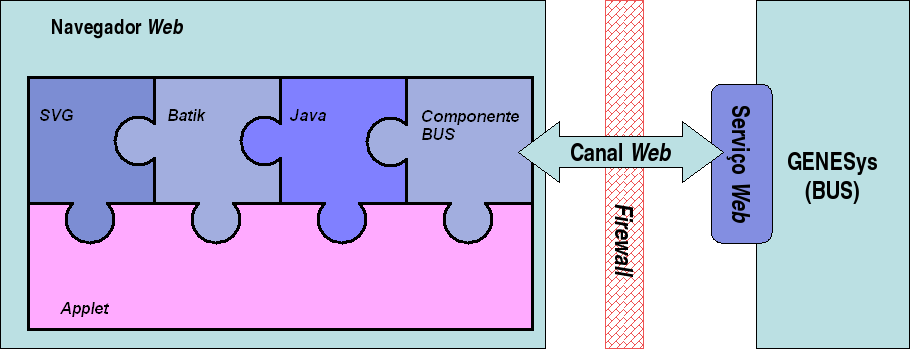
\includegraphics[width=0.86\textwidth]{puzzle}
    \caption{Architecture}
    \label{fig:arch}
\end{figure}

Loren ipsum dolor sit amet, consectetuer adipiscing elit. 
Praesent sit amet sem. Maecenas eleifend facilisis leo. Vestibulum et
mi. Aliquam posuere, ante non tristique consectetuer, dui elit
scelerisque augue, eu vehicula nibh nisi ac est. Nullam laoreet fermentum urna.

Duis eget diam. In est justo, tristique in, lacinia vel, feugiat eget,
quam. Pellentesque habitant morbi tristique senectus et netus et
malesuada fames ac turpis egestas. Fusce feugiat, elit ac placerat
fermentum, augue nisl ultricies eros, id fringilla enim sapien eu
felis. Vestibulum ante ipsum primis in faucibus orci luctus et
ultrices posuere cubilia Curae; Sed dolor mi, porttitor quis,
condimentum sed, luctus in. 

\subsection{Subsection Example} \label{sec:se322}

Suspendisse elementum sodales felis in Table~\ref{tab:example} is a 
floating table.

\begin{table}
  \caption{A table}
\begin{tabular}{|c|r@{.}lr@{.}lr@{.}l||r|}
	\hline
\multicolumn{8}{|c|}
	{\rule[-3mm]{0mm}{8mm}Iteration $k$ de $f(x_n)$} \\
\textbf{\em k}
	& \multicolumn{2}{c}{$x_1^k$}
	& \multicolumn{2}{c}{$x_2^k$}
	& \multicolumn{2}{c||}{$x_3^k$}
	& comments \\ \hline \hline
0   & -0&3                 & 0&6                 &  0&7   & - \\
1   &  0&47102965 & 0&04883157 & -0&53345964  & $\delta<\epsilon$ \\
2   &  0&49988691 & 0&00228830 & -0&52246185  & $\delta < \varepsilon$ \\
3   &  0&49999976 & 0&00005380 & -0&523656   &   $N$ \\
4   &  0&5                 & 0&00000307 & -0&52359743  & \\
\vdots	& \multicolumn{2}{c}{\vdots}
	& \multicolumn{2}{c}{$\ddots$}
	& \multicolumn{2}{c||}{\vdots}  & \\
7   &  0&5   & 0&0    & \textbf{-0}&\textbf{52359878}
		 & $\delta<10^{-8}$ \\ \hline
\end{tabular}
  \label{tab:example}
\end{table}

Loren ipsum dolor sit amet, consectetuer adipiscing elit. 
Praesent sit amet sem. Maecenas eleifend facilisis leo. Vestibulum et
mi. Aliquam posuere, ante non tristique consectetuer, dui elit
scelerisque augue, eu vehicula nibh nisi ac est. Suspendisse elementum
sodales felis. Nullam laoreet fermentum urna. 

Duis eget diam. In est justo, tristique in, lacinia vel, feugiat eget,
quam. Pellentesque habitant morbi tristique senectus et netus et
malesuada fames ac turpis egestas. Fusce feugiat, elit ac placerat
fermentum, augue nisl ultricies eros, id fringilla enim sapien eu
felis. Vestibulum ante ipsum primis in faucibus orci luctus et
ultrices posuere cubilia Curae; Sed dolor mi, porttitor quis,
condimentum sed, luctus in. 

\section{Section Example}

Loren ipsum dolor sit amet, consectetuer adipiscing elit. 
Praesent sit amet sem. Maecenas eleifend facilisis leo. Vestibulum et
mi. Aliquam posuere, ante non tristique consectetuer, dui elit
scelerisque augue, eu vehicula nibh nisi ac est. Suspendisse elementum
sodales felis. Nullam laoreet fermentum urna. 

\section{Summary}

Pellentesque habitant morbi tristique senectus et netus et
malesuada fames ac turpis egestas. Fusce feugiat, elit ac placerat
fermentum, augue nisl ultricies eros, id fringilla enim sapien eu
felis. Vestibulum ante ipsum primis in faucibus orci luctus et
ultrices posuere cubilia Curae; Sed dolor mi, porttitor quis,
condimentum sed, luctus in. 

%%%% Another chapter to force two pages in the index
%%%%
\chapter{Another chapter}

Integer nec quam. Sed fermentum. Nunc vitae leo. Etiam sit amet
quam. Nunc vestibulum massa in mauris. Duis eget nulla. 

\section{Section Example}

Fusce ultricies arcu eu nibh volutpat feugiat. Maecenas urna pede, 
commodo quis, porta eu, bibendum elementum, pede. 

\section{Section Example}

Sed eros massa, molestie eget, mattis non, rutrum ac, magna. 
Duis dui. Maecenas eget tortor ut dolor semper mattis. 
Maecenas auctor, tellus et ultricies tempor, elit
est placerat lacus, in posuere mauris lorem et arcu. 

\subsection{Subsection Example}

Nulla nec eros et pede vehicula aliquam. Aenean sodales pede vel
ante. Fusce sollicitudin sodales lacus. Maecenas justo mauris,
adipiscing vitae, ornare quis, convallis nec, eros. 

\subsection{Subsection Example}

Pellentesque pulvinar fringilla dolor. In sit amet pede. 
Proin orci justo, semper vel, vulputate quis, convallis
ac, nulla. Nulla at justo. Mauris feugiat dolor. 
Etiam posuere fermentum eros. Morbi nisl ipsum, tempus id, 
ornare quis, mattis id, dolor. Aenean molestie metus 
suscipit dolor. Aliquam id lectus sed
nisl lobortis rhoncus. Curabitur vitae diam sed sem aliquet
tempus. Sed scelerisque nisi nec sem.

\section{Section Example}

Sed eros massa, molestie eget, mattis non, rutrum ac, magna. 
Duis dui. Maecenas eget tortor ut dolor semper mattis. 
Maecenas auctor, tellus et ultricies tempor, elit
est placerat lacus, in posuere mauris lorem et arcu. 

\subsection{Subsection Example}

Nulla nec eros et pede vehicula aliquam. Aenean sodales pede vel
ante. Fusce sollicitudin sodales lacus. Maecenas justo mauris,
adipiscing vitae, ornare quis, convallis nec, eros. 

\subsection{Subsection Example}

Aliquam id lectus sed nisl lobortis rhoncus. 
Curabitur vitae diam sed sem aliquet tempus. Sed scelerisque 
nisi nec sem \textcite{khakipoor_linear_2023,liu_energy_2023}.

\section{Section Example}

Maecenas urna pede, commodo quis, porta eu, bibendum elementum, 
pede. Sed eros massa, molestie eget, mattis non, rutrum ac, 
magna. Duis dui. Maecenas eget tortor ut dolor semper mattis. 
Maecenas auctor, tellus et ultricies tempor, elit est placerat 
lacus, in posuere mauris lorem et arcu~\parencite{monopoli_exploiting_2023,zhang_carma_2023,chang_adas_2023, guo_rapidstream_2023}. 

\subsection{Subsection Example}

Nulla nec eros et pede vehicula aliquam. Aenean sodales pede vel
ante. Fusce sollicitudin sodales lacus. Maecenas justo mauris,
adipiscing vitae, ornare quis, convallis nec, eros. 

\subsection{Subsection Example}

Aliquam id lectus sed nisl lobortis rhoncus. 
Curabitur vitae diam sed sem aliquet tempus. Sed scelerisque 
nisi nec sem \textcite{khakipoor_linear_2023,liu_energy_2023} scelerisque.

Nulla nec eros et pede vehicula aliquam. Aenean sodales pede vel
ante. Fusce sollicitudin sodales lacus. Maecenas justo mauris,
adipiscing vitae, ornare quis, convallis nec, eros. Etiam laoreet
venenatis ipsum. In tellus odio, eleifend ac, ultrices vel, lobortis
sed, nibh. Fusce nunc augue, dictum non, pulvinar sed, consectetuer
eu, ipsum. Vivamus nec pede.  

%% Uncomment to see a listing example
%%%% an example on how to include code
%%% ---------------------------------
\section{Listing example}

Pellentesque habitant morbi tristique senectus et netus et
malesuada fames ac turpis egestas. Fusce feugiat, elit ac placerat
fermentum, augue nisl ultricies eros, id fringilla enim sapien eu
felis.

\begin{lstlisting}[language=Python, caption=Python example, label=code:useless]
# Take the user's input
words = input("Enter the text to translate to pig latin: ")
print(f"You entered: {words}")

# Break apart the words into a list
words = words.split(' ')

# Use a list comprehension to translate words greater than or equal to 3 characters
translated_words = [(w[1:] + w[0] + "ay") for w in words if len(w) >= 3 ]

# Print each translated word
for word in translated_words:
    print(word)
\end{lstlisting}

Listing~\ref{code:useless} uis eget diam. In est justo, tristique in, lacinia vel, feugiat eget,
quam. Pellentesque habitant morbi tristique senectus et netus et
malesuada fames ac turpis egestas. Fusce feugiat, elit ac placerat
fermentum, augue nisl ultricies eros, id fringilla enim sapien eu
felis. Vestibulum ante ipsum primis in faucibus orci luctus et
ultrices posuere cubilia Curae; Sed dolor mi, porttitor quis,
condimentum sed, luctus in.

\chapter{Introduction} \label{chap:intro}


\section{Context} \label{sec:context}

Lung cancer is the leading cause of cancer-related deaths and is often diagnosed at an advanced stage, contributing to a low 5-year survival rate of less than 10\%, which occurs in 70\% of cases. However, if detected early, the survival rate could exceed 90\%~\cite{ning_early_2021}. In 2022, lung cancer had the highest incidence and mortality rates of all cancers worldwide~\cite{international_agency_for_research_on_cancer_trachea_2024}. In particular, in upper-middle-income countries, there has been a significant increase in lung cancer-related deaths, with a rise of 442,000 deaths, more than 2.5 times the increase in deaths of the combined three other income groups~\cite{world_health_organization_top_2024}.

Efforts to reduce lung cancer mortality by screening have been hampered by the aggressive and diverse nature of the disease~\cite{national_lung_screening_trial_research_team_reduced_2011}. For example, low-dose \ac{ct} screening helps diagnose lung cancer more precisely and produces a reduction of 20\% in mortality. Today, the classification of a pulmonary nodule depends on measuring its growth rate from multiple \ac{ct} scans and following it for approximately two years to avoid performing a biopsy, which entails risks for patients and additional costs for healthcare entities. However, one significant drawback of conducting slice-by-slice \ac{ct} scans in lung cancer detection is that they are challenging for doctors since the process of obtaining this data is time-consuming, expensive, prone to reader bias, and requires a high degree of competence and concentration~\cite{shaffie_computer-assisted_2022}.

As medical data becomes more complex, there is a growing need for models that can effectively integrate and analyze this data to support clinical decision-making~\cite{iqbal_fusion_2023}. \ac{cad} is increasingly being investigated as an alternative and complementary approach to conventional reading, as it avoids many of these issues. Automated nodule diagnostic systems can save both time and money while avoiding the risks of invasive surgical procedures. The noninvasive \ac{cad} system for lung nodule diagnosis is promising and has achieved high accuracy from a single \ac{ct} scan~\cite{shaffie_computer-assisted_2022}.

The combined gains in medical imaging and \ac{dl} complement new approaches that are accurate and allow safer disease recognition. \ac{dl} models can overcome projections that show how medical images are analyzed to locate and determine the type of lung abnormalities that commonly cause cancer.


\section{Problem}\label{sec:problem}
This thesis addresses the need for a more accurate and reliable diagnostic tool. Existing diagnostic systems, primarily based on \ac{dl} models, have certain limitations regarding the accuracy and generalization of medical image datasets. These models are often based on deep features from neural networks, which can overshadow superficial features such as texture and shape that are important for accurately classifying nodules.

In addition, the lack of explainability of the model poses a challenge in clinical contexts, which can limit its reliability in making critical medical decisions. The inability to provide interpretable information hinders the adoption of these methods for diagnosing lung cancer.


\section{Hypothesis}\label{sec:hypothesis}
Feature extraction is critical for the characterization task. 
Although \acp{dnn}, are widely used to extract deep features, shallow features - such as texture and shape - can also be derived using traditional extractors. State-of-the-art works show that combining shallow and deep features can improve the effectiveness of \ac{dl} models in lung nodule characterization~\cite{xie_fusing_2018}.
These advancements highlight the need for further research in \ac{dl} and information fusion to prompt early detection, reduce mortality, and provide more effective treatment strategies for lung cancer patients.

We hypothesize that information fusion-based model approaches, with shallow and deep features, will result in a more accurate and reliable model for lung cancer characterization, making it better suited for early detection and precise diagnosis. We seek to overcome the current state-of-the-art limitations in automatic lung cancer diagnostics, offering a solution that not only improves prediction accuracy but also has the potential to assist in clinical decision-making and medical practice.


\section{Motivation}\label{sec:motivation}

Promoting the improvement of human life and health through the early detection of diseases continues to be a concern worldwide. Lung cancer is an enemy of public health care, and the development of early and accurate diagnostic tools will help improve survival rates.
This research aims to contribute to the goal of promoting health by harnessing modern technologies to address one of the most significant diagnostic issues in oncology today. By developing models that support more precise care, this dissertation aligns with the global imperative to promote well-being for all.


\section{Research Questions}\label{sec:questions}
We will break it down into three research questions to bring clarity and precision to the hypothesis. These questions will guide the investigation, helping us understand our hypothesis' main points.

\begin{enumerate}
    \item \textbf{Does fusing information from shallow and deep feature extractors improve classification or generalization performance when compared to using a deep approach only?}\\
    \item \textbf{How does the fusion approach behave under varying dataset conditions, such as different sample sizes, bounding‐box definitions, and image representations?}\\
    \item \textbf{In what ways does information fusion contribute to the explainability of lung nodule malignancy predictions?}\\
\end{enumerate}





 
%% \chapter{Literature Review} \label{chap:lreview}

The main goal of this literature review is to define a strategy for completing the state of research on information fusion-based models for lung nodule characterization, with a focus on identifying fusion techniques currently applied in this field. In particular, it has three main objectives: to gain knowledge by analyzing the different types of techniques that have been used in nodule characterization, to discover the specific methods that have been designed to automate nodule characterization and to evaluate the effectiveness of these methods based on the results obtained in the respective studies. However, in addition to achieving these objectives, the review will help to understand the current state of information fusion methods in this area and will lead to a better understanding of the various approaches.

Through recent studies analyses, we will study the most widely adopted techniques, as well as hybrid approaches that combine various strategies. In addition, methods used for automatic nodule characterization will also be analyzed, with a focus on deep learning architectures adapted to \ac{ct} scan image analysis. This synthesis aims to establish a comprehensive basis for future studies in the characterization of pulmonary nodules and to guide the development of more effective, interpretable and applicable models in a clinical environment.

\section{Eligibility Criteria} \label{criteria} 

In order to achieve the relevance and rigor of the selected studies, the criteria for the systematic review were specified. These criteria seek to encompass the entire body of research that has been conducted between shallow and deep feature extractors and information fusion techniques in the characterization of \ac{ct} scans, mainly related to lung nodules. To expand the scope, a more extensive view of applicable methodologies was included for medical conditions that use \ac{ct} technologies if the studies presented relevant approaches.

In terms of eligibility, only studies published in the last five years (2019 - 2024) were considered, which ensures that the review reflects recent advances in fusion techniques in the field of medical imaging. Articles were limited to those published in English to maintain consistency and accessibility. In addition to the characterization of pulmonary nodules, studies aimed at diagnosing other medical conditions revealed by \ac{ct} scans were also included, as long as they used methodologies that could be used within the scope of this study.

\section{Search Strategy}

In this review, a comprehensive search strategy was formulated to find relevant studies in various reliable databases. The search was conducted mainly in three academic databases: IEEE Xplore, PubMed and Google Scholar.

The search process employed a set of keywords and Boolean operators to develop comprehensive queries. The primary keywords included terms such as “lung nodule characterization,” “information fusion,” “shallow feature extraction,” “deep feature extraction,” and “\ac{ct} scan analysis.” Additionally, secondary terms were included to capture more specific methodologies and techniques, such as “texture features,” “shape features,” “convolutional neural networks (CNN),” and “medical image classification.”

Furthermore, in addition to the database searches, reference chaining was used to expand the list of studies. Specifically, the references of key articles excavated in the initial phase were subjected to scrutiny. As an example, significant references were extracted from the influential article Fusion of Textural and Visual Information for Medical Image Modality Retrieval Using Deep Learning-Based Feature Engineering~\cite{iqbal_fusion_2023}, which has been helpful in the study of fusion techniques for the analysis of pulmonary nodules. Reviewing the references cited in this document helped to identify other studies relevant to the objectives of the initial work, linked by common topics.



\section{Screening Process}

After the search drew out a set of studies that might be relevant, the title and abstract screening process followed. During this phase, each study's titles and abstracts were reviewed to weed out studies that are obviously not relevant. This first screening made it possible to discard the articles that didn't fit the core inclusion criteria, including those that are not associated with \ac{ct}-based medical imaging or those focusing on work unrelated to the use of shallow or deep features extractors or information fusion methods.

This strategy was used to cut out irrelevant studies in a fast and easy way as well as to let potentially related papers through to the full-text analysis phase. At this stage, the objective was to screen only titles and abstracts. This enabled the easy inclusion of studies that were worth further investigation in subsequent stages.

\newpage
\section{Summary}

This literature review lays the foundations for the study and research into lung nodule characterization models based on information fusion. With the implementation of a search strategy, this review presents a current selection of studies focused on the characterization of lung nodules and including other diseases based on \ac{ct} scans. The structured procedure of using the main databases and linking references ensures that relevant studies are obtained, and the selection is further boosted by the use of the title and abstract screening process, which shortens the selection to studies that are actually dealing with research in terms of deep learning, shallow feature extraction and information fusion techniques.
 %% Needed only for PDIS
%% \chapter{Methodology planning }\label{chap:chap4}
In summary, this workplan outlines a systematic and rigorous approach to developing a robust pulmonary nodule classification system. By integrating advanced deep learning models with complementary shallow feature extractors and employing sophisticated fusion methods, the study aims to achieve significant improvements in diagnostic accuracy and robustness, with clear pathways for addressing potential limitations and risks.
%% Detailed Work Plan / Activity cards
    %% Task Identification
    %% Duration, begin and end dates
    %% Goals and expected outcomes
    %% Detailed description (may include materials and methods)
    %% Deliverables
    %% Milestones
%% Description
%% Experimental process & Evaluation Design
    %% Introduction
    %% Research design
    %% Research context
    %% Population and sampling
    % LIDC-IDRI as example
%% Expected Results

%% Conclusion
    %% Ethical considerations
    
    %% Problem and goals
    %% Limitations Acknowledge
    
    %% Conclusions drawn from the related work and gap analysis
    
    %% SMART analysis of the project goals
    %% SWOT analysis of the project proposal
    
    
    %% Mitigation plan
    %% Risk assessment and contingency plan
\section{Population and sampling}
    The lung nodule classification study will use a population of \ac{ct} images from publicly available and clinically validated datasets, generally used for this purpose. We will fully trust in their assignment of labels (benign/malignant) to conduct experiments. 
    
    To retrieve insights into the characteristics and quality of the data we will submit it to an analysis and provide some visualization for easier interpretation. Computing and summarizing statistics such as mean, median, and standard deviation, for nodule size, patient demographics, and other clinical variables and distribution of classifications in the used datasets to evaluate balance and ascertain the need to perform sampling techniques. For each dataset selected, pre-processing will be carried out in order to improve the quality of the images: ensuring uniformity if necessary, such as applying resampling techniques, and removing, for example, noise and other irrelevant information.
    
    In order to proceed with the experimentation phase, the data will be randomly divided into training and test sets, with the aim of carrying out evaluations afterward. This division will mitigate possible over-fitting effects.
        
\section{Evaluation Strategy}
Each combination will be evaluated using standardized cross-validation protocols to ensure robust and generalizable results. Detailed logs of the performance metrics for each run will be maintained to enable comprehensive comparative analysis.
Accuracy provides an overall measure of the model’s correctness by quantifying the proportion of correctly classified cases. However, accuracy alone can be misleading in imbalanced datasets, where the majority class dominates predictions. Sensitivity (recall) is essential in this context, as it measures the model's ability to correctly identify malignant nodules, ensuring minimal false negatives, which is critical for early cancer detection and patient prognosis. Conversely, specificity assesses the model’s capability to correctly classify benign nodules, reducing false positives and preventing unnecessary invasive procedures. Finally, the area under the receiver operating characteristic curve (AUC-ROC) provides a comprehensive assessment of the model's discriminative ability across various decision thresholds, balancing sensitivity and specificity.

\section{Deep-Learning Selection}
The first step in the research is to detect and manifest deep learning models that are the best of the best and specifically designed for the classification of pulmonary nodules in \ac{ct} images. The primary target is to create a baseline for performance measurements that are to be taken into consideration. The retrieve models will be subject of a defined evaluation and ranked based on performance. We will use the best performing models to combine them with additional methods and features. 

\section{Shallow Extractors}
In parallel with deep learning, shallow feature extractors are employed to capture complementary visual and textural information about pulmonary nodules. This stage aims to identify and implement diverse extractors that contribute unique feature sets. We will select the most used extractors for texture, shape, moment-based, gradient-based, and hierarchical features used in the state of the art.
The objective is to use them in the same dataset used for deep learning methods and ensuring compatibility with fusion techniques.

\section{Fusion Methods}
The integration of deep learning outputs with shallow feature sets is crucial for leveraging the strengths of both approaches. To achieve this, state-of-the-art fusion techniques will be examined and implemented. Fusion can be applied at two primary levels: decision-level and feature-level. Decision-level fusion combines predictions from multiple models or classifiers using techniques such as weighted voting, majority voting (MAX-VOTE), and prediction averaging, allowing the ensemble of predictions to refine the overall accuracy. On the other hand, feature-level fusion involves concatenating or averaging feature vectors from deep learning models and shallow extractors, often with dimensionality reduction techniques like \ac{PCA} to manage high-dimensional data. These techniques will be implemented in a modular framework, ensuring compatibility with various model configurations.

\section{Experimentation}
The experimentation phase is designed to systematically evaluate the performance of different combinations of deep learning models, shallow feature extractors, and fusion techniques in classifying pulmonary nodules. A flexible workflow will be developed to facilitate the testing of these combinations. This workflow begins by selecting one of the three top-performing deep learning models identified earlier, followed by choosing one to all five shallow feature extractors. The selected outputs are then combined using one of the chosen fusion methods. The pipeline processes the input \ac{ct} images, extracts features, applies fusion, and trains the combined model. For each configuration, the model's performance will be assessed using metrics such as accuracy, sensitivity, specificity, F1-score, area under the curve (AUC), and false-positive rate (FPR).
This systematic approach ensures that all potential interactions between deep learning models, shallow feature extractors, and fusion techniques are explored. The goal is to identify the configurations that deliver the highest classification accuracy, outperforming both standalone deep learning models and traditional classifiers. The experimental results will provide valuable insights into the synergies between deep and shallow methods, establishing a robust foundation for future advancements in pulmonary nodule classification.

\section{Expected Results}

We anticipate that the proposed model will demonstrate significant improvements over baseline methods. Specifically, the study expects: to improve the accuracy, sensitivity, specificity, and AUC-ROC of defined baselines and other state of the art approaches; to achieve a robust performance on unseen datasets, indicating effective generalization; to prove the combined use of deep learning and shallow features will result in a model with an higher discriminative ability; to enhance interpretability and manage computational demands through design and potential use of specialist models.


\section{Conclusion}

The research will exclusively use publicly available datasets, ensuring compliance with ethical standards and privacy guidelines. Since no new patient data will be collected and because no sensitive data is located in the datasets, the ethical risks are negligible.

We knowledge that the research could be held back due to parameter configurations difficulties, challenges on accurately segmenting complex nodule cases and the possibility that the selected data sets might not fully represent the diversity found in the clinical contexts required for implementation in diagnostics.


To address potential challenges, techniques will be applied to mitigate overfitting and in case of training or data challenges, the approach includes the flexibility to simplify the model or adopt alternative (or simpler) methods.
Other risks, such as delays, dataset issues, or training difficulties will be monitored, in order to mitigate them and resolve problems before they cause major delays and other conflicts that are more difficult to predict and control.

\subsection{SWOT Analysis}
\begin{tcbraster}[raster columns=2, boxrule=0mm, arc=0mm]
\begin{tcolorbox}[equal height group=A, size=fbox, colback=swotS!60, colframe=swotS!80!black, title=\textsc{strengths}]
\begin{enumerate}
    \item Use of deep and shallow extractors fused with advanced strategies.
    \item Access to clinically validated, publicly available datasets.
    \item Rigorous evaluation protocols.
\end{enumerate}
\end{tcolorbox}
\begin{tcolorbox}[equal height group=A, size=fbox, colback=swotW!60, colframe=swotW!80!black, title=\textsc{weaknesses}]
\begin{enumerate}
    \item Highly dependent on training set demographics representation.
    \item High computational resource requirements.
    \item Complexity in integrating multiple methodologies.
\end{enumerate}
\end{tcolorbox}
\begin{tcolorbox}[equal height group=B, size=fbox, colback=swotO!60, colframe=swotO!80!black, title=\textsc{opportunities}]
\begin{enumerate}
    \item Development of novel fusion strategies and architectures.
    \item Contribution to advancements in CAD systems.
\end{enumerate}
\end{tcolorbox}
\begin{tcolorbox}[equal height group=B, size=fbox, colback=swotT!60, colframe=swotT!80!black, title=\textsc{threats}]
\begin{enumerate}
    \item New competing methods and research in the field.
    \item Variability in image data that could impact model performance.
    \item Compliance with clinical and regulatory requirements.
\end{enumerate}
\end{tcolorbox}
\end{tcbraster}

\subsection{Work Plan}
\begin{ganttchart}[
    hgrid,
    vgrid,
    title height=1,
    bar height=0.6
]{0}{20}
    \gantttitle{Work Plan by Week}{21} \\
    \gantttitlelist{0,...,20}{1}{} \\

    % SOTA and Data Collection Phase
    \ganttbar{SOTA Revision and Improvement}{0}{1} \\
    \ganttmilestone{SOTA Finalized}{1} \\
    \ganttbar{Data Selection and Sampling}{1}{2} \\
    \ganttbar{Data Analysis and Visualization}{2}{3} \\
    
    % Data Pre-Processing Phase
    \ganttbar{Data Pre-Processing}{3}{4} \\
    \ganttmilestone{Prepared Data}{4} \\

    % Evaluation and Model Development
    \ganttbar{Evaluation Workflow Development}{4}{6} \\
    \ganttbar{Deep Learning Selection}{5}{6} \\
    \ganttbar{Shallow Feature Extraction}{6}{7} \\
    \ganttbar{Fusion Methods Selection}{7}{8} \\
    \ganttmilestone{Experiment Subjects Finalized}{8} \\

    % Experimentation and Tuning
    \ganttbar{Experimentation Phase}{8}{16} \\
    \ganttbar{Model Tuning}{10}{16} \\
    \ganttmilestone{Experimentation Completed}{16} \\

    % Thesis Writing and Final Adjustments
    \ganttbar{Thesis Writing Draft}{7}{16} \\
    \ganttmilestone{Thesis Draft Finalized}{16} \\
    \ganttbar{Contingencies and Final Adjustments}{16}{20} \\
    \ganttmilestone{Final Adjustments Completed}{20} \\
    
\end{ganttchart}



 %% Needed only for PDIS
\chapter{Theoretical Background}\label{chap:background}

\section{Medical and Clinical Context}\label{sec:med_context}

\subsection{Lung Cancer}

Most of the lung cancer cases diagnosed at a symptomatic stage are related to the primary or metastatic disease or some paraneoplastic syndrome. The process of patient evaluation involves physical examination, \ac{ct} scans of the thorax and abdomen, pulmonary function tests, laboratory tests, monitoring patient weight loss and retrieving tumor tissue to perform histologic diagnosis, in order to determine the stage of the disease based on the international \ac{tnm} staging system~\cite{minna_focus_2002, watanabe_tnm_2003}.

Four major histologic lung cancer types comprise the majority of them, including small cell lung cancer and three non-small cell lung cancer types~\cite{travis_pathology_2011}.
Small cell lung cancer and squamous cell carcinoma arise mainly in the central airways, while adenocarcinomas are located more peripherally. The large-cell carcinoma is less differentiated from the other non-small cell lung cancer types and arises from metaplastic changes resulting from smoking.

Patients with small-cell lung cancer confined to the chest undergo treatment that includes thoracic radio and chemotherapy. In contrast, patients with more advanced stages of the disease receive chemotherapy along with various other drug combinations. Treatments normally result in tumor shrinkage, symptom relief, and an increase in median survival~\cite{minna_focus_2002}.

On the other hand, patients with non-small cell lung cancer whose disease is confined to the chest undergo surgical evaluation of the mediastinum to check for lymph node involvement. More recently, they have also been subjected to \ac{pet} scans, a functional imaging technique that detects radiotracer uptake to assess metabolic activity, providing complementary information ~\cite{buzug_computed_2011}.
In the cases where there is no evidence of mediastinal lymph node involvement or distant metastatic disease, patients have surgical resection of the primary tumor. Those with mediastinal lymph node involvement are submitted either to (1) preoperative chemotherapy followed by an attempt at surgical resection, as in the previous case, or (2) a combination of chemotherapy and chest radiotherapy administered as part of a curative treatment strategy. These therapies may not cure the condition, but they can relieve symptoms and extend life by 2 to 10 months~\cite{minna_focus_2002}.


\subsection{Lung Nodule}
According to \textcite{baum_incidental_2024, loverdos_lung_2019}, a lung nodule can be defined "as a more or less round, well-demarcated lesion measuring up to 3 cm in diameter".

Lung nodules in \ac{ct} imaging are classified into three distinct categories based on their attenuation: solid nodules, the most common form, characterized by a consistent homogeneous soft-tissue attenuation; ground-glass nodules, which present a non-uniform appearance with a hazy increase in local attenuation of the lung parenchyma, while still clearly displaying the underlying bronchial and vascular structures; and part-solid nodules, which include both solid and ground-glass attenuation components~\cite{loverdos_lung_2019}.

Incidental detection of pulmonary nodules is prevalent, occurring in up to 75\% of \ac{ct} scans performed for other clinical reasons, with more than half of patients presenting with two or more nodules. In this context, morphological assessment by \ac{ct} plays a crucial role in stratifying the risk of malignancy. Specific benign lesions show characteristic morphological patterns that allow for non-invasive diagnosis. For example, granulomas often show central, laminar, or diffuse calcifications, while the presence of "popcorn" calcifications is pathognomonic of hamartomas. In addition, well-defined perifissural nodules are generally benign lymph nodes with an extremely low risk of malignancy~\cite{baum_incidental_2024}.

The increasing occurrence of incidental findings in asymptomatic individuals undergoing imaging poses notable challenges in clinical practice. One major issue is the overestimation of minor nodule volumes due to the partial volume effect, which can result in inaccurate assessments and potential misclassification~\cite{larici_lung_2017}. Additionally, distinguishing between benign and malignant nodules is complex, potentially resulting in delayed diagnoses or unnecessary invasive procedures.
This diagnostic uncertainty is worsened by the absence of standardized and reliable management algorithms, which are essential for the timely detection and treatment of malignant lesions~\cite{loverdos_lung_2019}.

By effectively addressing these challenges and accurately interpreting imaging characteristics to assess the risk of malignancy, healthcare providers can improve the precision of screening practices. This strategy significantly decreases the need for unnecessary invasive diagnostic procedures, ultimately leading to safer, more efficient, and cost-effective clinical follow-up for patients.

\section{Medical Imaging and CT Scans}\label{sec:med_image}

\subsection{Computed Tomography}\label{subsec:ct}

\acf{ct} is an imaging modality that uses X-ray technology to generate detailed cross-sectional images of the body by measuring the attenuation of X-ray beams as they pass through different tissues.
The attenuation caused by the absorption and scattering of some photons prevents them from reaching the detector, resulting in a record of this variation at different angles during a complete rotation.
The projections are then reconstructed in a 3D volume made up of volumetric pixels (voxels). Each pixel is assigned a \ac{ct} number, measured in \ac{hu}, which reflects the local attenuation of the X-rays corresponding to the density of the tissue (air has -1000 \ac{hu}, water has 0 \ac{hu}, and values above 400 \ac{hu} indicate the density of hard tissues)~\cite{rodrigues_efficient-proto-caps_2025}. In spatial resolution, each voxel shares the respective dimension with the pixels present in the X and Y axes of the image, while the slice thickness determines the Z dimension~\cite{cantatore_introduction_2011, buzug_computed_2011, mazonakis_computed_2016}.

The process of generating a \ac{ct} scan involves several key steps: scanning of an object with a specific configuration and parameters (such as magnification, orientation, X-ray energy); reconstruction of 2D projections in a 3D vortex matrix; determining a threshold value for accurate segmentation; generating surface or volume data; and conducting dimensional measurements or geometric analysis~\cite{cantatore_introduction_2011}.

\subsection{Screening Challenges}

When tasked with evaluating the malignancy of lung nodules, the first step is to segment the lung parenchyma\footnote{The functional tissue of an organ as distinguished from the connective and supporting tissue.
}, followed by the segmentation of the nodules. Large solid nodules ($> 10 mm$) present a unique challenge for identification, as they have a different intensity range compared to smaller lesions.
Predicting lung cancer at an early stage using \ac{ct} images poses significant challenges for radiologists. This process requires a significant investment of time and resources, and it is susceptible to errors. Screening requires a high level of concentration and expertise due to various factors, including low contrast variation, heterogeneity, and the visual similarities between benign and malignant nodules~\cite{jassim_systematic_2022}.

Accurate detection of lung nodules is a difficult task in the field of medical imaging. The nodules are often extremely unbalanced, exhibiting high intra-class variance, and the complex structure of the lungs further complicates this issue.


\section{Handcrafted Features in Radiomics}\label{sec_features}

Radiomics is a topic of much discussion in the fields of nuclear medicine and medical imaging. It aims to extract quantitative and reproducible insights from diagnostic images by capturing complex patterns that are often difficult for the human eye to recognize or measure~\cite{cantatore_introduction_2011}.

These features can be classified into the following categories: statistical, which includes histogram-based and texture-based; model-based; transform-based; and shape-based, derived from the type of information that is extracted and the way it is extracted
~\cite{cantatore_introduction_2011, abbasian_ardakani_interpretation_2022}.
To enhance readability, we use the term \ac{roi} to refer to both 2D areas and 3D volumes.

In the following sections, we will provide an overview of the features used in this thesis, as well as others that help to understand them.

\subsection{First-Order Features}

\acf{fof}, often known as histogram-based features or intensity features, describe the distribution of voxel intensities within a region of interest and are derived from the histogram of an image. These features are computed using the gray-level histogram and provide the simplest information extracted from the image. They specifically reflect individual voxel intensities without taking into account any relationships with neighboring voxels~\cite{abbasian_ardakani_interpretation_2022}.

We will assume the following foundational premises~\cite{van_griethuysen_computational_2017}:
\begin{itemize}
  \item $\mathbf{X}$ is the set of $N_p$ voxels included in the \ac{roi}.
  \item $\mathbf{P}(i)$ is the first-order histogram with $N_g$ discrete intensity levels, where $N_g$ is the number of non-zero bins, equally spaced from 0 with a width defined by the \texttt{binWidth} parameter.
  \item $p(i)$ is the normalized first-order histogram, defined as $p(i) = \frac{\mathbf{P}(i)}{N_p}$.
\end{itemize}

\subsubsection*{Energy}
Energy serves as a quantitative measure of the magnitude of voxel values within an image. Higher voxel values indicate a greater cumulative total of the squares of these values, reflecting enhanced intensity characteristics within the image data.

\begin{equation}
    \textit{energy} = \displaystyle\sum^{N_p}_{i=1}{(\textbf{X}(i))^2}
\end{equation}

\subsubsection*{Total Energy}
Total Energy represents the quantitative measure of the Energy feature, adjusted by the volume of the voxel, expressed in cubic millimeters.

\begin{equation}
    \textit{total energy} = V_{voxel}\displaystyle\sum^{N_p}_{i=1}{(\textbf{X}(i))^2}
\end{equation}

\subsubsection*{Entropy}
Entropy is a quantitative measure of the uncertainty and randomness inherent in image voxel values, capturing the average information content required for the encoding of those values.

\begin{equation}
    \textit{entropy} = -\displaystyle\sum^{N_g}_{i=1}{p(i)\log_2\big(p(i)\big)}
\end{equation}

\subsubsection*{Minimum}
This feature refers to the smallest gray level intensity value within the \ac{roi}, representing the lowest voxel value detected in the analyzed area.  
\begin{equation}
    \textit{minimum} = \min(\textbf{X})
\end{equation}

\subsubsection*{10$^{\text{th}}$ percentile}
This value indicates that 10\% of the gray level intensities within the \ac{roi} fall below this threshold.
This metric offers insight into the lower end of the intensity distribution, assisting in characterizing the presence of darker regions. 

\subsubsection*{90$^{\text{th}}$ percentile}
This value signifies that 90\% of the gray level intensities in the \ac{roi} are below this mark.
The 90$^{\text{th}}$ percentile underscores the upper range of intensity distribution, highlighting the presence of brighter regions.  

\subsubsection*{Maximum}
 This denotes the largest gray level intensity value found within the \ac{roi}, reflecting the highest voxel value identified in the analyzed area and representing the brightest point within that region.  
\begin{equation}
    \textit{maximum} = \max(\textbf{X})
\end{equation}

\subsubsection*{Mean}
The mean refers to the average gray level intensity calculated from all voxel values within the given \ac{roi}.
\begin{equation}
    \textit{mean} = \frac{1}{N_p}\displaystyle\sum^{N_p}_{i=1}{\textbf{X}(i)}
\end{equation}

\subsubsection*{Median}
The median refers to the middle value of gray-level intensities within the \ac{roi} when the values from the voxels are ordered. 

\subsubsection*{Interquartile Range}
The \acf{iqr} is defined as the difference between the 75th percentile ($\mathbf{P}_{75}$) and the 25th percentile  ($\mathbf{P}_{25}$) of a data set. 

\begin{equation}
    \textit{IQR} = \textbf{P}_{75} - \textbf{P}_{25}
\end{equation}



\subsubsection*{Range}
The range of a dataset is calculated as the difference between the maximum and minimum values of the observed data.
\begin{equation}
    \textit{range} = \max(\textbf{X}) - \min(\textbf{X})
\end{equation}

\subsubsection*{Mean Absolute Deviation}
The \acf{mad} quantifies the average distance of all intensity values from the overall mean value of the image array. This statistic provides insights into the degree of variation present within the intensity levels.
\begin{equation}
    \textit{MAD} = \frac{1}{N_p}\displaystyle\sum^{N_p}_{i=1}{|\textbf{X}(i)-\bar{X}|}
\end{equation}

\subsubsection*{Robust Mean Absolute Deviation}
The \acf{rmad} measures the average distance of intensity values from the mean calculated from a subset of the image array. This subset consists of gray levels that fall within the range of the 10th to the 90th percentiles.
\begin{equation}
\textit{rMAD} = \frac{1}{N_{10-90}}\displaystyle\sum^{N_{10-90}}_{i=1}
      {|\textbf{X}_{10-90}(i)-\bar{X}_{10-90}|}
\end{equation}

\subsubsection*{Root Mean Squared}
\acf{rms} is defined as the square root of the mean of the squared intensity values. This metric serves as an alternative measure of the overall magnitude of the image values.
\begin{equation}
    \textit{RMS} = \sqrt{\frac{1}{N_p}\sum^{N_p}_{i=1}{(\textbf{X}(i))^2}}
\end{equation}

%\subsubsection*{Standard Deviation}
%\begin{equation}
%\textit{standard deviation} = \sqrt{\frac{1}{N_p}\sum^{N_p}_{i=1}{(\textbf{X}(i)-\bar{X})^2}}
%\end{equation}
%
\subsubsection*{Skewness}
Skewness quantifies the asymmetry of a distribution in relation to its mean. It indicates whether the distribution's tail extends more towards the higher or lower values, which results in positive or negative skewness depending on the concentration of the data.
\begin{equation}
    \textit{skewness} = \displaystyle\frac{\mu_3}{\sigma^3} =
        \frac{\frac{1}{N_p}\sum^{N_p}_{i=1}{(\textbf{X}(i)-\bar{X})^3}}
        {\left(\sqrt{\frac{1}{N_p}\sum^{N_p}_{i=1}{(\textbf{X}(i)-\bar{X})^2}}\right)^3}
\end{equation}
Having $\mu_3$ as the 3$^{\text{rd}}$ central moment.

\subsubsection*{Kurtosis}
Kurtosis is a statistical measure that describes the 'peakedness' of the distribution of values within the image \ac{roi}. A higher kurtosis indicates that the distribution's mass is concentrated towards the tails rather than the mean. Conversely, a lower kurtosis suggests that the mass is more focused around a spike near the mean value.
\begin{equation}
    \textit{kurtosis} = \displaystyle\frac{\mu_4}{\sigma^4} =
        \frac{\frac{1}{N_p}\sum^{N_p}_{i=1}{(\textbf{X}(i)-\bar{X})^4}}
        {\left(\frac{1}{N_p}\sum^{N_p}_{i=1}{(\textbf{X}(i)-\bar{X}})^2\right)^2}
\end{equation}
Having $\mu_4$ as the 4$^{\text{th}}$ central moment.
\subsubsection*{Variance}
Variance is defined as the mean of the squared distances of each intensity value from the overall mean value. By definition, variance is represented as $\sigma^2$.
\begin{equation}
    \textit{variance} = \frac{1}{N_p}\displaystyle\sum^{N_p}_{i=1}{(\textbf{X}(i)-\bar{X})^2}
\end{equation}

\subsubsection*{Uniformity}
Uniformity quantifies the sum of the squares of intensity values, serving as an indicator of an image array's homogeneity. Higher uniformity signifies greater homogeneity and a reduced range of discrete intensity values.
\begin{equation}
    \textit{uniformity} = \displaystyle\sum^{N_g}_{i=1}{p(i)^2}
\end{equation}


\subsection{Texture-based Features}
In the words of \textcite{kaur_review_2021}, "A textural feature is nothing more than a recurrent arrangement of information in a visual representation". 

Textures provide valuable information about an object's material properties, spatial organization, and surrounding environment.
Since the textural properties of images contain helpful information for distinguishing between different objects, it is essential to incorporate texture features into the analysis~\cite{haralick_textural_1973}.

By extracting these texture features, we can improve the ability of algorithms to differentiate between various classes of images and identify specific patterns within them. 

\subsubsection{Gray-Level Co-Occurrence Matrix}
The \acf{glcm} is a statistical method used to analyze textures by considering the spatial relationships between pixels. This technique characterizes an image's texture by quantifying how frequently pairs of pixels with specific values occur in a defined spatial arrangement~\cite{zulpe_glcm_2012}.

In the generation of a \ac{glcm}, each element located at position (i, j) represents the aggregated count of occurrences where a pixel with the intensity value i is found in a specific spatial relationship to a pixel with the intensity value j within the given input image. This matrix captures the frequency of pixel value pairs at a defined distance and orientation, thereby providing insights into the spatial distribution of pixel intensities. Essentially, for each pair of pixel values (i, j), the \ac{glcm} tallies how many times pixels of value i are adjacent to pixels of value j according to the chosen configuration, such as horizontal, vertical, or diagonal arrangements~\cite{zulpe_glcm_2012}.

\subsubsection{Haralick Features}
Based on the \ac{glcm}, also referred to in earlier literature as the \acf{gtsdm}, \textcite{haralick_textural_1973} proposed a comprehensive suite of 28 textural features that could be extracted from each image matrix. They collected four values for each of the 14 measures and then calculated the average and range for each measure based on these four values~\cite{haralick_textural_1973, zulpe_glcm_2012}. This resulted in a total of 28 features that could be used as inputs for a classifier. 

Let us first establish the needed notation for the calculation of the 14 features:

\begin{itemize}

  \item $p(i,j)$: Normalized value of the \ac{glcm} at row $i$ and column $j$.
  
  \item $p_x(i)$: $i$$^{\text{th}}$ entry in the marginal-probability matrix obtained by summing the rows of $p(i,j)$,\\
  $p_x(i) = \sum_{j=1}^{N_g} p(i,j)$.
  
  \item $N_g$: Number of distinct gray levels  in the quantized
 image (size of the \ac{glcm})
  
  \item $\sum_i$ and $\sum_j$, shorthand for $\sum_{i=1}^{N_g}$ and $\sum_{j=1}^{N_g}$, respectively.
  
  \item $p_y(j) = \sum_{i=1}^{N_g} p(i,j)$
  
  \item $p_{x+y}(k) = \sum_{\substack{i=1 \\ j=1 \\ i+j=k}}^{N_g} p(i,j), \quad k = 2,3,\ldots,2N_g$
  
  \item $p_{x-y}(k) = \sum_{\substack{i=1 \\ j=1 \\ |i-j| = k}}^{N_g} p(i,j), \quad k = 0,1,\ldots,N_g - 1$
\end{itemize}

The presented equations define the proposed features:
\begin{enumerate}
\newcommand{\tightitem}[1]{\begin{samepage}\item #1\end{samepage}}
    \item \textbf{Angular Second Moment:}\\
    \acf{asm} quantifies the homogeneity of an image and is defined as~\cite {haralick_textural_1973}:
        \begin{equation}
            \text{ASM} = \sum_{i} \sum_{j} p(i,j)^2
        \end{equation}
    When the pixels present in a given image are very similar, the \ac{asm} value will be significant. In a quantization scheme with $(N_g)$ gray levels, a uniform image will have only one entry in the \ac{glcm}, resulting in a maximum \ac{asm} value of 1. In contrast, given an image that is filled completely randomly, all entries of the $(N_g \times N_g)$ \ac{glcm} matrix will be equally represented, with the probability of each entry defined by $p(i, j) = {1}/{N_g^2}$.
    This results in the minimum \ac{asm} value being ${1}/{N_g^2}$~\cite{oprisan_bounds_2023}.

    High energy values are indicative of a constant or periodic gray-level distribution. Energy is defined within a normalized range, and the \ac{glcm} of an image with lower homogeneity will display numerous small entries~\cite{oprisan_bounds_2023}.
    
    \item \textbf{Contrast:}\\
    Contrast measures the local variations present in the image and is defined as follows~\cite {haralick_textural_1973}:
        \begin{equation}
            \text{Contrast} = \sum_{n=0}^{N_g - 1} n^2 \left[ \sum_{i=1}^{N_g} \sum_{j=1}^{N_g} p(i,j) \quad \text{where} \quad |i - j| = n \right]
        \end{equation}
        
    \item \textbf{Correlation:}\\
    Correlation explains the relationship between a reference pixel and its neighbor: 0 signifies no correlation, while 1 indicates perfect correlation. This measure is analogous to the known Pearson correlation coefficient~\cite{oprisan_bounds_2023}.
        \begin{equation}
            \text{Correlation} = \frac{\sum_{i} \sum_{j} (i - \mu_i)(j - \mu_j) p(i,j)}{\sigma_i \sigma_j}
        \end{equation}
    $\mu_i$: Mean of row marginals: $\mu_i = \sum_{i=1}^{N} i \cdot \sum_{j=1}^{N} p(i,j)$ \\
    $\mu_j$: Mean of column marginals: $\mu_j = \sum_{j=1}^{N} j \cdot \sum_{i=1}^{N} p(i,j)$ \\
    $\sigma_i$: Standard deviation of row marginals. \\
    $\sigma_j$: Standard deviation of column marginals.\\
        
    \item \textbf{Variance:}\\
    Variance, also known as the Sum of Squares, measures how the values are dispersed around the mean of reference and neighboring pixels. 
    Its value increases when the gray-level values deviate from their mean~\cite{oprisan_bounds_2023}.
        \begin{equation}
            \text{Variance} = \sum_{i} \sum_{j} (i - \mu)^2 p(i,j)
        \end{equation}
      $\mu$: Mean intensity of the \ac{glcm}: $\mu = \frac{1}{N_g}\sum_{i=1}^{N_g} \sum_{j=1}^{N_g} p(i,j)$ \\
    
    \item \textbf{Inverse Difference Moment:}\\
    \acf{idm} measures the homogeneity of an image by giving larger values to smaller gray-tone differences between pairs of elements. This metric is particularly sensitive to near-diagonal elements in the \ac{glcm}. \ac{idm} reaches its maximum value when all elements in the image are identical~\cite{oprisan_bounds_2023}.
    Its definition is as follows:
        \begin{equation}
            \text{IDM} = \sum_{i=1} \sum_{j=1} \frac{p(i,j)}{1 + (i - j)^2}
        \end{equation}
        
    \item \textbf{Sum Average:}\\
    Represent the sum of the average of all gray levels.
        \begin{equation}
            \text{Sum Average} = \sum_{i=2}^{2N_g} i \cdot p_{x+y}(i)
        \end{equation}
        
    \item \textbf{Sum Variance:}\\
    It represents a heterogeneity measure that assigns higher weights to intensity level pairs from neighbors that deviate more from the mean~\cite{oprisan_bounds_2023}.
        \begin{equation}
            \text{Sum Variance} = \sum_{i=2}^{2N} (i - \text{Sum Average})^2 p_{x+y}(i)
        \end{equation}  
        
    \item \textbf{Sum Entropy:}\\
    Sum entropy measures the non-uniformity present in an image, and in this case, the complexity of the texture~\cite{oprisan_bounds_2023}.
    
        \begin{equation}
            \text{Sum Entropy} = -\sum_{i=2}^{2N} p_{x+y}(i) \log p_{x+y}(i)
        \end{equation}
        Since some of the probabilities may be zero, and $log(0)$ is not defined, \textcite{haralick_textural_1973} recommended that the term $log (p + \epsilon)$ be used in place of $log (p)$ in entropy computations, having $\epsilon$ as an arbitrarily small positive constant.
        
    \item \textbf{Entropy:}\\
    Entropy measures the complexity or randomness within an image by analyzing the distribution of values in the \ac{glcm}. It reaches its maximum when all entries in the \ac{glcm} are equally probable, indicating a state of maximum disorder. Also known as "Shannon entropy," this metric is high when the matrix contains a wide variety of small, non-uniform values, which reflects complex and heterogeneous textures~\cite{oprisan_bounds_2023}.
        \begin{equation}
            \text{Entropy} = -\sum_{i} \sum_{j} p(i,j) \log p(i,j)
        \end{equation}
    Since entropy is inversely related to \ac{asm} (or Energy), images with intricate, non-repetitive patterns tend to exhibit high entropy and low Energy.
        
    \item \textbf{Difference Variance:}\\
    Represents the variance of the difference between gray levels.
        \begin{equation}
            \text{Difference Variance} = \sum_{k}^{2N_g} (k - \text{DA})^{2} p_{x-y}(k)
        \end{equation}

    Where Difference Average: \quad {DA} = $\sum_k^{2N_g} k p_{x-y}(k)$ 
        
    \item \textbf{Difference Entropy:}\\
    Difference entropy is a quantitative measure used to assess the level of randomness or disorder present in the contrast of an image~\cite{oprisan_bounds_2023}.
        \begin{equation}
            \text{Difference Entropy} = -\sum_{i=0}^{N_g-1} p_{x-y}(i) \log p_{x-y}(i)
        \end{equation}
        
    \item 13. \textbf{Information Measures of Correlation}\\
    \acf{imc} involves analyzing different parameters using various techniques. Mutual information is normalized, and information correlation is set to infinity when the denominator is zero~\cite{oprisan_bounds_2023}.
        \begin{equation}
            \text{IMC1} = \frac{HXY - HXY1}{\max(HX, HY)}
        \end{equation}
        \begin{equation}
            \text{IMC2} = \sqrt{1 - \exp[-2(HXY2 - HXY)]}
        \end{equation}

    Where: \\
        $HXY$: Entropy of $P(i,j)$: $HXY = - \sum_{i=1}^{N} \sum_{j=1}^{N} p(i,j) \log p(i,j)$ \\
        $HX$: Entropy of $p_x(i) = \sum_{j} p(i,j)$: $HX = -    \sum_{i=1}^{N} p_x(i) \log p_x(i)$ \\
        $HY$: Entropy of $p_y(j) = \sum_{i} p(i,j)$: $HY = - \sum_{j=1}^{N} p_y(j) \log p_y(j)$ \\
        $HXY1$: $HXY1 = - \sum_{i=1}^{N} \sum_{j=1}^{N} p(i,j) \log \left( p_x(i) \cdot p_y(j) \right)$ \\
        $HXY2$: $HXY2 = - \sum_{i=1}^{N} \sum_{j=1}^{N} p_x(i) \cdot p_y(j) \log \left( p_x(i) \cdot p_y(j) \right)$ \\
    \setcounter{enumi}{13}
    
    \item \textbf{Maximal Correlation Coefficient:}\\
        \begin{equation}
            \text{MCC} = \sqrt{\text{second largest eigenvalue of} Q}
        \end{equation}
    Where Matrix with $Q(i,j) = \frac{p(i,j)}{p_x(i)p_y(j)}$ \\
    
    The matrix Q can be seen as the transition matrix for a Markov chain that represents the gray levels of neighboring pixels. The \acf{mcc} indicates the rate at which the Markov chain converges; it serves as a measure of the texture's complexity, whose values range from 0 to 1, inclusive~\cite{oprisan_bounds_2023}.
\end{enumerate}



\subsection{2D Shape-based Features}
In this collection of shape features, descriptions of the 2D dimension and form of the \ac{roi} were incorporated. These characteristics are not influenced by the gray level intensity distribution and are consequently computed solely on the original image and mask.
We will assume the following foundational premises~\cite{van_griethuysen_computational_2017}:
\begin{itemize}
    \item $N_p$ represents the number of pixels included in the region of interest
    \item $N_f$ represents the number of lines defining the perimeter of the Mesh.
    \item $A$ is the surface area of the Mesh in $mm^2$
    \item $P$ is the perimeter of the Mesh in $mm$
\end{itemize}

\subsubsection*{Mesh Surface}
To calculate the surface area, first, the signed areas, \(A_i\), of each triangle are computed. The total surface area is then obtained by summing all of these calculated sub-areas. The use of signed areas ensures that we accurately determine the surface area - negative areas from triangles that fall outside the \ac{roi} will cancel out the excess area contributed by triangles that are partially inside and partially outside the \ac{roi}.
\begin{equation}
    A_i = \frac{1}{2}\text{Oa}_i \times \text{Ob}_i \text{ (1)}
\end{equation} \\
\begin{equation}
    A = \displaystyle\sum^{N_f}_{i=1}{A_i} \text{ (2)}
\end{equation}
Where $O_ia_i$ are edges of the $i^{th}$ triangle present in the Mesh, formed by the $a_i,b_i$ of the perimeter and the origin $O$.

\subsubsection*{Pixel Surface}
The surface area of the \ac{roi} $A_{pixel}$ is estimated by multiplying the number of pixels in the \ac{roi} by the surface area of a single pixel $A_k$.
\begin{equation}
    A_{pixel} = \displaystyle\sum^{N_v}_{k=1}{A_k}    
\end{equation}

\subsubsection*{Perimeter}
The perimeter of each individual line within the Mesh is systematically calculated, and the overall perimeter is derived by summing these values.
\begin{equation}
    P_i = \sqrt{(\text{a}_i-\text{b}_i)^2} \text{ (1)}
\end{equation}\\
\begin{equation}
    P = \displaystyle\sum^{N_f}_{i=1}{P_i} \text{ (2)}
\end{equation}
Where $a_i$ and $b_i$ are vertices of the $i^{th}$ line in the perimeter.
\subsubsection*{Perimeter to Surface ratio}
The perimeter-to-surface ratio is not dimensionless, which results in it being dependent on the surface area of the \ac{roi}. With this feature, lower values are indicative of a more compact shape (circle-like).
\begin{equation}
    \textit{perimeter to surface ratio} = \frac{P}{A}
\end{equation}

\subsubsection*{Sphericity}
Sphericity is a ratio between the perimeter of the tumor region and the perimeter of a circle with the same surface area as the tumor region, resulting in a measure of the roundness of the tumor shape relative to a circle.
The possible values range from 0 to 1, where 1 is indicative of a perfect circle shape.

\begin{equation}
    \textit{sphericity} = \frac{2\pi R}{P} = \frac{2\sqrt{\pi A}}{P}
\end{equation}
Where $R$ is the radius of the circle with the same surface as the \ac{roi}, and equal to $\sqrt{\frac{A}{\pi}}$

%\subsubsection*{Spherical Disproportion}
%\begin{equation}
%    \textit{spherical disproportion} = \frac{P}{2\sqrt{\pi A}}
%\end{equation}

\subsubsection*{Maximum 2D diameter}
The maximum diameter refers to the greatest pairwise Euclidean distance between the vertices of the tumor surface mesh.

\subsubsection*{Major Axis Length}
This feature indicates the length of the largest axis of the ellipsoid that encompasses the \ac{roi}, computed from the largest principal component, $\lambda_{major}$.
\begin{equation}
    \textit{major axis} = 4 \sqrt{\lambda_{major}}
\end{equation}

\subsubsection*{Minor Axis Length}
Similar to the previous feature, the minor axis length indicates the length of the second-largest axis of the ellipsoid that encompasses the \ac{roi}, computed from the largest principal component, $\lambda_{minor}$.
\begin{equation}
     \textit{minor axis} = 4 \sqrt{\lambda_{minor}}
\end{equation}

\subsubsection*{Elongation}
Elongation is the result of the relation between the two largest principal components in the \ac{roi} shape. The resultant values range between 1 (non-elongated) and 0 (maximally elongated, e.g., a $1D$ line).
\begin{equation}
    \textit{elongation} = \sqrt{\frac{\lambda_{minor}}{\lambda_{major}}}
\end{equation}



\subsection{Transform-based Features}

\subsubsection{Absolute gradient matrix}
Facing the fact that first, second, and higher-order features cannot capture the variation degree of intensity across images, the image gradient has plenty of space to address and overcome this challenge~\cite{abbasian_ardakani_interpretation_2022}.

Considering this problem, the ~\acf{agm} is able to provide information about spatial intensity changes across images, as high and low gradients are representative of abrupt and smooth variations of intensity, respectively.

Given an absolute gradient matrix, the $AGM(i,j)$ contains information about intensity variations in a particular neighborhood. Here, $i$ and $j$ represent the number of central pixels in an $n \times n$ window, corresponding to the vertical and horizontal directions in an image of dimensions $m \times m$, where $i = j = m - (n - 1)$. Each \ac{agm} element is an \ac{agv} determined by the gradients in the "x" (Gx) and "y" (Gy) directions~\cite{abbasian_ardakani_interpretation_2022}.

\subsubsection{Histogram of Oriented Gradients}

Since \ac{agm} features only describe the magnitude of gradients within images and do not provide the direction of gradients, \textcite{dalal_histograms_2005} introduced the \acf{hog} to determine both the magnitude and direction of gradients within images.

\ac{hog} is analogous to \ac{agm} but specifically measures gradients using $G_x$ and $G_y$, where $\theta = \arctan(G_y/G_x)$. It outlines the direction of edges in images, enabling \ac{hog} features to function as descriptors for local objects and respective shapes~\cite{abbasian_ardakani_interpretation_2022}.

These features are derived by binning orientations to ascertain the gradient magnitudes at specific angles. For unsigned and signed gradients, the bins extend from $0^\circ$ to $180^\circ$ and $0^\circ$ to $360^\circ$, respectively. When utilizing eight bins, gradients are represented at $22.5^\circ$ and $45^\circ$ intervals.

\ac{hog} features reflect the magnitudes of gradients at predetermined orientations, with the number of parameters contingent upon the bin count.


\subsubsection{Local Binary Pattern}

\acf{lbp} operator functions as a gray-scale invariant texture measure based on a definition of texture within a local neighborhood. For each pixel, a binary code is created by comparing its value to that of the center pixel, and a histogram is compiled to record the occurrences of various binary patterns~\cite{pietikainen_image_2005, abbasian_ardakani_interpretation_2022}.


The notation employed for the \ac{lbp} operator is denoted as $\text{LBP}(_{P, R})^{u2}$.
In this context, the subscript signifies the application of the operator within a \textbf{(P, R)} neighborhood configuration. The superscript \textbf{u2} indicates the utilization of uniform patterns exclusively, categorizing all non-uniform patterns under a singular label.
Following the computation of the \ac{lbp}-labeled image, denoted as f$_{l}$(x,y), one can subsequently define the \ac{lbp} histogram, which provides a representation of the distribution of these labeled patterns within the image~\cite{pietikainen_local_2010}.


\begin{equation} 
H_i = \sum_{x,y} I\left\{ f_l(x,y) = i \right\}, \quad i = 0, \ldots, n-1
\end{equation}

To compare histograms of image patches with different sizes, they must be normalized for a consistent description~\cite{pietikainen_local_2010}:

\begin{equation}
N_i = \frac{H_i}{\sum_{j=0}^{n-1} H_j}
\end{equation}

This texture characteristic has been extensively employed in the description of regions of interest, demonstrating its capability to elucidate the nuanced details of the surface. It systematically computes a local representation of the texture at the specified point of interest, thereby facilitating a more comprehensive understanding of the material's texture~\cite{kaur_review_2021}.


\subsubsection{Gabor Filters}

Gabor filters are widely used in the computer vision literature, especially in face recognition. A two-dimensional Gabor filter is a Gaussian kernel function modulated by a complex sinusoidal plane wave as:

\begin{equation}
G(x, y) = \frac{f^2}{\pi \gamma \eta} \exp\left( -\frac{x'^2 + \gamma^2 y'^2}{2\sigma^2} \right) \exp\left( j 2 \pi f x' + \varphi \right),
\end{equation}
with $x' = x \cos\theta + y \sin\theta, \quad y' = -x \sin\theta + y \cos\theta$,
where $f$ is the frequency of the sinusoidal factor, the phase offset is $\varphi$,  and  $\gamma$ is the spatial aspect ratio~\cite{farag_feature_2017}.

The response of a filter is determined by either convolution or multiplication of the image with the filter, depending on whether the work is done in the spatial or frequency domain, respectively (as stated by the convolution theorem). The Gabor filter's response highlights edges — areas with the most significant intensity variations - in specific directions and frequencies~\cite{abbasian_ardakani_interpretation_2022}.

\section{Machine Learning}\label{sec:ml}
\acf{ml} is an \acf{ai} branch focused on analytical prediction building.
The \ac{ml} model learns from the given data, classifies general patterns, and makes decisions with negligible human interaction. This is principally employed when there is a complex problem that requires data analysis to be solved. Depending on requirements, \ac{ml} can produce an efficient solution, surpassing complex problems~\cite{naidu_review_2023}.
Although \ac{ml} mainly uses two types of learning techniques - (1) Supervised Learning and (2) Unsupervised Learning -  we will only focus on the supervised technique.

\subsection{Supervised Learning for Classification}

Supervised \ac{ml} is a computational technique where the algorithms attempt to analyze and understand the relationships between observations in a given training dataset. Then, a predictive model is created, based on the learned relationships, that can infer outcomes for unseen received data~\cite{naidu_review_2023}.

In the supervised technique, there is an input, predictor variable, $X$, and a target, output variable, $Y$.
Any used algorithm, expressed as $f(X) = Y$, tries to approximate $f$ as close as possible to reality - an ideal classifier.

\subsection{Model Evaluation Metrics}\label{subsec:metrics}

Now that we understand what could be a model that addresses our problem, how can we determine if it is a good solution or compare it to existing alternatives? Evaluation metrics come into play to help us with this issue.

These performance metrics, in the binary classification context - where the target is $y\in{0,1}$ -, are typically derived from the confusion matrix. This matrix is constructed based on the following four possible combinations of the ground truth, defined by the provided label, ($y$), and predicted ($y'$) classes:
\begin{itemize}
    \item \ac{tp}: both $y$ and $y'$ are positive $(y = y' = 1)$;
    \item \ac{fp}: $y'$ is positive, but $y$ is negative $(y=0, y' = 1)$;
    \item \ac{tn}: both $y$ and $y'$ are negative $(y=0, y'=0)$;
    \item  \ac{fn}: the $y'$ is negative, but $y$ is positive $(y=1,y'= 0)$.
\end{itemize}

\begin{table}[htbp]
\centering
\renewcommand{\arraystretch}{1.4}
\setlength{\tabcolsep}{6pt}
\caption{Common Machine Learning Evaluation Metrics with Descriptions and Equations}
\label{tab:ml_metrics}
\begin{tabular}{@{}>{\bfseries}m{3cm} m{6cm} m{6cm}@{}}
\toprule
Metric & Description & Equation \\
\midrule
Accuracy & Proportion of correct predictions &
$\displaystyle \frac{TP + TN}{TP + TN + FP + FN}$ \\
Precision & Correct positive predictions among all predicted positives &
$\displaystyle \frac{TP}{TP + FP}$ \\
Recall/Sensitivity & Correct positive predictions among all actual positives &
$\displaystyle \frac{TP}{TP + FN}$ \\
F1 Score & Harmonic mean of precision and recall &
$\displaystyle 2 \cdot \frac{\text{Precision} \cdot \text{Recall}}{\text{Precision} + \text{Recall}}$ \\
Specificity & Correct negative predictions among all actual negatives &
$\displaystyle \frac{TN}{TN + FP}$ \\
\acs{auc-roc} & Area under the ROC curve &
(Graphical measure, computed numerically) \\
\bottomrule
\end{tabular}
\end{table}

When comparing the defined labels with the predicted ones, we can count the outcomes and from them calculate several performance metrics, such as the ones represented in the Table~\ref{tab:ml_metrics}.
These consist of a set of statistical indicators that we use to measure the effectiveness and suitability of classifiers in relation to the classification data being modeled.
The choice of metrics is crucial and depends on the specific nature of the problem.

These help us quantify and aggregate the quality of the trained model when it is validated against unseen data. The results of these evaluation metrics will indicate whether the classifier has performed optimally or if further refinement is needed. Note that when a dataset's labels are imbalanced, particularly concerning a specific class, the resulting classification model often exhibits a bias towards that class.
~\cite{naidu_review_2023}.



\FloatBarrier


\subsection{Convolutional Neural Networks}

The foundation of \acfp{cnn} was established in 1980 when Japanese researcher \textcite{fukushima_neocognitron_1980} introduced the Neocognitron model. The proposed model was a deep-structured neural network that mimicked the visual cortex and was considered one of the earliest \ac{dl} algorithms.

The conventional \ac{cnn} architecture, conceived to extract features from grid-like matrix datasets, is presented in a distinctive structure characterized by specialized hidden layers, including convolutional and pooling, which are unique to them, and fully connected layers.~\cite{lecun_deep_2015, dai_introduction_2021}. 

\subsubsection{Convolutional Layer} %\cite{dai_introduction_2021}
The convolutional layer, designed to learn spatial hierarchies, is responsible for extracting features from the input data by applying a set of learnable filters known as kernels. During the training process, the \ac{cnn} adjusts the kernel values to enhance feature extraction.

Convolutional kernels are small matrices that function similarly to sliding windows, moving through the input image to perform convolution operations. They compute the dot product between the kernel weights and the corresponding patches of the image, producing feature maps — representations that capture specific patterns or features, often called activation maps. In a convolutional layer, each unit is organized into feature maps and connects to local regions of the previous layer's feature maps through a shared set of weights, referred to as a filter bank.
All units within a feature map utilize the same filter bank, while different feature maps in a layer employ distinct filter banks.
 
The stride defines the size of the step that the kernel takes as it moves across the input. A stride of 1 allows for detailed feature extraction and results in larger output maps, while higher stride values decrease both the output size and computational cost. This trade-off between spatial resolution and efficiency underscores the importance of stride as a critical parameter in the design of \acp{cnn}.

Following the convolution, a non-linear activation function, such as \ac{relu}, is usually applied to enable the model to understand complex patterns in the data.

This way, convolutional layers are vital for the effectiveness of \acp{cnn} in image classification, object detection, and semantic segmentation tasks, making them a powerful tool in the deep learning field.


\subsubsection{Pooling Layer}

Typically, pooling layers follow convolutional layers in the architecture of the network.
Their main purpose is to decrease the spatial dimensionality of the input feature maps while keeping the most important information, which accelerates computation, reduces memory usage, and mitigates overfitting.

There are several kinds of pooling methods, with max pooling and average pooling being two common ones.

\subsubsection{Fully Connected Layer}
The \ac{fc} layer, commonly referred to as the linear layer or fully linked layer, is characterized by each neuron connecting to every neuron in the previous layer; therefore, the name.
Often used after convolution and pooling, it takes the features extracted from the previous layer as inputs and produces the final output for classification or regression tasks.


\section{Model Architectures}
%Optimized with Adam
% Key architectural components (e.g., number of layers, blocks, special modules).
% Notable design choices (e.g., depth-wise convolutions, skip connections).
% How was fusion applied?
%Computational cost, interpretability, sensitivity to parameters, etc.

\subsection{Linear SVM}
A Linear \acf{svm} can be implemented using the PyTorch framework by employing a single \ac{fc} layer paired with a hinge loss function. This method enables us to integrate the \ac{svm} into the same infrastructure used for training and testing \ac{dl} models while still preserving its fundamental learning principles.

The linear component of the \ac{fc} layer is defined as follows:
\begin{equation}
% Linear decision function
    f(\mathbf{x}) = \mathbf{W} \mathbf{x} + b
\end{equation}
where $W \in \mathbb{R}^{1\times d}$ and $b \in \mathbb{R}$ are trained parameters, and $d$ represents the input of the feature dimension. When used in conjunction with the hinge loss function, we achieve a linear outcome:
\begin{equation}
    \mathcal{L}_{\text{hinge}}(\mathbf{x}, y) = \max\big(0, 1 - y \cdot f(\mathbf{x})\big)
\end{equation}
where $y \in \{-1, 1\}$ - resulting from the mapping of the previous defined label $\{0, 1\}$ - ,  and the $f(x)$ being the output of the linear model.

Even though this model is not the focus of the research work carried out, it is still possible to use it to try to understand the predictive power of each feature vector merged into the \ac{dl} models.

\subsection{ResNet}
Residual neural networks, commonly known as ResNet, were first introduced in 2015 by \textcite{he_deep_2015} to address the gradient vanishing and exploding problems that occur in \acp{dnn} as their depth increases. These issues can cause the gradient to either become zero or grow excessively large. Consequently, rather than improving, the network's performance often stagnates or even declines.

Since the deeper the models, with more layers, the more capable they are of capturing more complex patterns, we expected them to perform better than a model with fewer layers.
However, the gradient issue demonstrates that models struggle when needing to approximate identity mappings by multiple non-linear layers.
The architecture presented by the authors brings a method designated "skip connections" that connects the activations of one layer to deeper layers without being interfered with in between layers, resulting in the formation of a residual block.

The secret behind ResNets comes from piling these residual blocks concurrently, as instead of learning the underlying mapping through layers, $H(x)$, the network fits the residual map, $F(x) = H(x) - x$~\cite{shehab_efficient_2021}. Solvers are able to reduce the weights of multiple non-linear layers to near zero to achieve identity mappings. The result is that if a layer negatively impacts network performance, it will be skipped, making training fast and overcoming the gradient issue.

The distinguishing feature of each existing ResNet architecture is its depth. For our research,
we used ResNet-18, ResNet-50, and ResNet-101, which, as the name suggests, have 18, 50, and
101 layers, respectively. Additionally, in ResNets, we can define stages, which refer to a group
of layers where the spatial resolution remains constant and usually consists of multiple residual
blocks. In architecture, a change in dimension marks the start of a new stage.



\subsection{EfficientNet}
The following family of the \acp{cnn} was presented in 2019 by \textcite{tan_efficientnet_2020} as it introduces compound scaling, which, instead of scaling one network dimension at a time, uses a compound coefficient, $\phi$, to scale on depth, number of channels, and resolution simultaneously.

The authors stated that different dimensions are dependent on each other. Naturally, we acknowledge that higher-resolution images would need increased depth and larger receptive fields to capture similar features effectively, the same way we need to include more pixels in larger images.

Let $\phi$ be a user-defined coefficient that regulates the availability of additional resources for model scaling, while $\alpha$, $\beta$, and $\gamma$ define how to allocate these extra resources to the network dimensions, such as $\alpha \geq 1, \beta \geq 1, \gamma \geq 1$:
\begin{equation}
    depth: d = \alpha^{\phi}, \quad width: w = \beta^{\phi}, \quad resolution: r = \gamma^{\phi}
\end{equation}
Where the subject is constrained in order to maintain the \ac{flops} budget:
\begin{equation}\label{eq:flops_constraints}
    \alpha \cdot \beta^2 \cdot \gamma^2 \approx 2
\end{equation}

The establishing of one baseline structure for the EfficientNet architecture starts with the EfficientNet-B0 where the compound scaling is applied: first by fixing $\phi = 1$, assuming there is one extra resource available, and then by performing a small grid search to identify the most optimal values for the constants, $\alpha, \beta, \gamma$, respecting the defined constant in \ref{eq:flops_constraints}.

The EfficientNet family consists of models ranging from EfficientNet-B1 to EfficientNet-B7, which are derived by varying the value of \(\phi \in \mathbf{Z^+}\). Each version is essentially a scaled-up version of the baseline model, EfficientNet-B0.



\subsection{ConvNeXt}
Inspired by Vision Transformers, \textcite{liu_convnet_2022} introduced a novel \ac{cnn} architecture termed ConvNeXt, which integrates several innovations from this type of model. ConvNeXt retains the hierarchical, stage-wise structure characteristic of traditional \ac{cnn}s. However, instead of employing the typical $7\times7$ convolution followed by max pooling at the input stage, it utilizes a $4\times4$ convolution with a stride of 4, akin to the patch embedding mechanism used in Vision Transformers.

A significant shift from earlier \acp{cnn} is the adoption of Layer Normalization in place of Batch Normalization, which enhances stability and permits training with smaller batch sizes. Additionally, ConvNeXt features \ac{gelu} activations, replacing the commonly utilized \ac{relu}, and omits the final activation within each block, which is in line with practices established in transformer models.

The architecture also incorporates techniques such as stochastic depth and residual connections, which contribute to improved regularization and model depth. Collectively, these design choices yield a convolutional architecture capable of achieving competitive accuracy on benchmarks like ImageNet while maintaining computational efficiency and inductive biases. This makes \acp{cnn} particularly effective for visual tasks.

\section{Fusion Strategies in Machine Learning}

While \acs{cnn}, using just one type of data, has shown outstanding results in recognizing activities, there's even more potential when we combine different data sources. By bringing together multiple modalities, we can clear up ambiguities that might come from relying on a single source. This combination of information not only enables us to better understand things, but also enhances the accuracy and reliability of recognition systems~\cite{gadzicki_early_2020}.

\subsection{Early Fusion}

Methods that rely only on early fusion first extract various unimodal features and then combine them in a single feature vector before feeding them into a single \ac{ml} model for training~\cite{huang_fusion_2020}.
The modalities could be fused in different processes, such as concatenation, pooling, or the application of a gated unit.

\subsection{Middle Fusion}
Middle fusion refers to the procedure of combining feature representations learned from middle layers of neural networks with features learned from other modalities as input to a final model. The key distinction with early fusion is that loss is propagated back to the neural networks that participated in feature extraction during training, thereby allowing for improved feature representations for each training iteration~\cite{gadzicki_early_2020}. 

%Feature-level concatenation
%Dimensionality issues
%Benefits and challenges

\subsection{Late Fusion}

Late fusion involves using predictions from multiple models to make a final decision, which is why it is often called decision-level fusion, as it is applied at the model decision. Typically, various modalities are employed to train distinct models, with the ultimate decision being derived through an aggregation function that combines the predictions from these models.

Common examples of aggregation functions include averaging, where the result is the mean of model outputs; majority voting, where the most frequent class wins; weighted voting, similar to majority voting, but the value of each vote depends on its weight or the use of a meta-classifier to analyze the predictions generated by each model, that bring a new model to the outputs that learn how to combine the predictions. The choice of aggregation function is mainly empirical and tailored to the specific application and input modalities involved~\cite{gadzicki_early_2020}.

%Probabilistic fusion


% Introduce the importance of explainability in AI, especially in high-stakes domains like healthcare, where understanding model decisions is crucial. Briefly mention the two main methods you will discuss: Class Activation Mapping (CAM) and SHAP.
\section{Explainable Artificial Intelligence}

With the growth of \ac{ml} solutions, complex problems can be addressed more easily. However, the adoption of these methods raises an important issue: the need to understand the "reasoning" behind the decisions made by these black box algorithms.

The issue presented has led to a surge of \acf{xai} as a research field. The main objective is to provide transparency and understanding without compromising \ac{ai} performance.

\ac{xai} is particularly important in high-risk domains, such as healthcare, where the decisions made by \ac{ml} models may significantly impact patients' lives.
If the models provided clear, human-understandable explanations for their decisions, our confidence would shift towards the insights provided by the models.

Explainability is essential in building trust and encouraging the adoption of \ac{ai} systems among medical professionals and specialists, as it significantly enhances the reliability of models while ensuring fairness, robustness, and interpretability. By allowing end users, such as physicians, to comprehend the decisions made by deep neural networks, explainability instills confidence that \ac{ai} is making accurate and impartial choices grounded in factual evidence, thereby aiding experts in addressing challenges more effectively. In an era of increasingly stringent regulations, such as the European guidelines for trustworthy \ac{ai}, the capacity to elucidate model decisions is vital for compliance and for advancing scientific discovery, especially in sensitive domains like healthcare~\cite{ali_explainable_2023}. 

\subsection{SHapley Additive exPlanations}
\acf{shap} provides a unified, model‐agnostic approach to interpreting the output of complex machine learning models by attributing the contribution of each input feature to a given prediction. Grounded in cooperative game theory, \ac{shap} values represent the average marginal contribution of a feature across all possible coalitions of features. 
%Formally, for a prediction function \(f\) and input instance \(x\), the SHAP value \(\phi_i\) for feature \(i\) is given by
%\[
%\phi_i = \sum_{S \subseteq F \setminus \{i\}} \frac{|S|!\,(|F|-|S|-1)!}{|F|!}\Bigl[f_{S\cup\{i\}}(x_{S\cup\{i\}}) - f_S(x_S)\Bigr],
%\] where \(F\) denotes the set of all features, \(S\) is a subset of features not containing \(i\), and \(f_S\) is the model restricted to features in \(S\)~\cite{lundberg_unified_2017}.
%This axiomatic formulation ensures that \ac{shap} satisfies properties of local accuracy, missingness, and consistency, making it a theoretically sound choice for feature attribution.

Practical estimators such as Kernel \ac{shap} approximate these values by sampling feature coalitions and fitting a weighted linear model to the resulting perturbed predictions, thus enabling application to any differentiable or non‐differentiable model~\cite{lundberg_unified_2017}. Furthermore, SHAP supports both local explanations—clarifying why a model made a specific prediction—and global explanations—summarizing overall feature importance across a dataset—by aggregating individual \ac{shap} values to reveal model behavior patterns and potential biases.

\subsection{Class Activation Mapping and Variations}
\acf{cam} and its extensions provide spatial explanations for convolutional neural networks by identifying image regions that most influence a particular class score. The original \ac{cam} method requires replacing the final fully connected layers with a global average pooling layer followed by a linear classifier; the resulting class activation map for class \(c\) is obtained as
\[
M_c(x,y) = \sum_{k} w_k^c\,a_k(x,y),
\]
where \(a_k(x,y)\) is the \(k\)‑th feature map at spatial location \((x,y)\) and \(w_k^c\) is the corresponding weight for class \(c\)~\cite{zhou_learning_2016}. This formulation directly links feature map activations to class scores, yielding interpretable heatmaps without backpropagation.

To accommodate arbitrary \acp{cnn} architectures, Grad‑CAM generalizes \ac{cam} by computing importance weights \(\alpha_k^c\) as the spatial average of the gradients of the class score with respect to feature maps:
\[
\alpha_k^c = \frac{1}{Z}\sum_{i,j}\frac{\partial y^c}{\partial a_k(i,j)},
\] and forming the class activation map via a weighted combination of feature maps followed by a \ac{relu} nonlinearity, \(M_c = \mathrm{ReLU}\bigl(\sum_k \alpha_k^c\,a_k\bigr)\)~\cite{selvaraju_grad-cam_2017}. Grad‑CAM++ further refines this approach by introducing pixel‑wise weighting of gradients to better handle multiple instances of the same class in an image, resulting in sharper and more localized maps~\cite{chattopadhay_grad-cam_2018}. Subsequent variants—such as Score‑CAM and Smooth‑Grad‑CAM++—enhance robustness to noise and improve localization by leveraging class score perturbations and gradient smoothing techniques. Collectively, these methods form a theoretical framework for visual interpretability in \acp{cnn}, firmly grounded in gradient‐based attribution and feature pooling operations.
%TODO
%%Multi-Orientation_Local_Texture_Features_for_Guided_Attention-Base
%%propuseram um módulo de atenção guiada por múltiplas orientações (MOGAM) para modelar a distribuição da textura dos nódulos em diferentes orientações. O MOGAM combina características de textura extraídas localmente (TFDs) através de um mecanismo de atenção guiada.
%Multi-Orientation Local Texture Features for Guided Attention-Based
%Shewaye et al. combinou características geométricas e de histograma para classificação de nódulos com \ac{svm} linear, regressão logística, kNN, random forest, e classificadores AdaBoost

%%TODO:
%%Multimodal_Feature_Fusion_and_Knowledge-Driven_Learning_via_Exp
%%Avola et al. apresentou um framework baseado em expert consult para classificação de nódulos na tiróide combinando dados de ultrassom com LBP e DWT.

%% TODO:
%% Zhao2020
%% 


% Information retrieved only using deep learning models without fusion
%While studying the identification of COVID-19 cases, \textcite{mahmoud_chest_2022} explored several different learning Deep-Learning Networks for thoracic image retrieval. It used two data sets focused on the thorax: X-ray and  CT scans. Pre-trained models, like ResNet-50, AlexNet, and GoogleNet, were used as feature extractors. Similarity between images was assessed using measures such as City Block and Cosine. ResNet-50 achieved the best accuracy, reaching 99\% for positive COVID-19 cases and 98\% for negative cases in chest X-rays. 

\chapter{State of the Art}\label{chap:sota}
Our purpose with the state-of-the-art chapter is to provide a solid base in the research field of this work. With that in mind, we present a broader analysis of the techniques used in diagnosing medical conditions through imaging. Precisely characterize lung nodules through \ac{ct} scans for diagnosis.

\section{Fusion Techniques}
Information fusion techniques are particularly relevant in the context of medical image analysis. Its study seeks to integrate data from different sources or natures to enhance the quality of classification or detection models, where features extracted using various methods (e.g., handcrafted and \ac{dl}) can complement existing approaches to improve diagnosis methodologies.

We aim to provide a comprehensive understanding of the advancements in nodule characterization, placing our focus on the role of fusion techniques in enhancing diagnostic performance, particularly in terms of accuracy, sensitivity, and robustness against imaging artifacts.


\subsection{Decision-Level Fusion}
The features are first used in decision-level fusion to train independent classifiers. Each classifier produces a classification decision or probability based on its features.
Each classifier's decisions or probabilities are combined using weighted voting, majority voting, or probability averaging methods.
The final decision is made based on the results of each classifier.

% Decision Level 
\textcite{xie_fusing_2018} gave us an algorithm, Fuse-TSD, that automatically takes texture, shape, and deep features to classify lung nodules in chest \ac{ct} images. It uses a texture descriptor based on the \ac{glcm}, a Fourier shape descriptor, and a \ac{dcnn} to extract features. Then, classifiers, such as AdaBoosted \ac{bpnn}, are applied to each feature, and a decision is made by fusion of the respective results. Evaluated on the \ac{lidc-idri} dataset, Fuse-TSD achieved an \ac{auc} of 96.65\% when nodules with a composite malignancy rate of 3 were discarded (D1), 94.45\% when they were considered benign (D2), and 81.24\% when they were deemed malignant (D3). If for each D1, D2, and D3, we compare the fusion with the best \ac{auc} results of the test set that does not use fusion, we obtain increments of 0,41, 1,54\%, and 4,58\%, respectively.

% Decision Level
\textcite{muzammil_pulmonary_2021} investigates different fusion approaches based on deep features fusion and ensemble learning to classify lung nodules in \ac{ct} scans. The authors propose two heterogeneous fusion techniques: fusion based on the \ac{avg-predict} and fusion based on \ac{max-vote}. The results showed that the \ac{max-vote} technique, combining the predictions of twelve individual classifiers, achieved the highest accuracy in binary classification, with 95.59\% ± 0.27\% against the 91.12\% achieved by the AdaBoostM2 classifier, without fusion and trained on deep features from AlexNet. While in multi-classification, the \ac{svm-ffcat} method achieved superior performance, with an accuracy of 96.89\%, an \ac{auc} of 99.21\%, and a specificity of 97.70\%. These results emphasize that fusion features with ensemble learning can significantly enhance the performance of lung nodule classification.

% Non-fusion, but the introduction of texture improves the results
\textcite{ali_efficient_2020} propose a Transferable Texture \ac{cnn} for lung nodule classification, whose architecture consists of three convolutional layers and an \ac{el}, omitting pooling layers to reduce trainable parameters and computational complexity. The \ac{el} preserves texture information and learns during both forward and backward propagation. The model was evaluated on the \ac{lidc-idri} and LUNGx Challenge datasets. The texture \ac{cnn} achieved an accuracy of 96.69\% ± 0.72\% and an error rate of 3.30\% ± 0.72\% on \ac{lidc-idri}. Transfer learning improved accuracy on LUNGx from 86.14\% to 90.91\%.  

% Decision level
The study by \textcite{ali_deep_2021} evaluated the performance of \acp{svm} and AdaBoostM2 algorithms using deep features from VGG-16, VGG-19, GoogLeNet, Inception-V3, ResNet-18, ResNet-50, ResNet-101 e InceptionResNet-V2 by identifying the optimal layers. Their results showed that \ac{svm} was more efficient for deep features than AdaBoostM2. The proposed decision-level fusion technique demonstrates better results in terms of accuracy (90.46 ± 0.25\%), recovery (90.10 ± 0.44\%), and \ac{auc} (94.46 ± 0.11\%). Although it was ranked second in specificity (92.56 ± 0.18\%), the deviation is notably lower than the Texture \ac{cnn} approach~\cite{ali_efficient_2020}. Furthermore, the classification accuracy based on the simple average of the prediction scores is also computed at 89.10\%, which highlights the robustness and effectiveness of the decision fusion technique compared to other methods. For reference, the highest accuracy achieved for the non-fusion classifications tested was 86.28\%, with ResNet-101 through \ac{svm}.

% Decision level
The \ac{cad} system proposed by \textcite{shaffie_computer-assisted_2022} uses an appearance feature descriptor comprising a Histogram of Oriented Gradients, Multi-view Analytical Local Binary Patterns, and a Markov Gibbs Random Field. In addition, it employs a shape feature descriptor that includes Multi-view Peripheral Sum Curvature Scale Space, Spherical Harmonics Expansion, and a set of fundamental morphological features. Then, a stacked auto-encoder followed by a soft-max classifier is applied to generate the initial malignancy probability. The resultant probabilities are fed to the last network that returns the diagnosis. When comparing with a previous study, they note that the increase in the accuracy is slight (from 93.97\% to 94.73\%), which is predictable since the features used to model the same nodule characteristics. However, the increase in system sensitivity from 90.48\% to 93.97\% represents a notable improvement, demonstrating that the new system, with additional features, is less affected by the segmentation process and image artifacts.

% 11
\textcite{li_comparison_2022} evaluated the effectiveness of fusion models in predicting \ac{aln} metastases in breast cancer, comparing traditional radiomics models, \ac{dl} radiomics models, and fusion models using \ac{dce-mri} images. The imaging data were sourced from \ac{tcia} via the Duke-Breast-Cancer-MRI project. Handcrafted radiomic features and deep features were extracted from 3062 \ac{dce-mri} images, with feature selection performed using mutual information algorithms and recursive feature elimination. The study found that the decision fusion model, integrating radiomic and deep features, outperforms traditional and \ac{dl} models in all metrics, with increments of 2.81\% and 2.58\% in accuracy over them, respectively.
Adding clinical features to the decision fusion model further increased the \ac{auc}. The findings demonstrate the efficacy of fusion models in predicting \ac{aln} metastases, with the decision fusion model showing significant potential to aid clinical decision-making in early-stage breast cancer treatment.


\textcite{alksas_novel_2023} employs an approach that modifies the \ac{ltp} to use three levels instead of two and a new pattern identification algorithm to capture the heterogeneity and morphology of the nodule. Then, the features were given as training data to a classification architecture based on hyper-tuned stacked generalization to classify nodules, achieving an overall accuracy of 96.17\%, with 97.14\% sensitivity and 95.33\% specificity. On the other hand, the original \ac{lbp} and other classification structures resulted in lower performance when compared to the proposed approach.
We can see an improvement of 4.56\%, 4.12\%, and 4.95\% in accuracy, sensitivity, and specificity, respectively, over the \ac{dl}-based model used on the same proposed two-stage stacking-based classification. As for radiomic features, we observed an improvement of 5.89\%, 6.66\%, and 5.22\% on the same metrics.

% 7
% Decision Level
\textcite{liu_classification_2023} presents a novel method for classifying benign and malignant lung nodules by combining shallow visual features and deep features. The approach utilizes separate pipelines for feature extraction and classification. Shallow features, including texture and morphology, are extracted using statistical 3D data analysis and Haralick's texture model, while morphological features are derived from parameters such as size and shape. \acp{svm} are employed to classify these extracted features. The \ac{dl} branch uses neural architecture search to design a deep model with three sub-branches and integrates a \ac{cbam} for enhanced feature learning. The classification results from both shallow and deep approaches are fused using a weighted voting method, achieving an accuracy\ of 91,21\%, sensitivity of 90,27\%, a specificity of 91,98\% and an F1-score of 91,04\%, evaluated with \ac{lidc-idri} data. It represents a 1.27\% accuracy improvement over the best standalone branch, along with the highest specificity among all approaches. 


\subsection{Feature Level Fusion}
Feature fusion in lung nodule characterization involves the integration of information from multiple sources, which may include various imaging modalities, anatomical perspectives, or a mix of handcrafted and deep features into a cohesive representation. This integration can be accomplished through several strategies, such as pooling, attention mechanisms, or learned fusion networks. These methods enable the model to capture complementary insights from a diverse array of features. By leveraging fused features, classifiers can identify more complex relationships and patterns, leading to improved accuracy and robustness in malignancy predictions within state-of-the-art systems. 

% Feature Level
\textcite{farag_feature_2017} explored feature fusion by extracting texture descriptors (Gabor filters and \ac{lbp}) and shape (signed distance transform fused with \ac{lbp}). They showed that Gabor filters when implemented on a two-level cascaded framework with \acp{svm} classifiers, obtained the best performance: \ac{auc} of 99\% and an F1-score of 97.5\%. Although this approach does not conclude that feature fusion is optimal, it does encourage the hypothesis that feature fusion, particularly with Gabor filters, can improve classification. We can also take from this study the possibility of carrying out the classification tasks separately, into nodule or non-nodule, and benign or malignant, to improve the cascade classifier.

% Feature Level in a NN 
\textcite{shaffie_generalized_2018} proposed a framework to accurately diagnose lung nodules by integrating two features: appearance features from a seventh-order Gibbs random field model that captures spatial heterogeneity in nodules and geometric features, defining their shape. Then, a deep autoencoder classifier uses these features to distinguish between malignant and benign nodules. Evaluated with data from the \ac{lidc-idri}, which included 727 nodules from 467 patients, the system demonstrated potential for lung cancer detection, achieving a classification accuracy of 91.20\%. It reflects a clear improvement over using only geometric or appearance features, which just achieved an accuracy of 85.83\% and 90.51\%, respectively.

% Feature Level
\textcite{saba_lung_2019} proposed a method for early-stage lung nodule detection consisting of three main phases: nodule segmentation using Otsu's thresholding and morphological operations, feature extraction of geometric, texture, and deep features to select optimal features and serial fusion of the optimal features for classifying nodules as malignant or benign. The study experiments with the \ac{lidc-idri} dataset, using Otsu's algorithm and morphological erosion for segmentation. Handcrafted geometric and texture features are combined with deep features extracted using a VGG-19 model. Feature optimization is performed using \ac{pca}, and the fused features are classified using multiple classifiers. Experimental results show that the proposed method outperforms existing approaches, achieving an accuracy of 99.0\%,  a sensitivity of 99.0\%, and a specificity of 100\% applying fused features. It was able to surpass by 1\% and 2\% the sensitivity and specificity of the work done in \cite{naqi_multistage_2018}, which, despite using segmentation, did not use fusion.

% 4
%NN
% Feature Level
The \ac{cad} system presented by \textcite{yuan_multi-modal_2023} uses a multi-branch classification network with an effective attention mechanism (3D ECA-ResNet) to extract features from 3D images of nodules, adapting dynamically to improve the extraction of key information. Structured data, such as diameter and other radiological characteristics, is transformed into a feature vector. The experimental results show that the system achieves an accuracy of 94.89\%, a sensitivity of 94.91\%, and an F1-score of 94.65\%, with a false positive rate of 5.55\%. The increase becomes evident if we compare the results obtained with the baseline defined for accuracy in 2D~\cite{xie_fusing_2018} and 3D~\cite{zhao_combining_2020} methods: 	
89.53\% and 93.92\%. The study concludes that the combination of multimodal data increases the effectiveness of the \ac{cad} system, making it more likely to assist doctors in diagnosing pulmonary nodules.

% -
% Feature level
The study by \textcite{liu_study_2022} emphasizes the need to consider the temporal aspect in analyzing pulmonary nodules. It employs a Faster R-CNN to generate \ac{roi} and extract temporal and spatial features from lung nodule data. A 3D \ac{cnn} fuses these features, and a \ac{t-lstm} model analyzes trends and predicts the evolution and malignancy of lung lesions, incrementing the accuracy to 92.8\% when compared with the \ac{lstm} (91.1\%), RNN (87.1\%) and \ac{svm} (81.2\%) methods.

% -
% Feature level
\textcite{zhao_pulmonary_2022} proposed a lung nodule detection method that integrates multi-scale feature fusion. Candidate nodules are detected using a Faster R-CNN with multi-scale features, achieving a sensitivity of 98.6\%, a 10\% improvement over single-scale models. For false positive reduction, a 3D \ac{cnn} based on multi-scale fusion achieved 90.5\% sensitivity at four false positives per scan.

% 7
%Feature Level
\textcite{munoz_3d-morphomics_2022} used a predictive model, such as XGBoost, based on morphological characteristics extracted from \ac{ct} scans, an approach called "3D-MORPHOMICS". Its premise is that morphological changes can be quantified and used in the diagnostic process since irregularities in the nodules are indicators of malignancy. The classification model, using only 3D-morphomic features, achieved an \ac{auc} of 96.4\% on the \ac{nlst} test set, and the combination with radiomic features resulted in even better performance, with an \ac{auc} of 97.8\% on the \ac{nlst} test set and 95.8\% on the \ac{lidc-idri} dataset.

% 10
% Feature Level
Based on Hybrid \ac{dl} models, \textcite{li_research_2022} proposed a \ac{cad} system that integrates \ac{dl} techniques for feature extraction and feature fusion. The system extracts relevant features using VGG16 and VGG19 networks with a \ac{cbam}. These features are reduced using \ac{pca} and fused via \ac{cca} to create effective representations. The final analysis uses an optimized Multiple Kernel Learning SVM-Improved Particle Swarm Optimization (MKL-SVM-IPSO). The proposed system achieved 99.56\% accuracy, 99.3\% sensitivity, and an F1-score of 99.65\% on the \ac{luna16} dataset, surpassing the respective baseline algorithms of other lung \ac{cad} systems by 3.68\% in accuracy and by 7.33\% in sensitivity. These results demonstrate its competitiveness in reducing false positives and negatives in nodule detection.

% 11
% Feature Level
\textcite{iqbal_fusion_2023} presents an innovative technique for classifying medical image modalities by combining visual and textural features. A pre-trained \ac{cnn} extracts deep features, while manual methods like Zernike moments, Haralick features, and \ac{glpp} capture relevant textural and statistical attributes. These fused features train \ac{ml} classifiers such as \ac{svm}, \ac{knn}, and Decision Trees. The proposed approach outperformed standalone pre-trained \acp{cnn}, from 93.32\% to 96.08\% in accuracy and from 93.34\% to 96.31\% in sensitivity.

\subsection{Decision And Feature Fusion}

The model proposed by \textcite{ma_novel_2023}, RGD, is an algorithm for nodule characterization that makes use of radiomic features and \ac{gcn} in multiple \ac{cnn} architectures to achieve a complete characterization, combining predictions for robust decision-making.
Its process can be divided into two phases, incorporating the previously described fusion levels.
\begin{itemize}
    \item \textbf{Feature Level:} The RGD model extracts radiomic features through \ac{lbp}, \ac{hog}, and \ac{glcm} and simultaneously uses five distinct \ac{cnn} architectures (AlexNet, GoogLeNet, VGG, ResNet, and AttentionNet) to extract deep features independently.
        The features extracted by the five \acp{cnn} are then aggregated by a  \ac{gcn}, which learns over the features in a graph structure. It creates a representation of the features that incorporates not only what the \acp{cnn} have learned but also how these features relate to each other, something that would not be captured by simply concatenating or merging fully connected layers.
    The radiomic features and characteristics learned by the \ac{gcn} are then combined with the highest level \ac{cnn} representation learned at the output layer of each 3D \ac{cnn} to generate decision scores. 
    
    \item \textbf{Decision Level:} Each \ac{cnn} model is trained independently to produce a probability of a nodule being malignant or benign.
    Instead of making a decision based on a single model, the proposed model combines the decisions of the five models through a weighted average, where the accuracy of each model determines the weights. This ensemble learning approach allows the model to make use of the information from each of the classifiers.
\end{itemize}

    The proposed solution with the radiomics, \ac{gcn}, integrated with the \ac{cnn}, yields substantial performance improvements over the original \ac{cnn} models. Additionally, the ensemble of the \acp{cnn} achieves a higher average accuracy compared to a single \ac{cnn} model, implying that employing multiple and diverse \ac{cnn} architectures enhances the extraction of discriminative features.

The use of information fusion allowed RGD to achieve superior performance in the classification task when compared to models that use only one type of fusion (e.g. \cite{xie_fusing_2018}) or none at all, with a mean accuracy of 93.25\% ± 0.021, a sensitivity of 89.22\% ± 0.045, a specificity of 95.82\% ± 0.032, F1-score of 0.9114 ± 0.029, and \ac{auc} of 0.9629 ± 0.018, having a 1.3\% accuracy increase over the previous integration of radiomics, \ac{gcn} and \ac{cnn}.

Those results with minor standard deviations show the effectiveness and robustness of the proposed method on lung nodule classification. By integrating the features extracted independently by each \ac{cnn} and their relationships modeled in non-Euclidean space by the \ac{gcn}, the model can capture more complete and adequate representations of the nodules. In addition, the fusion of decisions from multiple models results in a more robust classification.


\section{Remarks}

We all recognize that \ac{ai} has shown potential for enhancing diagnostic, reducing false positives, and optimizing the management of pulmonary nodules. However, generalization, interpretability, and clinical integration remain major obstacles~\cite{liu_artificial_2022}. It is essential that these tools are validated on larger datasets that are representative of the population to be applied and that they are integrated into clinical workflows~\cite{wu_ai-enhanced_2024}.

Standalone \ac{dl} approaches still fail to overcome many challenges. For example, if the node segmentation is not accurate, the model may not be able to extract the features correctly, leading to inaccurate classification~\cite{gu_survey_2021, shaffie_generalized_2018}. Despite this, feature extraction has shown better accuracy and lower false-positive rates. Textural features, such as \ac{glcm}, are promising for differentiating nodules. Combining feature extraction methods with neural networks also optimizes diagnosis~\cite{mathumetha_feature_2024}.

On this thought, fusion-based techniques showed potential in classifying lung nodules, addressing the limitations of autonomous feature extraction methods. By using supplementary information from various feature domains, these approaches increase the accuracy and reliability of the diagnosis. The studies reviewed here highlight the promise of information fusion as a critical enabler of advanced \ac{cad} systems, leading the way for better clinical decision-making.

A clear example of this improvement is the study by \textcite{xie_fusing_2018}, which showed \ac{auc} increases of 0.41\%, 1.54\%, and 4.58\% when compared to results without fusion, depending on the treatment of nodules with malignancy rates 3 (D1, D2, and D3, respectively).
Other studies have emphasized the benefits of combining complementary features. \textcite{shaffie_computer-assisted_2022} improved accuracy by integrating appearance and geometric features, while \textcite{saba_lung_2019} reached an accuracy of 99.0\% with feature fusion. \textcite{yuan_multi-modal_2023} enhanced accuracy to 94.89\% through multimodal fusion, and \textcite{liu_artificial_2022} reported a striking 99.56\% accuracy with a \ac{cad} system based on fusion. Additionally, \textcite{iqbal_fusion_2023} increased accuracy from 93.32\% to 96.08\% by combining visual and textural features.

These collective results, many of which show significant accuracy increases, highlight feature fusion's robust advantages in improving diagnostic accuracy and overall performance. While consistently indicating the benefits of information fusion, it demonstrates the importance of the approach for more efficient and reliable \ac{cad} systems in diagnosing pulmonary nodules.
\chapter{Datasets}
This section presents some of the most well-known and widely used datasets in lung nodule detection and characterisation tasks. State-of-the-art studies used these datasets, which are public and complete and can be easily accessed through \ac{tcia} or the Grand Challenge.

The malignancy annotations across these datasets are derived either from the judgment of radiologists or from definitive clinical evidence. The \acs{lidc-idri} (and, by extension, \acs{luna16}) relies exclusively on the subjective assessments of experienced radiologists without any histopathologic confirmation. In contrast, both the \acs{nlst} and LUNGx datasets offer accurate ground truth labels, which are based on pathology reports or longitudinal follow-up examinations. Similarly, \acs{anode09} functions solely as a detection challenge and does not incorporate classifications distinguishing benign from malignant cases.

\section{LIDC-IDRI}\label{subsec:lidc}
The \ac{lidc-idri} is a comprehensive collection of \ac{ct} scans of the thorax designed for diagnosing lung cancer and detecting visualised lesions. This internationally accessible database is a valuable resource for developing \ac{cad} systems focused on lung cancer diagnosis and evaluation. Launched by the \ac{nci} and further developed by the \ac{fnih}, with support from the \ac{fda}, this public-private partnership exemplifies the success of a consensus-based consortium.

The creation of this data registry involved collaboration among seven academic research centers and eight major medical imaging companies, resulting in a total of 1018 cases. Each case includes clinical thoracic \ac{ct} scan images for individual subjects and an XML file detailing the results of a two-phase image annotation process. In the first phase, four radiologists independently reviewed \ac{ct} images and annotated lesions into one of three categories: "nodule >=3 mm", "nodule <3 mm", and "non-nodule >=3 mm." During the second phase, the radiologists reviewed their annotations alongside the anonymised annotations of their peers to reach a consensus. This process was designed to allow for the accurate tallying of lung nodules on a \ac{ct} scan with minimal human intervention, without requiring forced agreement among the radiologists~\cite{armato_iii_data_2015}.

\section{LUNA16}\label{luna16}
The \acf{luna16} dataset utilises the publicly available \ac{lidc-idri} database mentioned earlier. Scans with a slice thickness greater than 2.5 mm were excluded from the dataset. In total, there are 888 \ac{ct} scans included. The reference standard for this challenge consists of all 3 mm or larger nodules, which were accepted by at least 3 out of 4 radiologists. Annotations not part of the reference standard, such as non-nodules, nodules smaller than 3 mm, and nodules annotated by only 1 or 2 radiologists, are classified as irrelevant findings~\cite{setio_luna16_2016}.

\section{NLST}\label{nlst}
The \acf{nlst} was a randomised controlled trial conducted by the \ac{lss} and the \ac{acrin}. The purpose of the trial was to evaluate whether screening for lung cancer with low-dose helical \ac{ct} reduces mortality compared to screening with chest radiography in high-risk individuals. 
Approximately 54,000 participants were enrolled between August 2002 and April 2004. Data collection for the study has concluded, with the final information gathered by December 31, 2009, including low-dose \ac{ct} scans from 26,254 of these subjects~\cite{national_lung_screening_trial_research_team_data_2013, national_lung_screening_trial_research_team_reduced_2011}.

\section{ANODE09}\label{anode09}
The \acf{anode09} dataset gathers 55 anonymised \ac{ct} scans provided by the University Medical Center Utrecht from the \ac{nelson} screening program. Five of those exams are supplemented by radiologists' annotations and serve as examples for optimisations. At the same time, the remaining 50 scans are reserved for testing only, with their reference annotations not publicly available. The dataset primarily includes scans from current and former heavy smokers aged 50–75, acquired using 16- or 64-slice \ac{ct} scanners set for low-dose readings.

The dataset was randomly selected from a small subset chosen among the scans with the highest number of annotations. Scans with evident interstitial lung disease were excluded to avoid minimal nodular findings. Although \ac{anode09} emphasises larger nodules, unlike other datasets, it contains fewer scans, making it more representative of findings in asymptomatic heavy smokers. Given its design, the dataset is intended exclusively for testing and is not recommended for training \ac{cad} algorithms~\cite{ginneken_comparing_2010}.

\section{LUNGx}\label{lungx}
The LUNGx Challenge aimed to compare the performance of participants' computerised methods for lung nodule characterisation with six radiologists who participated in an observer study performing the same tasks on the same dataset. The scans were obtained from the clinical archive at The University of Chicago with Institutional Review Board approval, removing all protected health information before being uploaded to \ac{tcia}. %TODO: Maybe redo this phrase

The challenge required participants to use pre-trained algorithms to proceed with classification tasks. Ten scans were given for calibration purposes - five benign, five malignant - and were followed by a test set of 60 scans with 73 nodules (containing 37 benign and 36 malignant). 
Nodule sizes were measured through Response Evaluation Criteria in Solid Tumours guidelines, with benign nodules averaging 15.8 mm and malignant nodules 18.6 mm in diameter. This design balanced the nodule's size since it could be a malignancy indicator. In addition, spatial coordinates of each nodule were provided, without its sizes or diagnoses~\cite{kirby_lungx_2016}.


\section{Limitations}

It is important to recognise that medical imaging datasets significantly contribute to developing and validating \ac{cad} systems for lung cancer diagnosis. Nevertheless, even the most commonly used datasets, such as \ac{lidc-idri} and \ac{luna16}, have some limitations that can impact model performance and generalizability. These challenges include a lack of annotated data, subjectivity in labelling, inter-observer variability, and potential biases within the datasets. These factors complicate the creation of robust and broadly applicable models. Additionally, we acknowledge that annotating medical images is time-consuming and costly, often leading to size-limited datasets. This limitation is further exacerbated by patient data privacy regulations, which restrict access to larger datasets~\cite{gu_survey_2021}.
   
\chapter{Methodology}

\section{Dataset}
The experiments conducted in this research utilized the previously mentioned in section \ref{subsec:lidc} \ac{lidc-idri} dataset. 

\subsection{Data Annotations}
The dataset annotations provided include \ac{lnva} and \ac{lnm} scores, along with the outlines of nodules that are 3mm or larger.

The \ac{lnm} scores range from 1 to 5 (Highly Unlikely, Moderately Unlikely, Indeterminate, Moderately Suspicious, and Highly Suspicious, respectively). They are representative of a subjective assessment of the malignancy likelihood for a 60-year-old male smoker.
In this regard, \ac{lnm} score 4 is approximately three times more frequent than scores 1 and 5 and twice as frequent as score 2.

Although \acp{lnva} such as subtlety, internal structure, calcification, sphericity, margin, lobulation, spiculation, and texture pertain to node analysis, our study will focus exclusively on the images and the respective \acp{roi} along with the \acp{lnm} scores.

\subsection{Data Preprocessing}

We filtered the data to exclude lung nodules, where the mean score of the respective \acp{lnm} was 3 (Indeterminate), and also those annotated by fewer than three radiologists.

The \ac{lidc-idri} dataset consists of lung \ac{ct} scans from multiple institutions, leading to imaging variability from different scanners and protocols. To standardize the data, preprocessing transformations were applied~\cite{rodrigues_efficient-proto-caps_2025}:

\begin{itemize}
    \item \ac{hu} values above $400$ were capped at $400$, and those below $-1000$ were set to $-1000$, corresponding to the values of hard tissues and air, respectively, as mentioned in section ~\ref{subsec:ct}.

    \item \ac{hu} values were normalized by rescaling them from the range $[-1000, 400]$ to $[0, 1]$ using linear transformation;

    \item The slice thickness and pixel spacing were adjusted from $1.91 \pm, 0.73$ mm, and $0.68 \pm 0.08$ mm - mean ± standard deviation calculated across the entire dataset -, respectively, to 1.0 mm.

    \item Initially, 2D representations were extracted from the \ac{ct} images by cropping square patches centered on the lung nodule. Two spatial resolutions were considered: $32 \times 32$ and $64 \times 64$ pixels. %These dimensionalities were selected to assess the impact of spatial resolution on model performance while ensuring the region of interest remained centered on the lesion.

    \item Additionally, to the $32 \times 32$ 2D representation, a simplified three-dimensional variant (2.5D) was also generated. This 2.5D consisted of three orthogonal anatomical planes - axial, sagittal, and coronal - each forming one channel of the resulting image, all centered on the nodule. %This approach preserves complementary spatial context and structural cues that may enhance the model's ability to characterize the lesion.


    %\item From the \ac{ct} images two types of lung nodule \acp{bb} were extracted. The first was a single-channel (2D) representation that included the nodule's center in a standard anatomical plane. The second was a three-channel (2.5D) representation, with each channel displaying one of the three orthogonal anatomical planes (axial, sagittal, coronal), also including the nodule's center.
\end{itemize}


\subsection{Data Labelling}

To simplify the complexities of the multi-label classification task, we transformed it into a binary classification problem. We defined the labels as either 0 or 1, corresponding to benign and malignant nodules, respectively. Nodules with a \ac{lnm} mean score below 3 were assigned a label of 0, while those with a score above were labeled as 1. This serves as the primary reference set for our experiments.

To comprehensively evaluate the performance of our methods, we prepared several subsets of the \ac{lidc-idri} dataset, each focusing on different labels of the data. These subsets are described below:

%This set comprises two-dimensional ($2D$), single-channel images sized at $32 \times 32$ pixels. No additional filters or selection criteria were applied beyond the general preprocessing described above. This serves as the primary reference set for our experiments.
        
\begin{itemize} 
    \item \textbf{Extreme Scores}:\\
    In this subset, we further select nodules considered to be highly differentiated in terms of malignancy assessment. Contains 2D, single-channel images of $32 \times 32$ pixels. Specifically, we include only nodules with a mean malignancy score (\ac{lnm}) strictly less than 2 (benign) or strictly greater than 4 (malignant). This selection reduces ambiguity by focusing on nodules with the most clear-cut diagnoses.
        
    \item \textbf{Central Scores}:\\
    Includes 2D, single-channel images of $32 \times 32$ pixels, but only for nodules with intermediate malignancy (mean $2 \leq$ LNM $\leq 4$), representing cases with less definitive radiological assessment.
\end{itemize}


\section{Handcrafted Feature Extraction}

A comprehensive set of handcrafted radiomic features was extracted to characterize lung nodules from multiple complementary perspectives, including intensity, texture, morphology, gradient, and frequency. For each feature category, predefined hyperparameters ensured consistency, reproducibility, and clinical relevance. The extraction of lung nodule \acp{bb} was guided by their corresponding binary masks, both represented as tensors of shape $(C, H, W)$, where $C$ is the number of channels, $H$ and $W$ are the image height and width, respectively.

Prior to feature computation, all input underwent a standardized preprocessing pipeline:
\begin{enumerate}
    \item \textbf{Mask application}: Isolation of the \ac{roi} using the binary mask;
    \item \textbf{NaN handling}: Replacement of invalid values with zero;
    \item \textbf{Tensor standardization}: Output feature vectors were formatted as $(C, 1, N)$, where $N$ is the feature vector number of elements.
\end{enumerate}

For multi-channel inputs $(C > 1)$, feature extraction was performed independently for each channel, and the resulting vectors were subsequently concatenated along the channel dimension.

\subsection*{First-Order Features}

\acf{fof} were computed over the pixel intensities within the nodule mask, resulting in a one-dimensional feature vector that consists of 18 distinct features. The extracted features included measures of central tendency (mean, median, root mean squared), dispersion (variance, interquartile range, range, mean absolute deviation, robust mean absolute deviation), distribution shape (skewness and kurtosis), energy metrics (energy, total energy, uniformity), an entropy-based descriptor (entropy), and percentile-based statistics (minimum, maximum, 10th percentile, and 90th percentile). These features effectively capture the fundamental intensity distributions that reflect lesion heterogeneity.

\begin{table}[ht]
\centering
\caption{Summary of Extracted First-Order Features.}
\begin{tabular}{ll}
\hline
\textbf{Category}             & \textbf{Features} \\
\hline
Central Tendency              & Mean, Median, Root Mean Squared \\
Dispersion                    & Variance, Interquartile Range, Range, \\
                              & Mean Absolute Deviation, Robust Mean Absolute Deviation \\
Distribution Shape            & Skewness, Kurtosis \\
Energy Metrics                & Energy, Total Energy, Uniformity \\
Entropy-Based Descriptor      & Entropy \\
Percentile-Based Statistics   & Minimum, Maximum, 10th Percentile, 90th Percentile \\
\hline
\end{tabular}
\label{tab:fof_features}
\end{table}

\subsection*{Local Binary Pattern}

The texture information was encoded using a uniform \ac{lbp} approach, with a radius of 1 pixel and 8 sampling points. The 'uniform' method was employed to ensure rotation invariance while maintaining computational efficiency. The resulting \ac{lbp} histogram, computed over the masked region and normalized to create a density distribution, produced a feature vector of size 10, corresponding to the 10 uniform binary patterns.

\subsection*{Histogram of Oriented Gradients}

Edge orientation features were extracted using the \ac{hog} descriptor. The configuration employed 9 gradient orientation bins, with each cell size measuring $8 \times 8$ pixels and a block size of $2 \times 2$ cells. To improve robustness against intensity shifts, L2-Hys normalization was employed. The final 324-dimensional \ac{hog} feature vector was obtained by flattening the concatenated histograms across all cells and blocks.

\subsection*{Gabor Filter Features}

Frequency-domain texture characterization was conducted using a Gabor filter bank consisting of 12 filters.
These filters were created by combining three spatial frequencies (0.1, 0.2, 0.3) with four orientations ($0^\circ$, $45^\circ$, $90^\circ$, $135^\circ$). Each filter was implemented with a $15 \times 15$ kernel. After convolving the masked image with these filters, the mean response within the nodule region was calculated for each filter, resulting in a vector of size 12 that captures texture patterns specific to both scale and orientation.

\subsection*{Shape-based Features}

The morphological properties of the nodules were quantified using shape-based descriptors derived from binary masks. Eight features were extracted: boundary complexity was described using mesh surface, perimeter, and perimeter-surface ratio; size characteristics were captured by maximum diameter, major axis length, and minor axis length. Additionally, roundness and symmetry were evaluated using sphericity and elongation. These geometric characteristics form a feature vector of size 8 and represent clinical criteria that are often utilized in the evaluation of malignancy in radiology.

\subsection*{Haralick Texture Features}

Texture features based on the \ac{glcm} were calculated to describe the spatial relationships between pixel intensities. The images were quantized to 8 bits, and \ac{glcm}s were created in four directions ($0^\circ$, $45^\circ$, $90^\circ$, $135^\circ$) to ensure rotation invariance. Directional averages were then used to derive a final set of 13 Haralick descriptors, including angular second moment, contrast, correlation, variance, inverse difference moment, sum average, sum variance, sum entropy, entropy, difference variance, difference entropy, and two information measures of correlation. The 13-sized vector effectively captures local intensity patterns and textural regularity.

\subsection*{Final Feature Composition}

These experiments comprised 18 first-order statistics, 10 \ac{lbp} features, 324 or 1764 \ac{hog} features - depending on whether the lung nodules \acp{bb} were 32×32 or 64×64 -, 12 Gabor filter responses, 8 shape descriptors, and 13 Haralick texture features.


\section{Evaluation}
In the context of health and medicine, for this thesis, we evaluated the models using several of the metrics previously mentioned in \ref{subsec:metrics}: (1) accuracy, which provides an overall model performance; (2) precision, aimed at minimizing the risk of overdiagnosing; (3) sensitivity, to ensure we identify patients with the disease; and (4) \ac{auc} (or \ac{auc-roc}), which captures the balance between sensitivity and specificity.

To ensure reliable and robust evaluations of predictions while preventing overfitting, we utilized a 5-fold cross-validation strategy.
In this process, we partitioned the data for each fold into 80\% for training and validation (comprising 72\% for training and 8\% for validation) and 20\% for testing. The validation set constitutes 8\% of the total dataset, representing 10\% of the 80\% designated for both training and validation.
We computed the mean and standard deviation of the selected metrics, gathering insights from all test sets to illustrate our findings more clearly.

%In our context of lung nodule characterization, the input variable, \(X\), consists of matrices of 32 by 32 pixels - \ac{bb} - that represent the \ac{roi} in each provided CT scan. Since we are conducting a binary classification, the output value, \(Y\), for each image will be either 0 or 1, representing benign and malignant nodules, respectively.


%\section{Workflow}

%In this thesis, we focus on EfficientNet-B0, EfficientNet-B1, and EfficientNet-B2. By using multiple versions of the model, we can compare how increasing the model size and input resolution impacts performance. Unlike the ResNet model, which we employed mid-level fusion, with EfficientNet, we utilized late fusion. This means that we combine handcrafted features and deep features only at the fully connected layer. This decision to use late fusion simplifies the integration process, as we avoid the need to conduct performance tests to determine the optimal layer, while still taking advantage of the strengths offered by both types of features.

\section{Experimental Procedures}
%\subsection{Standardized Setup}
\subsection{Hyperparameter Optimization}

A standardized configuration was established to ensure fair comparisons and reproducibility across all experimental runs, including baseline models, fusion implementations, and ablation studies. Models were trained using hyperparameter grid search with batch sizes of 32, 64, and 128, and learning rates set to $10^{-3}$, $10^{-4}$, and $10^{-5}$.
The Adam optimizer was employed with $\beta_1$ and $\beta_2$ defined as $0.9$ and $0.999$, respectively, and the loss function used was binary cross-entropy. Class weights, derived from the training set distribution, were incorporated to address class imbalance.
Training continued for up to 100 epochs, with early stopping implemented if the validation metric did not improve for 25 consecutive epochs. All models were initialized using pre-trained weights from ImageNet.

Experiments were performed on CUDA-enabled \acp{gpu} with mixed precision to accelerate training. The implementation utilized the PyTorch and PyTorch Lightning frameworks. To promote reproducibility, all random seeds were fixed for every stochastic operation, and three different seeds were employed to verify the robustness of the results. We retained the best-performing model checkpoints based on validation loss and validation \ac{auc}, as well as the checkpoint from the last epoch for evaluation purposes. From all the resulting versions, we present the one with the best performance.

\begin{table}[ht]
\centering
\caption{Summary of Experimental Configuration.}
\begin{tabular}{ll}
\toprule
\textbf{Category} & \textbf{Details} \\
\midrule
Batch sizes           & 32, 64, 128 \\
Learning rates        & $10^{-3}$, $10^{-4}$, $10^{-5}$ \\
Optimizer             & Adam \\
Loss function         & Binary cross-entropy \\
Training epochs       & 100 (early stopping, patience = 25) \\
Weight initialization & ImageNet pre-trained weights \\
\midrule
Hardware              & CUDA-enabled GPU, mixed precision \\
Framework             & PyTorch \& PyTorch Lightning \\
Reproducibility       & Three fixed random seeds \\
%Model selection       & Best validation AUC \\
\bottomrule
\end{tabular}
\label{tab:experimental-setup}
\end{table}


%\subsection{Pipeline Design}

The experimental pipeline was designed as a systematic investigation to comprehensively evaluate architecture selection, feature fusion effectiveness, and performance across varied dataset conditions. This structured approach ensured methodological rigor while building upon previous findings at each successive phase.

\subsection{Baseline Selection}
The initial phase established optimal baseline architectures for both ResNet and EfficientNet families through evaluation on the Base dataset. For ResNet architectures, three variants spanning different depths were systematically compared: ResNet-18 representing a lightweight configuration, ResNet-50 providing moderate complexity, and ResNet-101 offering maximum representational capacity. Each architecture underwent training using the standardized experimental configuration defined.

Parallel evaluation was conducted for EfficientNet architectures, comparing EfficientNet-B0, EfficientNet-B1, and EfficientNet-B2 variants under identical protocols — this compound scaling evaluation aimed to identify the optimal balance between model complexity and lung nodule classification performance.

In addition to ResNet and EfficientNet, the ConvNeXt architecture was evaluated as well. Due to its considerably larger parameter count and computational requirements - over three times that of EfficientNet-B2 - only the ConvNeXt-Tiny variant was examined. This decision facilitated a fair comparison within reasonable constraints while still enabling an assessment of ConvNeXt's potential in relation to the other architectures.

The architecture selection established separate optimal baselines for all model families, providing the foundation for subsequent fusion experiments.

\subsection{Single Fusion Evaluation}
Building upon ResNet-18, the optimal architecture identified in the first phase, the second phase, the second phase systematically evaluated individual radiomic feature categories through dedicated fusion experiments on the Base dataset. We tested six distinct feature fusions, each integrating a single feature type with the ResNet backbone: \ac{fof}, \ac{lbp} features, \ac{hog} features, Gabor Features (12 dimensions), 2D Shape Features, and Haralick Features.
To identify the optimal fusion point, feature map fusion was performed after each ResNet-18 block to determine the optimal fusion point within the network. Auxiliary features were projected to match spatial dimensions and fused via element-wise addition with the ResNet feature maps. %For experimentation purposes, we excluded the first and last stages from fusion since one takes place before the residual stage, and the other makes the final decision for the trained model, respectively.

This phase provided crucial insights into the individual contribution of each radiomics feature category and established the foundation for identifying complementary feature combinations in subsequent phases.

\subsection{Feature Selection}
The third phase involved the selection of the three most effective radiomics feature categories based on the results from the second phase, along with predictive power evaluation through classification by \ac{svm}. Selection criteria encompassed multiple performance dimensions: improvement in metrics relative to baseline performance, consistency of optimal layer through hyperparameter choice, and complementary nature of the extracted radiomics information. This multi-criteria approach ensured that selected features not only provided individual performance gains but also offered diverse perspectives on nodule characterization that could potentially synergize in combination experiments.

\subsection{Multi-Feature Fusion Combinations}
The fourth phase explored synergistic effects through the systematic combination of the three top-performing features identified in the third phase. Two-feature combinations were first evaluated through all possible pairings of the three selected features, generating three distinct combination models. Subsequently, a comprehensive three-feature combination model integrating all selected radiomics categories was implemented and evaluated. Each combination maintained the established fusion architecture principles, with feature injection at the now-defined optimal fusion point. The optimal combination was determined through testing, providing the best-performing fusion model for comprehensive dataset evaluation.

In addition to the primary fusion architecture, we also evaluated backbone models based on EfficientNet and ConvNeXt-Tiny, utilizing the same three selected features. For these architectures, we systematically explored all configurations, including combinations of single features, two features, and the full three-feature set. 
However, since neither model underwent feature selection at an optimal layer, we implemented late fusion at the final layer of the network instead of middle fusion.

This approach enabled a comparative assessment of fusion models against their corresponding non-fused counterparts across different backbone architectures, while ensuring consistency in the feature combination protocols.



\subsection{Dataset Ablation}

The final ResNet experimentation conducted a comprehensive evaluation of both the baseline ResNet architecture and the optimal fusion model identified in the first and fourth phases, respectively, across all dataset variants. This comparative analysis included the Base dataset, Extreme Scores subset, Central Scores subset, High Resolution variant - single-channel images of size $64 \times 64$ -, and 2.5D Multi-Plane representation - three-channel images of size $32\times32$. This systematic evaluation across diverse data conditions provided comprehensive insights into fusion effectiveness under varying nodule characteristics, spatial resolutions, and dimensional representations.


\begin{table}[htbp]
\centering
\caption{Summary of LIDC-IDRI Dataset Variants Used in Experiments.}
\begin{tabular}{lcccl}
        \toprule
        \textbf{Set Name} & \textbf{Dimension} & \textbf{Image Shape} & \textbf{Channels} & \textbf{Filter} \\
        \midrule
        Base & 2D   & $32 \times 32$    & 1 & None \\
        Extreme Scores & 2D & $32 \times 32$    & 1 & LNM $<$ 2 or LNM $>$ 4 \\
        Central Scores  & 2D & $32 \times 32$    & 1 & $2 \leq$ LNM $\leq 4$ \\
        High Resolution & 2D & $64 \times 64$    & 1 & None \\
        2.5D Multi-Plane & 2.5D & $32 \times 32$    & 3 & None \\
        \bottomrule
    \end{tabular}
    \label{tab:dataset_variants}
\end{table}

\FloatBarrier

\subsection{Explainability}
To study interpretability, we employed Grad-CAM visualization for both the ResNet baseline and the fused ResNet model. Grad-CAM was used to generate class activation maps, offering insights into the specific regions of lung nodule images that affected the classification decisions of each model. This approach facilitated a direct comparison of their attention patterns and highlighted the interpretability improvements achieved through the integration of radiomics features.

Furthermore, \ac{shap} was utilized on the fused ResNet model to further elucidate the contributions of individual radiomic features to the model's predictions. The \ac{shap} analysis offered a quantitative understanding of feature importance and interactions, complementing the insights gained from Grad-CAM. Importantly, \ac{shap} was exclusively applied to the fusion model, as it specifically addresses the interpretability of the integrated radiomics features within the network.
    
%Statistical analysis throughout all experimental phases employed paired t-tests with Bonferroni correction for multiple comparisons to maintain appropriate significance thresholds. Effect sizes were quantified using Cohen's d to distinguish between statistical and practical significance, ensuring robust conclusions regarding both architectural optimality and fusion effectiveness across the comprehensive experimental framework.

 
\chapter{Results}

\section{Baseline Model Performance}

The summary of the baseline comparison results in Table~\ref{tab:baseline_comparison} provides insight into the performance of each architecture family, without fusion, on the Base dataset, evaluated using the defined classification metrics.

Within the used variants of the ResNet family, ResNet-18 stood out with an overall performance, achieving an \ac{auc} of 82\% and an accuracy of 82\%. 
The findings indicate that its lightweight architecture was not only competitive but also surpassed deeper models in this specific context. In contrast, ResNet-50 and ResNet-101, despite their increased depth and capacity, did not exhibit a significant advantage; in fact, their \ac{auc}, accuracy, and precision metrics were somewhat lower.
Consequently, we establish the ResNet-18 as the baseline for subsequent fusion information studies.

The EfficientNet variants demonstrated comparable results, with \ac{auc} and accuracy values consistently ranging between 79\% and 80\%. Notably, EfficientNet-B1 achieved the highest precision among the three variants at 81\%, although its sensitivity was slightly lower at 74\% compared to B0 and B2.
The findings indicate that all three EfficientNet variants demonstrated strong and consistent performance, with only minor improvements noted when scaling up the models for this dataset. Given these minor performance differences, we opted to use the least complex model, the B0 architecture, for fusion.

The ConvNeXt (Tiny), while imposing higher computational demands, achieved an \ac{auc} of 78\% and an accuracy of 79\%. These results are marginally lower than those of the leading ResNet and EfficientNet models. Its precision was similar, but the sensitivity was notably lower, indicating that the model may be less efficient at accurately identifying positive cases in its current configuration.

\begin{table}[ht]
    \centering
    \caption{Comparison of Baseline Architectures on the Base Dataset.}
    \label{tab:baseline_comparison}
    \begin{tabular}{lcccc}
        \toprule
        \textbf{Model} & \textbf{AUC} & \textbf{Accuracy} & \textbf{Precision} & \textbf{Sensitivity} \\
        \midrule
        ResNet-18         & \textbf{0.82 ± 0.01} & \textbf{0.82 ± 0.02} & \textbf{0.82 ± 0.05} & 0.77 ± 0.04 \\
        ResNet-50         & 0.81 ± 0.02 & 0.81 ± 0.02 & 0.80 ± 0.05 & 0.78 ± 0.07 \\
        ResNet-101        & 0.79 ± 0.02 & 0.80 ± 0.02 & 0.76 ± 0.04 & \textbf{0.79 ± 0.05} \\ \hline \addlinespace
        EfficientNet-B0   & 0.80 ± 0.03 & 0.80 ± 0.03 & 0.78 ± 0.04 & 0.76 ± 0.07 \\
        EfficientNet-B1   & 0.80 ± 0.03 & 0.80 ± 0.04 & 0.81 ± 0.08 & 0.74 ± 0.05 \\
        EfficientNet-B2   & 0.79 ± 0.04 & 0.79 ± 0.04 & 0.77 ± 0.06 & 0.76 ± 0.07 \\ \hline \addlinespace
        ConvNeXt-Tiny     & 0.78 ± 0.02 & 0.79 ± 0.02 & 0.79 ± 0.03 & 0.71 ± 0.06 \\		
        \bottomrule
    \end{tabular}
\end{table}

The results indicate that lighter-weight architectures may perform competitively in lung nodule classification on the \ac{lidc-idri} dataset, achieving balanced performance across all metrics. In contrast, deeper or more complex models did not show significant improvements in performance and, in some instances, even performed worse. The inferior performance of deeper models may be explained by the relatively small size of the \ac{bb}, which may not provide sufficient spatial context for deeper architectures to leverage their increased capacity effectively. This emphasizes the need to tailor model complexity to the specific dataset and task. Since ResNet-18 yielded the best results, we used it as the foundation for our feature fusion analyses.

\FloatBarrier

\section{Impact of Individual Radiomics Feature Fusion}

Founded on the results retrieved from this phase, exposed in Table~\ref{tab:resnet_fusion_layers_grouped}, the systematic evaluation of individual radiomics feature fusion highlights several key trends. These trends relate to the utility of specific feature categories and the effects of the fusion stage within the ResNet-18 architecture.

Shape features consistently demonstrated the highest performance among all tested radiomics groups, achieving an \ac{auc} of up to 84\% and an accuracy of 84\% when integrated at the earliest stage of the ResNet architecture - after the first ResNet-18 block. This finding underscores the significance of shape-based descriptors, as they provide particularly valuable information for the classification task when incorporated early in the feature fusion pipeline.

Both \ac{fof} and \ac{lbp} also exhibited strong performance, particularly at the first and second fusion stages, after the first and second ResNet-18 blocks, achieving \ac{auc} scores of 83\%. This underscores the importance of basic intensity and texture information in fusion when fusion occurs at an earlier stage. 
On the other hand, \ac{hog}, Gabor, and Haralick features produced slightly lower, yet still robust results, with \acp{auc} in the range of 80–82\% across fusion stages. While their impact was not as pronounced as that of shape features, their integration consistently enhanced or matched baseline performance.

For most feature types, the most favorable results were observed when fusion occurred after either the first or second ResNet block.
This suggests that fusion at an early stage may promote a more effective joint representation, likely because the network can more effectively propagate and refine the complementary information provided by radiomics features through subsequent layers.
 In contrast, fusion at later stages generally yielded marginally lower metrics, potentially due to reduced opportunities for the model to integrate and utilize the auxiliary features as it approached the final decision layers.

Sensitivity values showed an upward trend when fusion was also conducted at earlier stages. Precision tended to be greatest for Shape, \ac{fof}, and \ac{lbp} features during early fusion stages, demonstrating a favorable balance between false positives and false negatives.

Across all feature categories, integrating radiomics features with deep ResNet representations typically resulted in modest but steady improvements in classification metrics when compared to the baseline. This proposes that when radiomics features are integrated correctly, they supply additional information that may boost the model’s ability to distinguish between classes.
%The results indicate that combining individual categories of radiomics features with the ResNet-18 architecture can lead to significant improvements, notably when this fusion occurs at the earlier stages of the network. %Among these, Shape features particularly stand out due to their substantial role in enhancing model performance, highlighting their importance in the characterization of lung nodules.
These findings lay the groundwork for future experiments focused on investigating multi-feature fusion strategies and optimizing the integration of both handcrafted and deep features to boost classification efficacy.

\begin{table}[htbp]
    \centering
    \caption{Performance of Single Feature Fusion with Different ResNet Backbone Stages.}
    \label{tab:resnet_fusion_layers_grouped}
    \begin{tabular}{lccccc}
        \toprule
        \textbf{Feature Vector} & \textbf{Fusion Stage} & \textbf{AUC} & \textbf{Accuracy} & \textbf{Precision} & \textbf{Sensitivity} \\
        \midrule
        % FOF
        FOF             & 1 & 0.83 ± 0.03 & 0.83 ± 0.03 & 0.82 ± 0.06 & 0.79 ± 0.08 \\
        FOF             & 2 & 0.82 ± 0.03 & 0.82 ± 0.02 & 0.80 ± 0.03 & 0.80 ± 0.03 \\
        FOF             & 3 & 0.81 ± 0.01 & 0.81 ± 0.02 & 0.79 ± 0.06 & 0.80 ± 0.06 \\
        FOF             & 4 & 0.81 ± 0.01 & 0.81 ± 0.01 & 0.80 ± 0.05 & 0.78 ± 0.07 \\
        \hline \addlinespace
        % LBP
        LBP             & 1 & 0.83 ± 0.01 & 0.83 ± 0.01 & 0.82 ± 0.06 & 0.79 ± 0.06 \\
        LBP             & 2 & 0.82 ± 0.00 & 0.82 ± 0.00 & 0.81 ± 0.02 & 0.79 ± 0.02 \\
        LBP             & 3 & 0.81 ± 0.02 & 0.81 ± 0.02 & 0.84 ± 0.04 & 0.72 ± 0.02 \\
        LBP             & 4 & 0.81 ± 0.01 & 0.81 ± 0.01 & 0.78 ± 0.02 & 0.79 ± 0.05 \\
        \hline \addlinespace
        % HOG
        HOG             & 1 & 0.82 ± 0.01 & 0.83 ± 0.01 & 0.81 ± 0.03 & 0.80 ± 0.03 \\
        HOG             & 2 & 0.80 ± 0.01 & 0.80 ± 0.01 & 0.79 ± 0.03 & 0.76 ± 0.03 \\
        HOG             & 3 & 0.80 ± 0.01 & 0.80 ± 0.01 & 0.75 ± 0.03 & \textbf{0.81 ± 0.05} \\
        HOG             & 4 & 0.80 ± 0.01 & 0.80 ± 0.01 & 0.77 ± 0.04 & 0.80 ± 0.08 \\
        \hline \addlinespace
        % Gabor
        Gabor           & 1 & 0.82 ± 0.01 & 0.82 ± 0.01 & 0.80 ± 0.04 & 0.79 ± 0.07 \\
        Gabor           & 2 & 0.81 ± 0.01 & 0.82 ± 0.01 & 0.83 ± 0.04 & 0.75 ± 0.05 \\
        Gabor           & 3 & 0.81 ± 0.01 & 0.81 ± 0.01	& 0.79 ± 0.02 & 0.80 ± 0.01 \\
        Gabor           & 4 & 0.82 ± 0.02 & 0.82 ± 0.02 & 0.81 ± 0.06 & 0.79 ± 0.07 \\
        \hline \addlinespace
        % Shape
        Shape        & 1 &\textbf{ 0.84 ± 0.02} & \textbf{0.84 ± 0.02} & 0.84 ± 0.04 & 0.80 ± 0.05 \\
        Shape        & 2 & 0.83 ± 0.02 & 0.83 ± 0.02 & 0.81 ± 0.02 & 0.80 ± 0.04 \\
        Shape        & 3 & 0.82 ± 0.02 & 0.82 ± 0.02 & 0.80 ± 0.05 & 0.80 ± 0.02 \\
        Shape        & 4 & 0.82 ± 0.02 & 0.83 ± 0.01 & \textbf{0.85 ± 0.05} & 0.75 ± 0.08 \\
        \hline \addlinespace
        % Haralick
        Haralick        & 1 & 0.82 ± 0.02 & 0.82 ± 0.01 & 0.81 ± 0.03 & 0.80 ± 0.06 \\
        Haralick        & 2 & 0.81 ± 0.01 & 0.82 ± 0.01 & 0.82 ± 0.03 & 0.76 ± 0.03 \\
        Haralick        & 3 & 0.81 ± 0.01 & 0.82 ± 0.01 & 0.81 ± 0.04 & 0.77 ± 0.05 \\
        Haralick        & 4 & 0.80 ± 0.01 & 0.81 ± 0.00 & 0.81 ± 0.01 & 0.75 ± 0.03 \\
        \bottomrule
    \end{tabular}
\end{table}

\FloatBarrier



\section{Radiomics Feature Selection}


The aim of this phase was to select the three most impactful categories of radiomics features, taking into account not just raw classification outcomes but also the stability across different hyperparameter configurations and the diversity in feature representation.

\subsection{Predictive Power}

\begin{table}[ht]
    \centering
    \caption{Performance of Individual Radiomics Feature Vectors with Linear SVM}
    \label{tab:svm_feature_vectors}
    \begin{tabular}{lcccc}
        \toprule
        \textbf{Feature Vector} & \textbf{AUC} & \textbf{Accuracy} & \textbf{Precision} & \textbf{Sensitivity} \\
        \midrule
        FOF             & 0.57 ± 0.08 & 0.53 ± 0.11 & 0.51 ± 0.10 & 0.85 ± 0.13 \\
        LBP             & 0.55 ± 0.06 & 0.54 ± 0.09	& 0.42 ± 0.23 	& 0.65 ± 0.37 \\
        HOG             & 0.57 ± 0.06 & 0.55 ± 0.09 & 0.52 ± 0.09 & 0.79 ± 0.16 \\
        Gabor           & \textbf{0.65 ± 0.03} & \textbf{0.65 ± 0.04} & \textbf{0.61 ± 0.05} & 0.64 ± 0.09 \\
        Shape        & 0.62 ± 0.12 & 0.58 ± 0.14	& 0.54 ± 0.11	& \textbf{0.93 ± 0.07} \\
        Haralick        & 0.57 ± 0.13 & 0.54 ± 0.15	& 0.42 ± 0.25	& 0.77 ± 0.39 \\
        \bottomrule
    \end{tabular}
\end{table}

We believed the results presented in Table~\ref{tab:svm_feature_vectors} indicate that the evaluation of individual radiomic feature vectors using a linear \ac{svm} could reveal important findings.

Gabor features showed promise, achieving the highest \ac{auc} of 0.65 ± 0.03 and an accuracy of 0.65 ± 0.04 in the linear \ac{svm}, indicating a relatively stronger predictive capability.

Shape features also exhibited strong performance, with an \ac{auc} of 0.62 ± 0.12 and notably high sensitivity (0.93 ± 0.07), highlighting their exceptional ability to identify true positive cases correctly.
In contrast, \ac{lbp}, \ac{fof}, \ac{hog}, and Haralick features yielded lower \acp{auc}, ranging from 0.55 to 0.57. Among these, \ac{lbp}, \ac{fof} stood out due to their lower standard deviations, suggesting more stable and consistent performance. 

Feature types that reflect clinically significant changes, like lesion shape, are likely to show better predictive performance due to their strong correlation with morphological differences. In contrast, texture-based features, while capturing acceptable intensity variations, may not align with the key visual cues needed for differentiation, especially with linear classifiers like the linear \ac{svm}. This may result in lower and less consistent predictive performance compared to shape-based descriptors.

\subsection{Settings and Stages Stability}

A comprehensive evaluation of each radiomic feature fusion was conducted across multiple batch sizes and learning rates to assess the robustness of their performance under varying training conditions. The results, detailed in Tables~\ref{tab:fof_hyperparam}--\ref{tab:lbp_hyperparam} and in~~\ref{tab:hog_hyperparam}--\ref{tab:haralick_hyperparam}, reveal that most features maintain stable \ac{auc} values with low standard deviations across different training settings.

\begin{table}[htbp]
  \centering
  \caption[Best AUC and Stage for FOF Fusion]{Best AUC and respective Stage for FOF Fusion with ResNet-18 Across Learning Rates and Batch Sizes.}
  \label{tab:fof_hyperparam}
  \begin{tabular}{@{} c *{3}{cc} @{}}
    \toprule
    & \multicolumn{6}{c}{\textbf{Learning Rate}} \\
    \cmidrule(lr){2-7}
    \textbf{Batch Size} 
      & \multicolumn{2}{c}{\(\mathbf{10^{-3}}\)} 
      & \multicolumn{2}{c}{\(\mathbf{10^{-4}}\)} 
      & \multicolumn{2}{c}{\(\mathbf{10^{-5}}\)} \\
    \cmidrule(lr){2-3} \cmidrule(lr){4-5} \cmidrule(lr){6-7}
    & \textbf{AUC} & \textbf{Stage} 
    & \textbf{AUC} & \textbf{Stage} 
    & \textbf{AUC} & \textbf{Stage} \\
    \midrule
    32  
      & 0.82 ± 0.02 & 1 
      & 0.81 ± 0.01 & 2 
      & \textbf{0.80 ± 0.01} & 1 \\
    64  
      & \textbf{0.83 ± 0.03} & 1 
      & \textbf{0.82 ± 0.02} & 2 
      & \textbf{0.80 ± 0.01} & 2 \\
    128 
      & 0.82 ± 0.02 & 1 
      & 0.80 ± 0.01 & 1 
      & 0.79 ± 0.01 & 2 \\
    \bottomrule
  \end{tabular}
\end{table}

\begin{table}[htbp]
  \centering
  \caption[Best AUC and Stage for LBP Fusion]{Best AUC and respective Stage for LBP Feature Fusion with ResNet-18 Across Learning Rates and Batch Sizes.}
  \label{tab:lbp_hyperparam}
  \begin{tabular}{@{} c *{3}{cc} @{}}
    \toprule
    & \multicolumn{6}{c}{\textbf{Learning Rate}} \\
    \cmidrule(lr){2-7}
    \textbf{Batch Size}
      & \multicolumn{2}{c}{\(\mathbf{10^{-3}}\)}
      & \multicolumn{2}{c}{\(\mathbf{10^{-4}}\)}
      & \multicolumn{2}{c}{\(\mathbf{10^{-5}}\)} \\
    \cmidrule(lr){2-3} \cmidrule(lr){4-5} \cmidrule(lr){6-7}
    & \textbf{AUC} & \textbf{Stage}
      & \textbf{AUC} & \textbf{Stage}
      & \textbf{AUC} & \textbf{Stage} \\
    \midrule
    32  
      & \textbf{0.83 ± 0.01} & 1 
      & 0.81 ± 0.02 & 1 
      & \textbf{0.81 ± 0.01} & 1 \\
    64  
      & 0.82 ± 0.02 & 1 
      & \textbf{0.82 ± 0.00} & 2 
      & \textbf{0.81 ± 0.01} & 1 \\
    128 
      & 0.81 ± 0.01 & 4 
      & \textbf{0.82 ± 0.00} & 1 
      & 0.81 ± 0.02 & 2 \\
    \bottomrule
  \end{tabular}
\end{table}

This analysis importantly highlights distinct patterns concerning the optimal fusion stage, specifically, the ResNet layer, where feature fusion produces the best performance. The consistent stability observed in both the \ac{auc} and the optimal fusion stage for Shape, \ac{lbp}, and \ac{fof} features emphasizes their significance. They not only deliver strong performance but also enhance the clarity of model design by reliably identifying the most effective fusion stage.

\FloatBarrier

\subsection{Selection}
Shape features were selected as they consistently achieved the best \ac{auc} and outstanding sensitivity, making it a robust and reliable choice for capturing the geometrical characteristics of nodules.
\ac{lbp} was also chosen for its low standard deviation and consistent optimal performance when integrated at earlier stages of ResNet, indicating stability and reproducibility across various conditions, as shown in Table~\ref{tab:lbp_hyperparam}. Consequently, we have excluded Haralick features because they both convey texture information.

Although \ac{fof} did not lead in \ac{auc}, it demonstrated consistent results across layers and hyperparameters, as demonstrated in Table~\ref{tab:fof_hyperparam}, coupled with lower variability, which makes it a dependable candidate for synergy in multi-feature fusion.

While certain features like Gabor may present isolated peaks in performance, we believe that the combination of high \ac{auc}, stability, and complementary information makes Shape, \ac{lbp}, and \ac{fof} more suitable features for subsequent combination experiments.
This multi-criteria selection aimed to identify features that not only perform well individually but also possess the potential for synergistic gains when integrated.


\section{Multi-Feature Fusion}

The results presented in Tables~\ref{tab:resnet18_fusion_metrics}--\ref{tab:convnext_tiny_fusion_metrics} illustrate distinct patterns in the efficacy of radiomics feature fusion across the ResNet-18, EfficientNet-B0, and ConvNeXt-Tiny backbone architectures.

For ResNet-18, fusion was implemented at empirically determined optimal stages, with \ac{lbp} and \ac{fof} features fused at the first optimal stage and Shape features incorporated at the second. This systematic combination of the three top-performing radiomics features yielded significant synergistic benefits. Single-feature fusion resulted in incremental gains over the baseline, with Shape features making the most substantial contribution. Pairwise combinations further enhanced performance. and the highest overall metrics were achieved through the fusion of the three selected features. This highlights that, when guided by optimal feature selection and optimal placement, multi-feature fusion can significantly improve a model's discriminative ability and reliability.

\begin{table}[htb]
  \centering
  \caption{Comparative Performance of ResNet‑18 Backbone with Fused Features.}
  \label{tab:resnet18_fusion_metrics}
  \begin{tabular}{@{} l  c  c  c  c @{}}
    \toprule
    \textbf{Fused Features} 
      & \textbf{AUC} 
      & \textbf{Accuracy} 
      & \textbf{Precision} 
      & \textbf{Sensitivity} \\
    \midrule
    Baseline                & 0.82 ± 0.01 & 0.82 ± 0.02 & 0.82 ± 0.05 & 0.77 ± 0.04 \\
    \hline \addlinespace
    FOF                     & 0.83 ± 0.03 & 0.83 ± 0.03 & 0.82 ± 0.06 & 0.79 ± 0.08 \\
    LBP                     & 0.83 ± 0.01 & 0.83 ± 0.01 & 0.82 ± 0.06 & 0.79 ± 0.06 \\
    Shape                   & 0.84 ± 0.02 & 0.84 ± 0.02 & 0.84 ± 0.04 & 0.80 ± 0.05 \\
    \hline \addlinespace
    FOF + LBP               & 0.83 ± 0.01 & 0.84 ± 0.01 & 0.83 ± 0.03 & 0.79 ± 0.02 \\
    FOF + Shape             & 0.84 ± 0.02 & 0.84 ± 0.03 & 0.86 ± 0.07 & 0.78 ± 0.02 \\
    LBP + Shape             & 0.84 ± 0.02 & 0.85 ± 0.02	& 0.85 ± 0.03 & \textbf{0.80 ± 0.02} \\
    \hline \addlinespace
    FOF + LBP + Shape       & \textbf{0.86 ± 0.01} & \textbf{0.86 ± 0.01}	& \textbf{0.89 ± 0.03} & 0.79 ± 0.04 \\
    \bottomrule
  \end{tabular}
\end{table}


\begin{table}[htb]
  \centering
  \caption{Comparative Performance of EfficientNet-B0 Backbone with Fused Features.}
  \label{tab:effnetB0_fusion_metrics}
  \begin{tabular}{@{} l  c  c  c  c @{}}
    \toprule
    \textbf{Fused Features} 
      & \textbf{AUC} 
      & \textbf{Accuracy} 
      & \textbf{Precision} 
      & \textbf{Sensitivity} \\
    \midrule
    Baseline                & 0.80 ± 0.03 & 0.80 ± 0.03 & 0.78 ± 0.04 & 0.76 ± 0.07 \\
    \hline \addlinespace
    FOF                     & 0.81 ± 0.03 & 0.82 ± 0.02 & 0.83 ± 0.01 & 0.74 ± 0.06 \\
    LBP                     & 0.81 ± 0.03 & 0.81 ± 0.03 & 0.79 ± 0.06 & 0.78 ± 0.01 \\
    Shape                   & 0.81 ± 0.03 & 0.81 ± 0.03 & 0.80 ± 0.06 & 0.76 ± 0.06\\ 
    \hline \addlinespace
    FOF + LBP               & 0.82 ± 0.02 & 0.82 ± 0.02 & 0.80 ± 0.02 & 0.80 ± 0.05 \\
    FOF + Shape             & 0.82 ± 0.03 & 0.82 ± 0.03 & 0.80 ± 0.03 & \textbf{0.80 ± 0.04} \\
    LBP + Shape             & \textbf{0.83 ± 0.03} & \textbf{0.84 ± 0.02} & \textbf{0.86 ± 0.02} & 0.75 ± 0.06 \\
    \hline \addlinespace
    FOF + LBP + Shape       & 0.81 ± 0.02 & 0.81 ± 0.02 & 0.81 ± 0.03 & 0.75 ± 0.04 \\
    \bottomrule
  \end{tabular}
\end{table}

\begin{table}[htb]
  \centering
  \caption{Comparative Performance of ConvNeXt-Tiny Backbone with Fused Feature Combinations.}
  \label{tab:convnext_tiny_fusion_metrics}
  \begin{tabular}{@{} l  c  c  c  c @{}}
    \toprule
    \textbf{Fused Features} 
      & \textbf{AUC} 
      & \textbf{Accuracy} 
      & \textbf{Precision} 
      & \textbf{Sensitivity} \\
    \midrule
    Baseline                & 0.78 ± 0.02 & 0.79 ± 0.02 & 0.79 ± 0.03 & 0.71 ± 0.06\\
    %\hline \addlinespace
    %FOF                     & -- & -- & -- & -- \\
    %LBP                     & -- & -- & -- & -- \\
    %Shape                   & -- & -- & -- & -- \\ 
    \hline \addlinespace
    FOF + LBP               & 0.78 ± 0.01 & 0.79 ± 0.01 & 0.79 ± 0.04 & 0.73 ± 0.04 \\
    FOF + Shape             & 0.79 ± 0.02 & 0.79 ± 0.02	& 0.76 ± 0.04 &\textbf{ 0.77 ± 0.04} \\
    LBP + Shape             & \textbf{0.79 ± 0.01} & 0.79 ± 0.01	& 0.76 ± 0.01 & \textbf{0.77 ± 0.04} \\
    \hline \addlinespace
    FOF + LBP + Shape       & \textbf{0.79 ± 0.0}1 & \textbf{0.80 ± 0.01} & \textbf{0.83 ± 0.05} & 0.69 ± 0.05 \\
    \bottomrule
  \end{tabular}
\end{table}

In contrast, the EfficientNet-B0 and ConvNeXt-Tiny backbones utilized a late fusion strategy, integrating features at the final layer, since the study of an optimal stage would be highly time-consuming due to the higher number of possibilities. For EfficientNet-B0, the fusion of two features—especially \ac{lbp} and Shape—yielded the best performance - \ac{auc}: 0.83, Accuracy: 0.84, Precision: 0.86. However, incorporating all three features did not lead to further improvement, indicating that the advantages of fusion may plateau or even decline without careful selection of the fusion stage and configurations. Similarly, ConvNeXt-Tiny displayed only modest gains from feature fusion, with the three-feature model achieving an \ac{auc} of 0.79, which is only slightly above the baseline.

These findings emphasize that the effectiveness of radiomics feature fusion is highly contingent upon both the backbone architecture and the integration strategy employed. A fusion at an optimal stage, as observed with ResNet-18, could be perceived as more effective, likely due to a better alignment with network representation hierarchies. In architectures where we only employed late fusion, there are still some performance gains, but they tend to be more modest, making the selection of feature combinations more critical.


\FloatBarrier

\section{Dataset Ablation}

The primary objective of this study phase was to compare the performance of the standard ResNet-18 model with that of the fused ResNet-18 architecture across various dataset variations, each representing distinct labelling protocols, imaging resolutions, or data formats. The data obtained from this phase of the research is summarized in Table~\ref{tab:resnet18_vs_fused}.

In the Extreme Scores subset, as anticipated, both models achieve high performance due to the well-separated nodules, which are easier to identify. However, the fused model still exhibits a measurable advantage. When compared directly, the fused model shows an improvement in \ac{auc} by 1\%, as well as enhancements in accuracy and precision by 2\%. Although sensitivity remains unchanged at 97\%, this underscores an increased robustness relative to the baseline.

On a more ambiguous subset, the Central Scores subset, we can perceive more contrasting results. The \ac{auc} increases from 0.76 to 0.80, accuracy from 0.76 to 0.81, and precision from 0.72 to 0.81, indicating that the fused model is notably better.

The objective with the High Resolution and the 2.5D Multi-Plane sets was to test if the fused model, when subjected to more information, would still achieve an advantage over the non-fused approach and over the respective base set versions.
Even though they did not perform better than the fused version trained on the base set, they did surpass the corresponding non-fused model. In the High Resolution variant, the \ac{auc} and accuracy increased by 4\%, while precision and sensitivity improved by 6\% and 2\%, respectively. In the 2.5D variant, the \ac{auc} increases by 3\%, accuracy by 2\%, precision by 4\%, and sensitivity by 3\%. This shows that the advantage of fusion persists even in more complex, multi-plane representations.

In summary, across all the dataset variants, the fused model consistently outperforms the respective baseline. The more noticeable gains are over \ac{auc}, accuracy, and precision, while sensitivity shows more robustness improvements.
These findings induce the belief that integrating shallow features within \ac{dl} representations under diverse image conditions could bring major benefits.

\begin{table}[ht]
  \centering
  \caption{Comparison of ResNet‑18 vs. Fused ResNet‑18 Across Subsets of Data.}
  \label{tab:resnet18_vs_fused}
  \begin{tabular}{@{} l l c c c c @{}}
    \toprule
    \textbf{Dataset} 
      & \textbf{Model} 
      & \textbf{AUC} 
      & \textbf{Accuracy} 
      & \textbf{Precision} 
      & \textbf{Sensitivity} \\
    \midrule
    \multirow{2}{*}{Base} 
      & Baseline 
        & 0.82 ± 0.01
        & 0.82 ± 0.02
        & 0.82 ± 0.05
        & 0.77 ± 0.04 \\
      & Fusion 
        & \textbf{0.86 ± 0.01}
        & \textbf{0.86 ± 0.01}
        & \textbf{0.89 ± 0.03}
        & \textbf{0.79 ± 0.04} \\
    \addlinespace
    \multirow{2}{*}{Extreme Scores} 
      & Baseline 
        & 0.97 ± 0.02
        & 0.97 ± 0.02
        & 0.97 ± 0.03
        & 0.97 ± 0.02 \\
      & Fusion 
        & \textbf{0.98 ± 0.01}
        & \textbf{0.98 ± 0.01}
        & \textbf{0.99 ± 0.02}
        & \textbf{0.97 ± 0.00} \\
    \addlinespace
    \multirow{2}{*}{Central Scores} 
      & Baseline 
        & 0.76 ± 0.04
        & 0.76 ± 0.05
        & 0.72 ± 0.07
        & 0.73 ± 0.05 \\
      & Fusion 
        & \textbf{0.80 ± 0.01}
        & \textbf{0.81 ± 0.01}
        & \textbf{0.81 ± 0.03}
        & \textbf{0.73 ± 0.04} \\
    \addlinespace
    \multirow{2}{*}{High Resolution} 
      & Baseline 
        & 0.81 ± 0.02
        & 0.81 ± 0.02
        & 0.80 ± 0.02
        & 0.77 ± 0.03 \\
      & Fusion 
        & \textbf{0.85 ± 0.03}
        & \textbf{0.85 ± 0.02}
        & \textbf{0.86 ± 0.03}
        & \textbf{0.79 ± 0.04} \\
    \addlinespace
    \multirow{2}{*}{2.5D Multi-Plane } 
      & Baseline 
        & 0.81 ± 0.02 
        & 0.82 ± 0.02 
        & 0.80 ± 0.02 
        & 0.77 ± 0.05\\
      & Fusion 
        & \textbf{0.84 ± 0.01} 
        & \textbf{0.84 ± 0.01}
        & \textbf{0.84 ± 0.04}
        & \textbf{0.80 ± 0.03} \\
    \bottomrule
  \end{tabular}
\end{table}

\FloatBarrier


\section{Model Explainability}

\subsection{Grad-CAM}

The \ac{cam} generated by applying Grad-CAM to five representative cases offers a visual analysis of how the baseline and fused models emphasize different areas of the image.

The ResNet model without fusion tends to produce more diffuse activation patterns, with heatmaps that sometimes highlight significant regions in the background of the nodule. In contrast, while the heatmaps from the fused model may not always focus directly on the center of the nodule, they more consistently capture areas that closely correspond to the nodule or its edges. 

These findings indicate that merging radiomics with deep learning representations could not only enhance predictive performance but also improve model interpretability. This shows that the fused model is more adept at identifying the salient regions of lung nodules, thereby providing more meaningful and explainable visual evidence for its decisions when compared to the baseline model.

\begin{figure}[htbp]
    \centering
    % First row: Original images
    \begin{subfigure}[b]{0.18\textwidth}
        \centering
        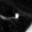
\includegraphics[width=\linewidth]{figures/heatmaps/ex1/sample_original.png}
        \caption*{Original 1}
    \end{subfigure}
    \begin{subfigure}[b]{0.18\textwidth}
        \centering
        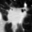
\includegraphics[width=\linewidth]{figures/heatmaps/ex2/sample_original.png}
        \caption*{Original 2}
    \end{subfigure}
    \begin{subfigure}[b]{0.18\textwidth}
        \centering
        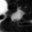
\includegraphics[width=\linewidth]{figures/heatmaps/ex3/sample_original.png}
        \caption*{Original 3}
    \end{subfigure}
    \begin{subfigure}[b]{0.18\textwidth}
        \centering
        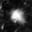
\includegraphics[width=\linewidth]{figures/heatmaps/ex4/sample_original.png}
        \caption*{Original 4}
    \end{subfigure}
    \begin{subfigure}[b]{0.18\textwidth}
        \centering
        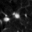
\includegraphics[width=\linewidth]{figures/heatmaps/ex5/sample_original.png}
        \caption*{Original 5}
    \end{subfigure}

    \vspace{2mm}

    % Second row: Fused model heatmaps
    \begin{subfigure}[b]{0.18\textwidth}
        \centering
        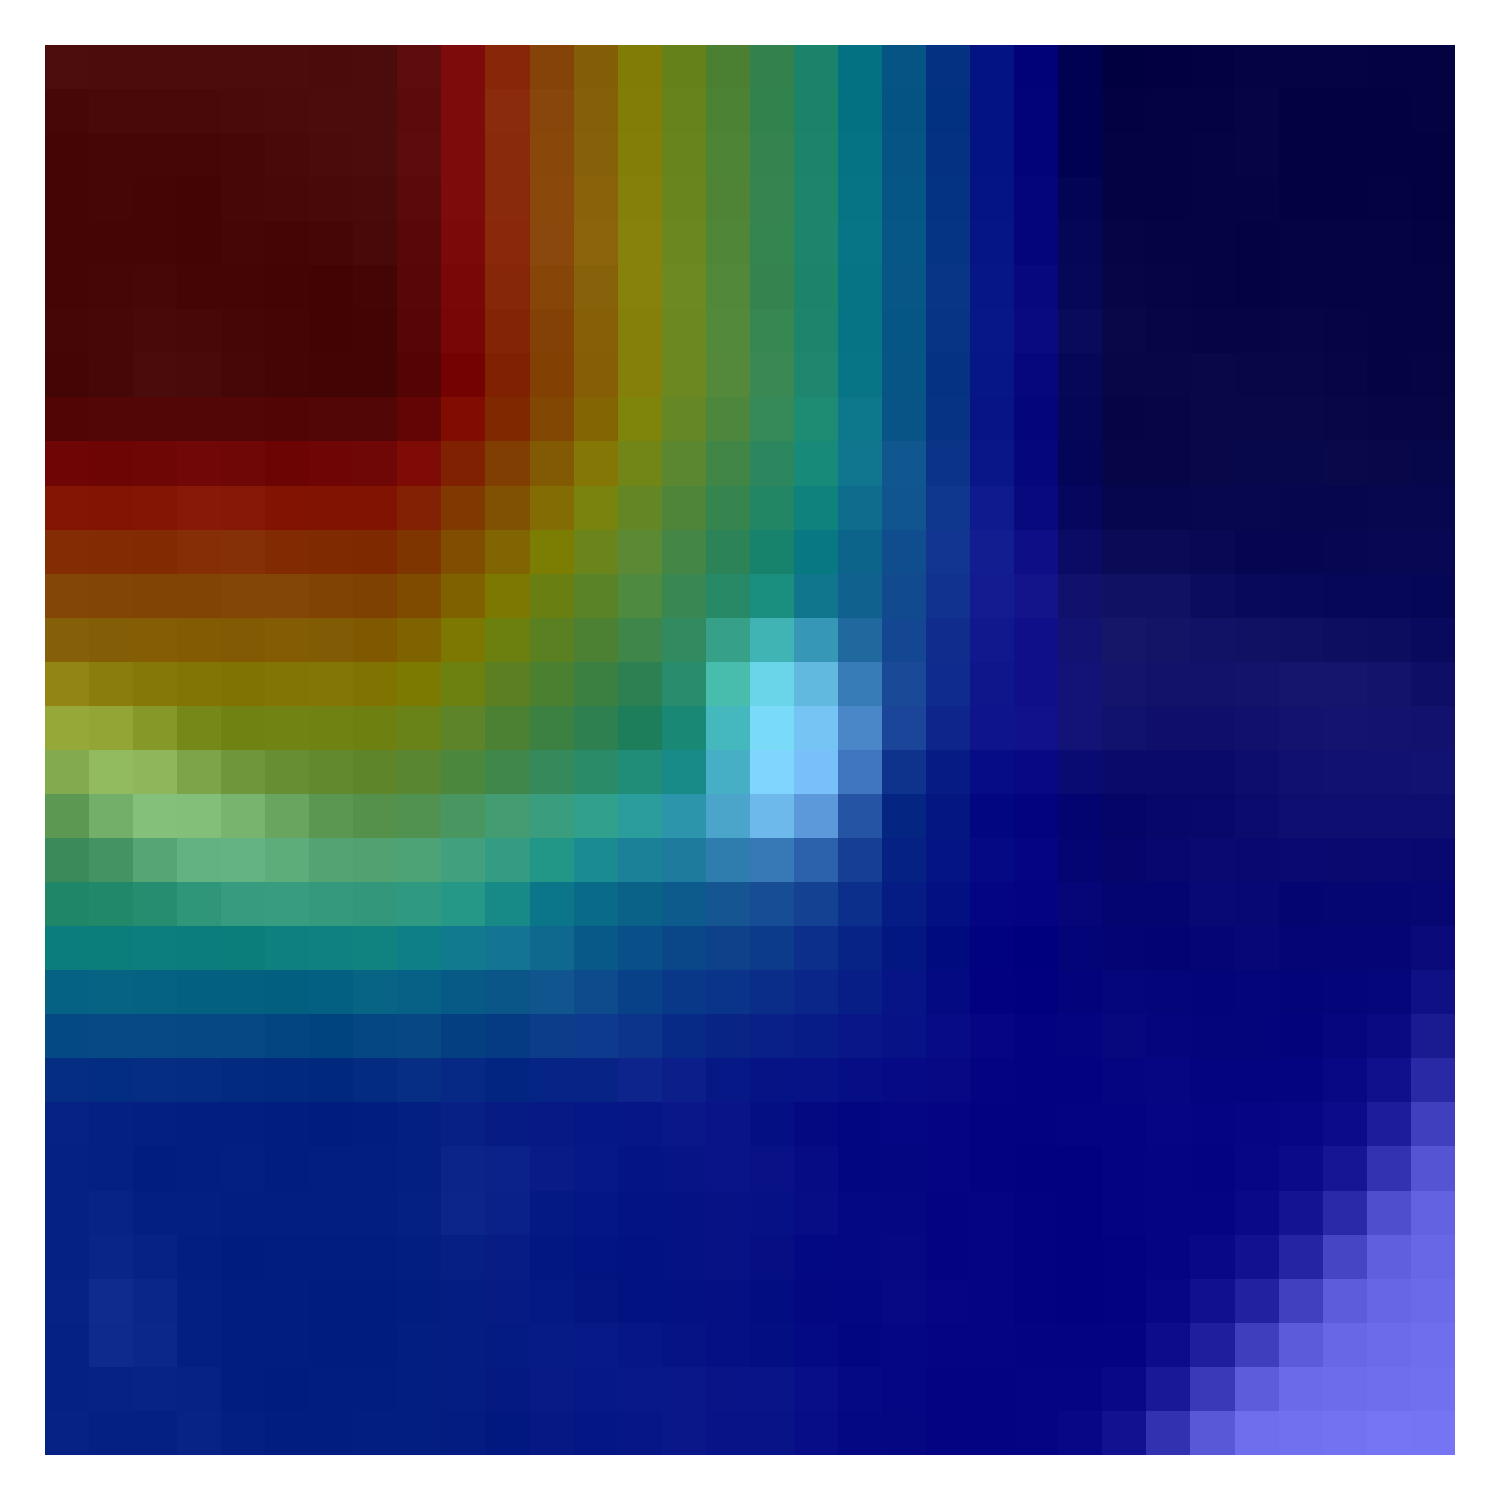
\includegraphics[width=\linewidth]{figures/heatmaps/ex1/sample_gradcam.png}
        \caption*{Fused 1}
    \end{subfigure}
    \begin{subfigure}[b]{0.18\textwidth}
        \centering
        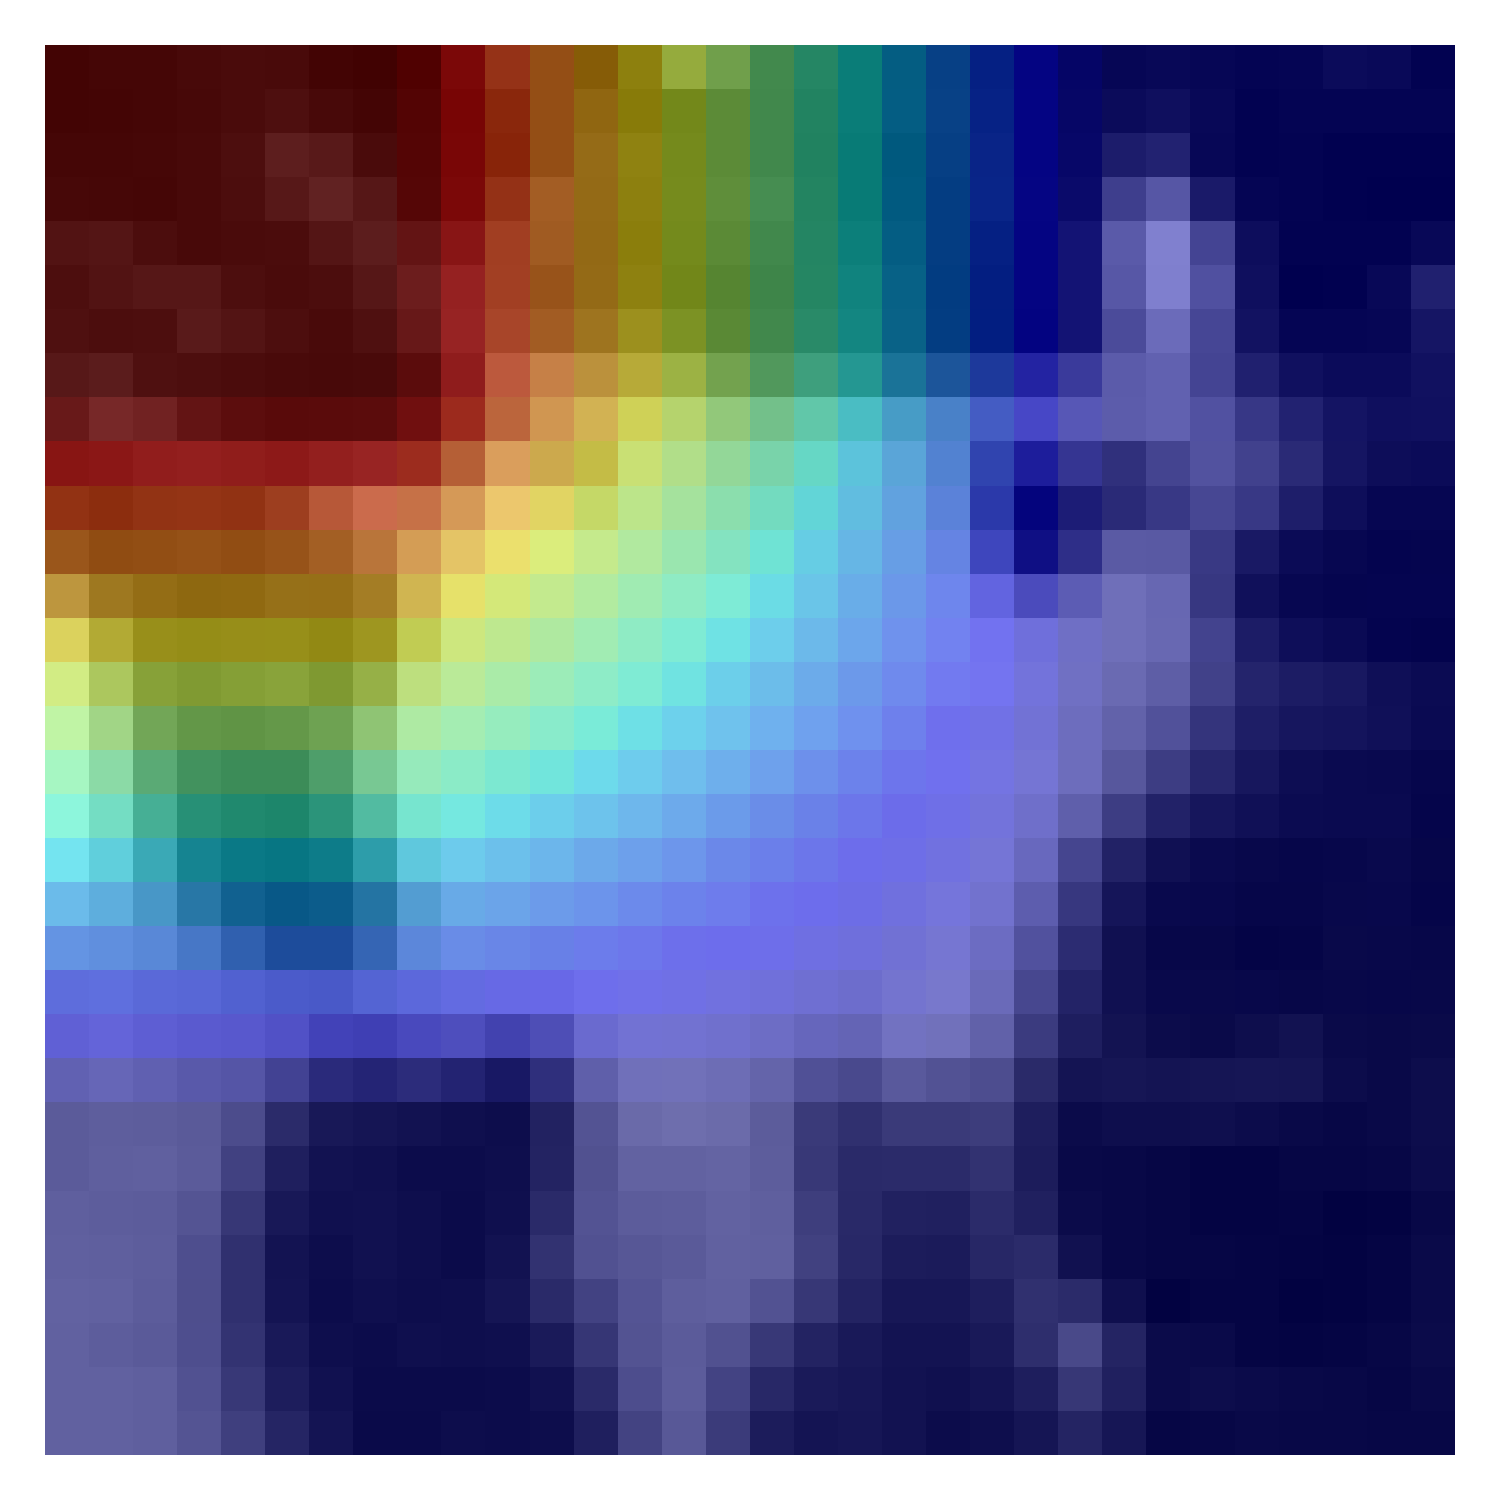
\includegraphics[width=\linewidth]{figures/heatmaps/ex2/sample_gradcam.png}
        \caption*{Fused 2}
    \end{subfigure}
    \begin{subfigure}[b]{0.18\textwidth}
        \centering
        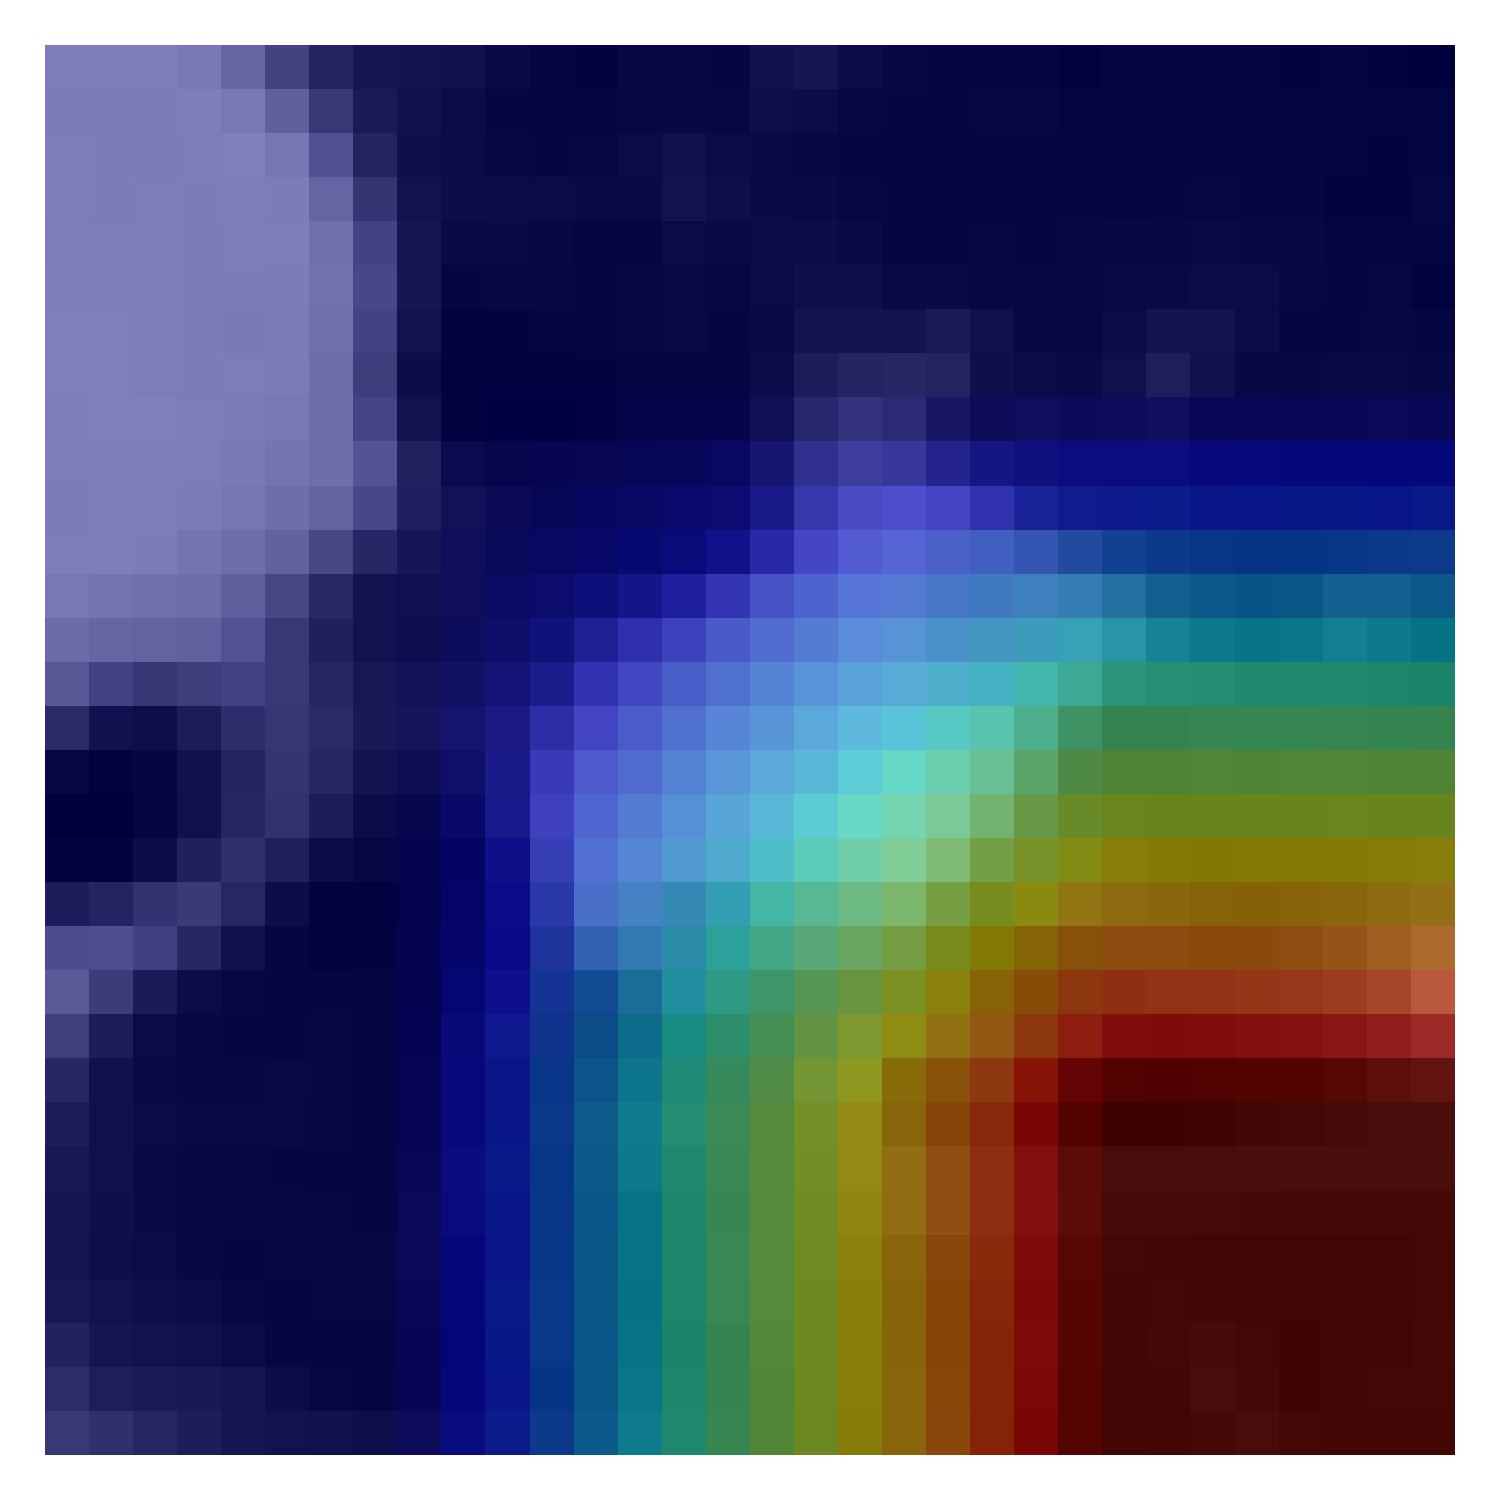
\includegraphics[width=\linewidth]{figures/heatmaps/ex3/sample_gradcam.png}
        \caption*{Fused 3}
    \end{subfigure}
    \begin{subfigure}[b]{0.18\textwidth}
        \centering
        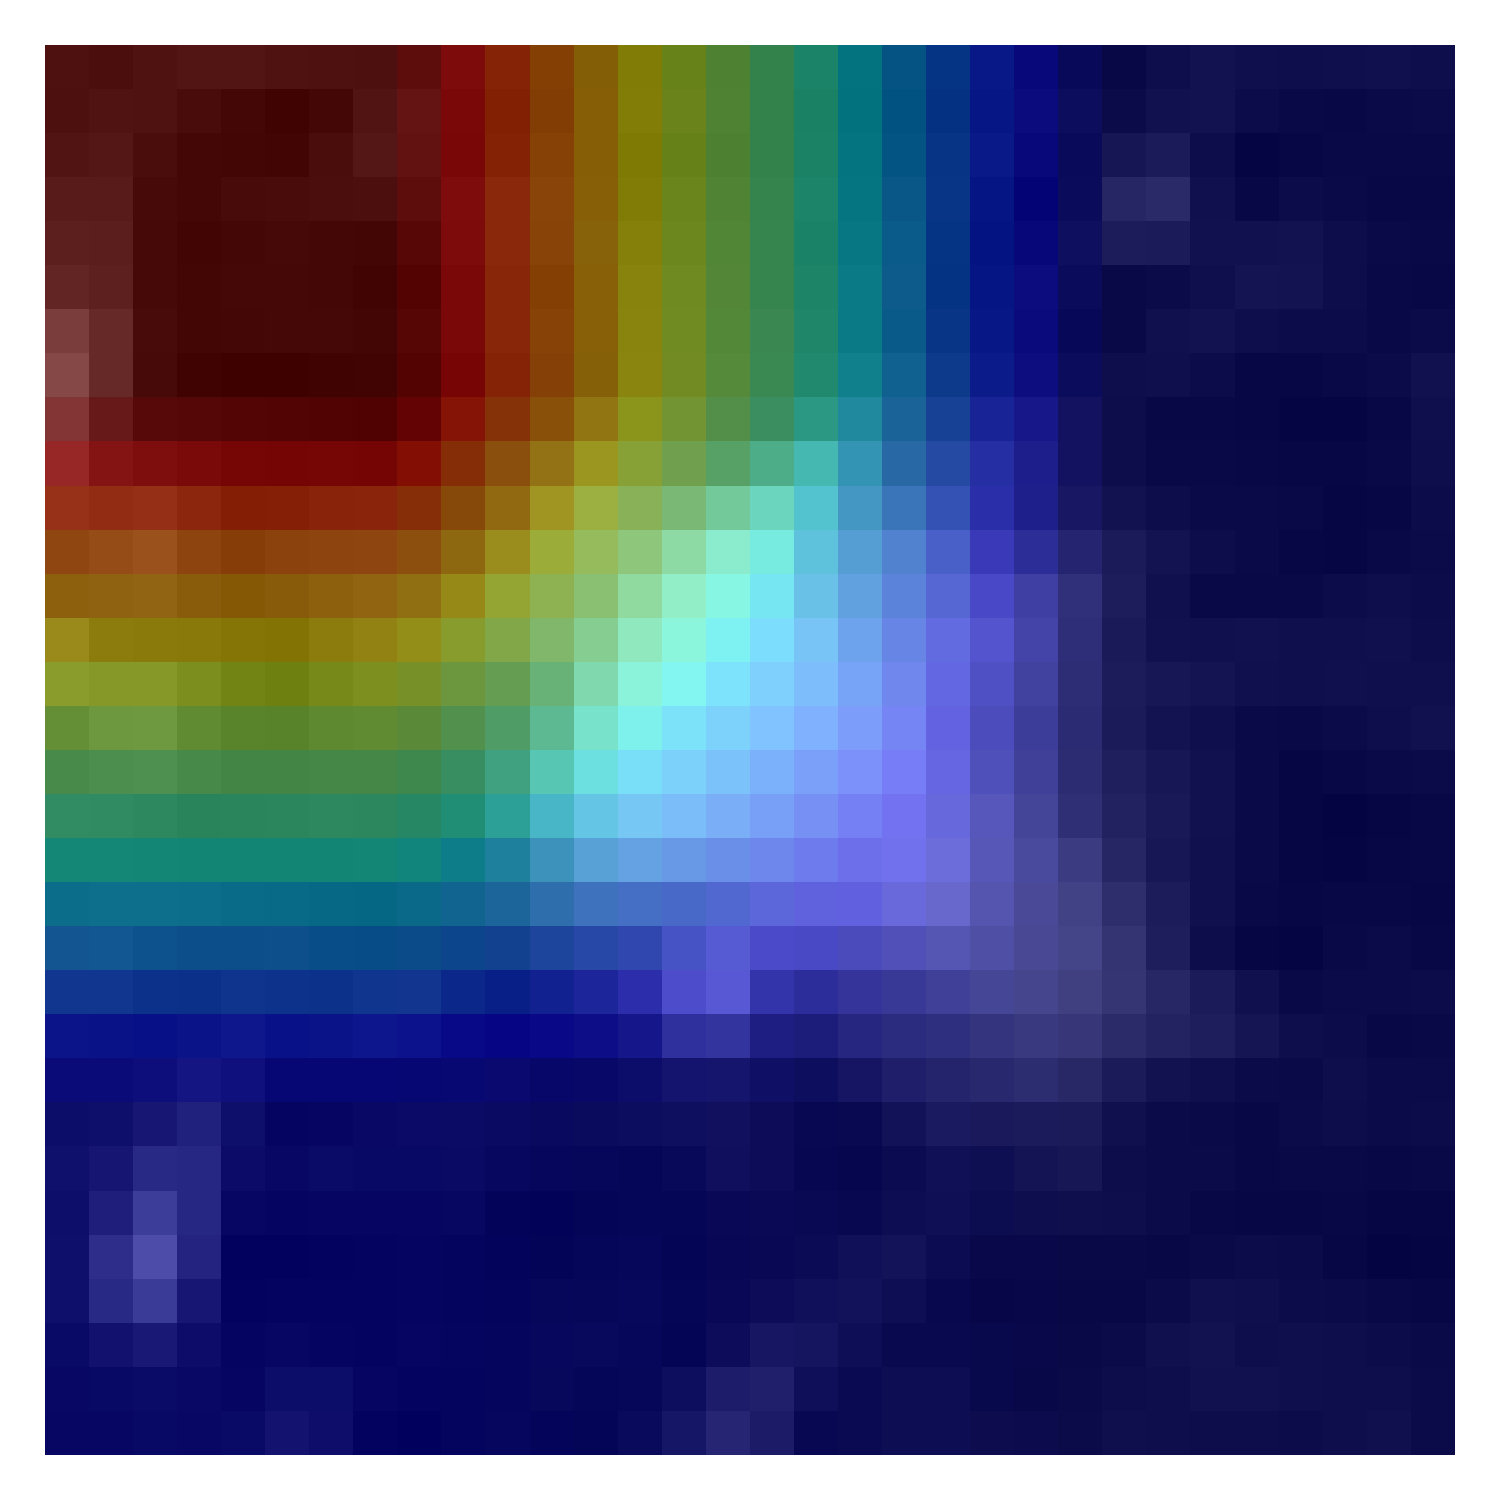
\includegraphics[width=\linewidth]{figures/heatmaps/ex4/sample_gradcam.png}
        \caption*{Fused 4}
    \end{subfigure}
    \begin{subfigure}[b]{0.18\textwidth}
        \centering
        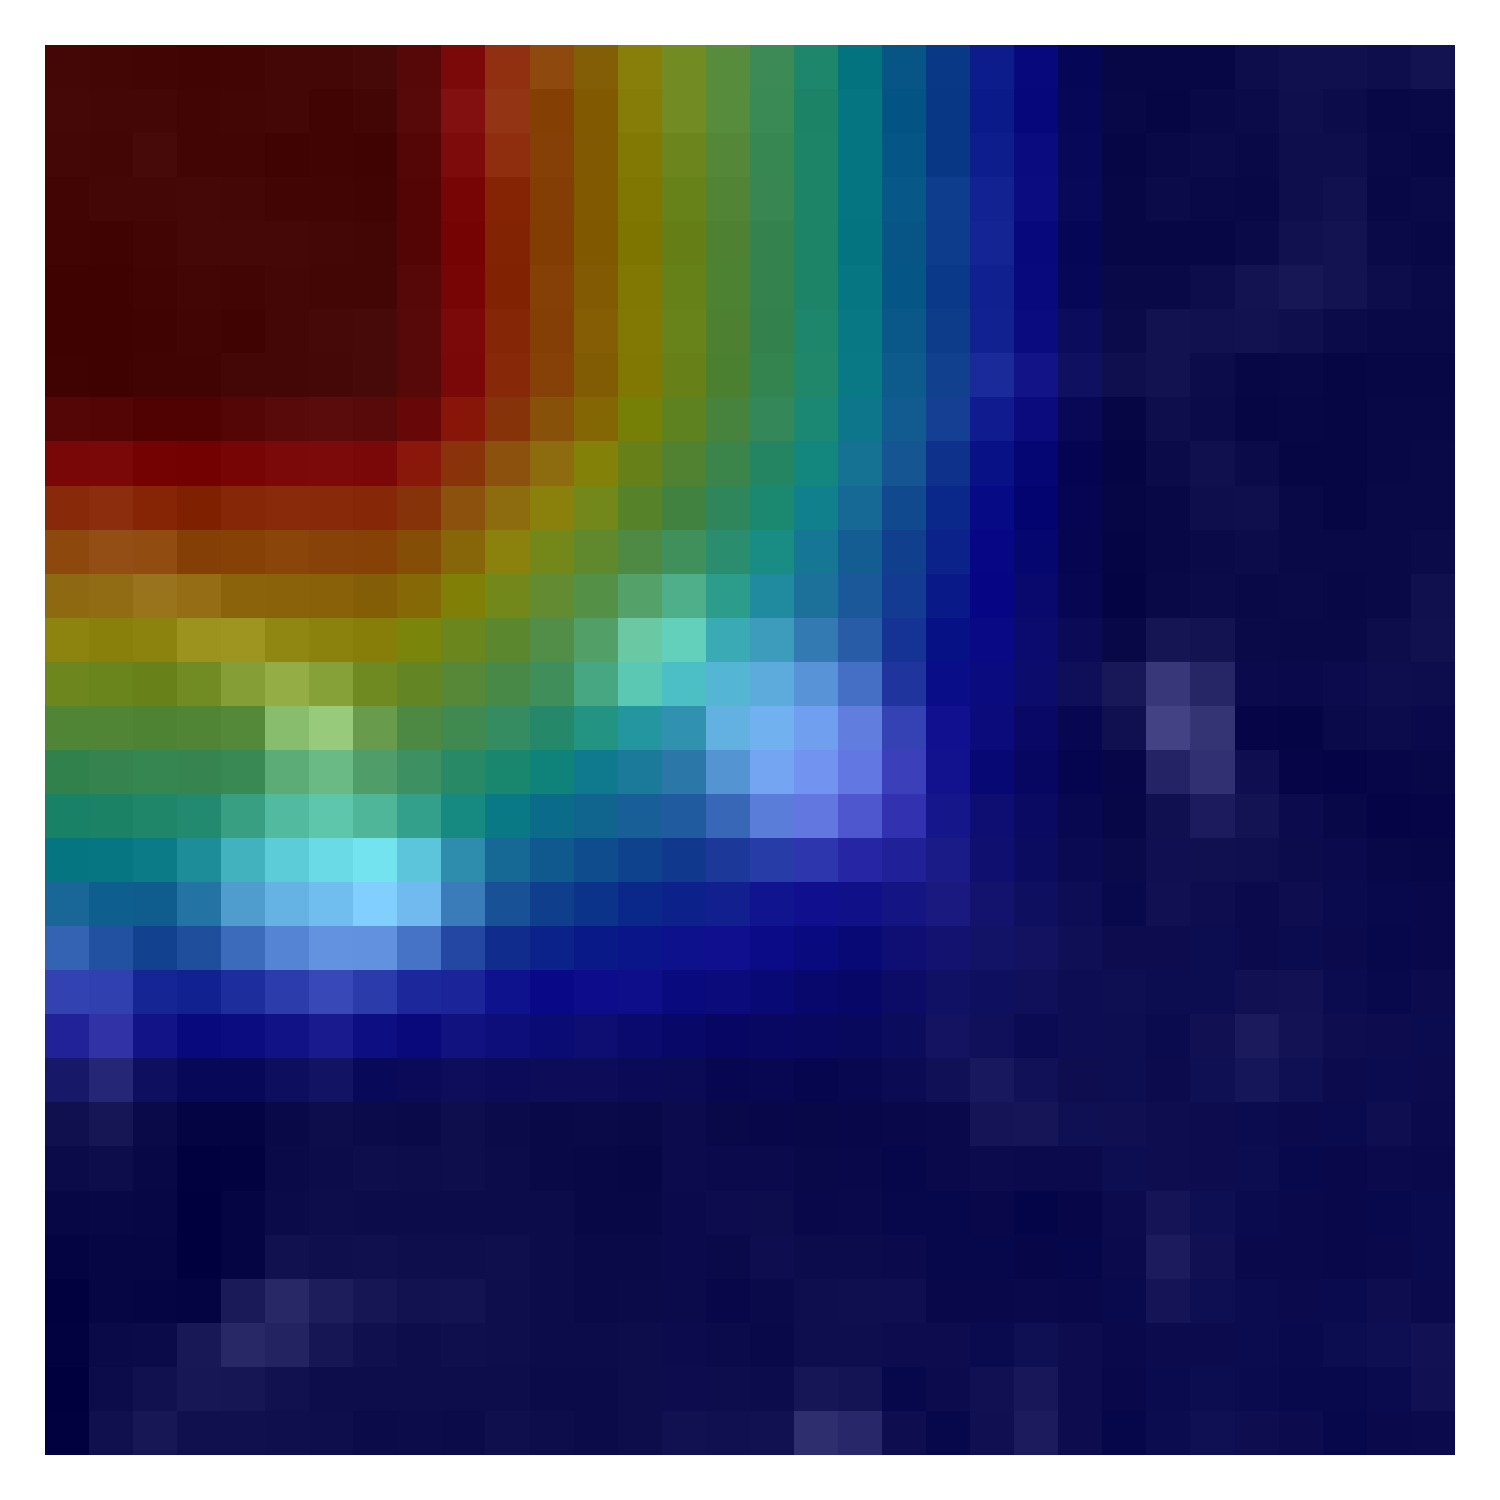
\includegraphics[width=\linewidth]{figures/heatmaps/ex5/sample_gradcam.png}
        \caption*{Fused 5}
    \end{subfigure}

    \vspace{2mm}

    % Third row: Non-Fused model heatmaps
    \begin{subfigure}[b]{0.18\textwidth}
        \centering
        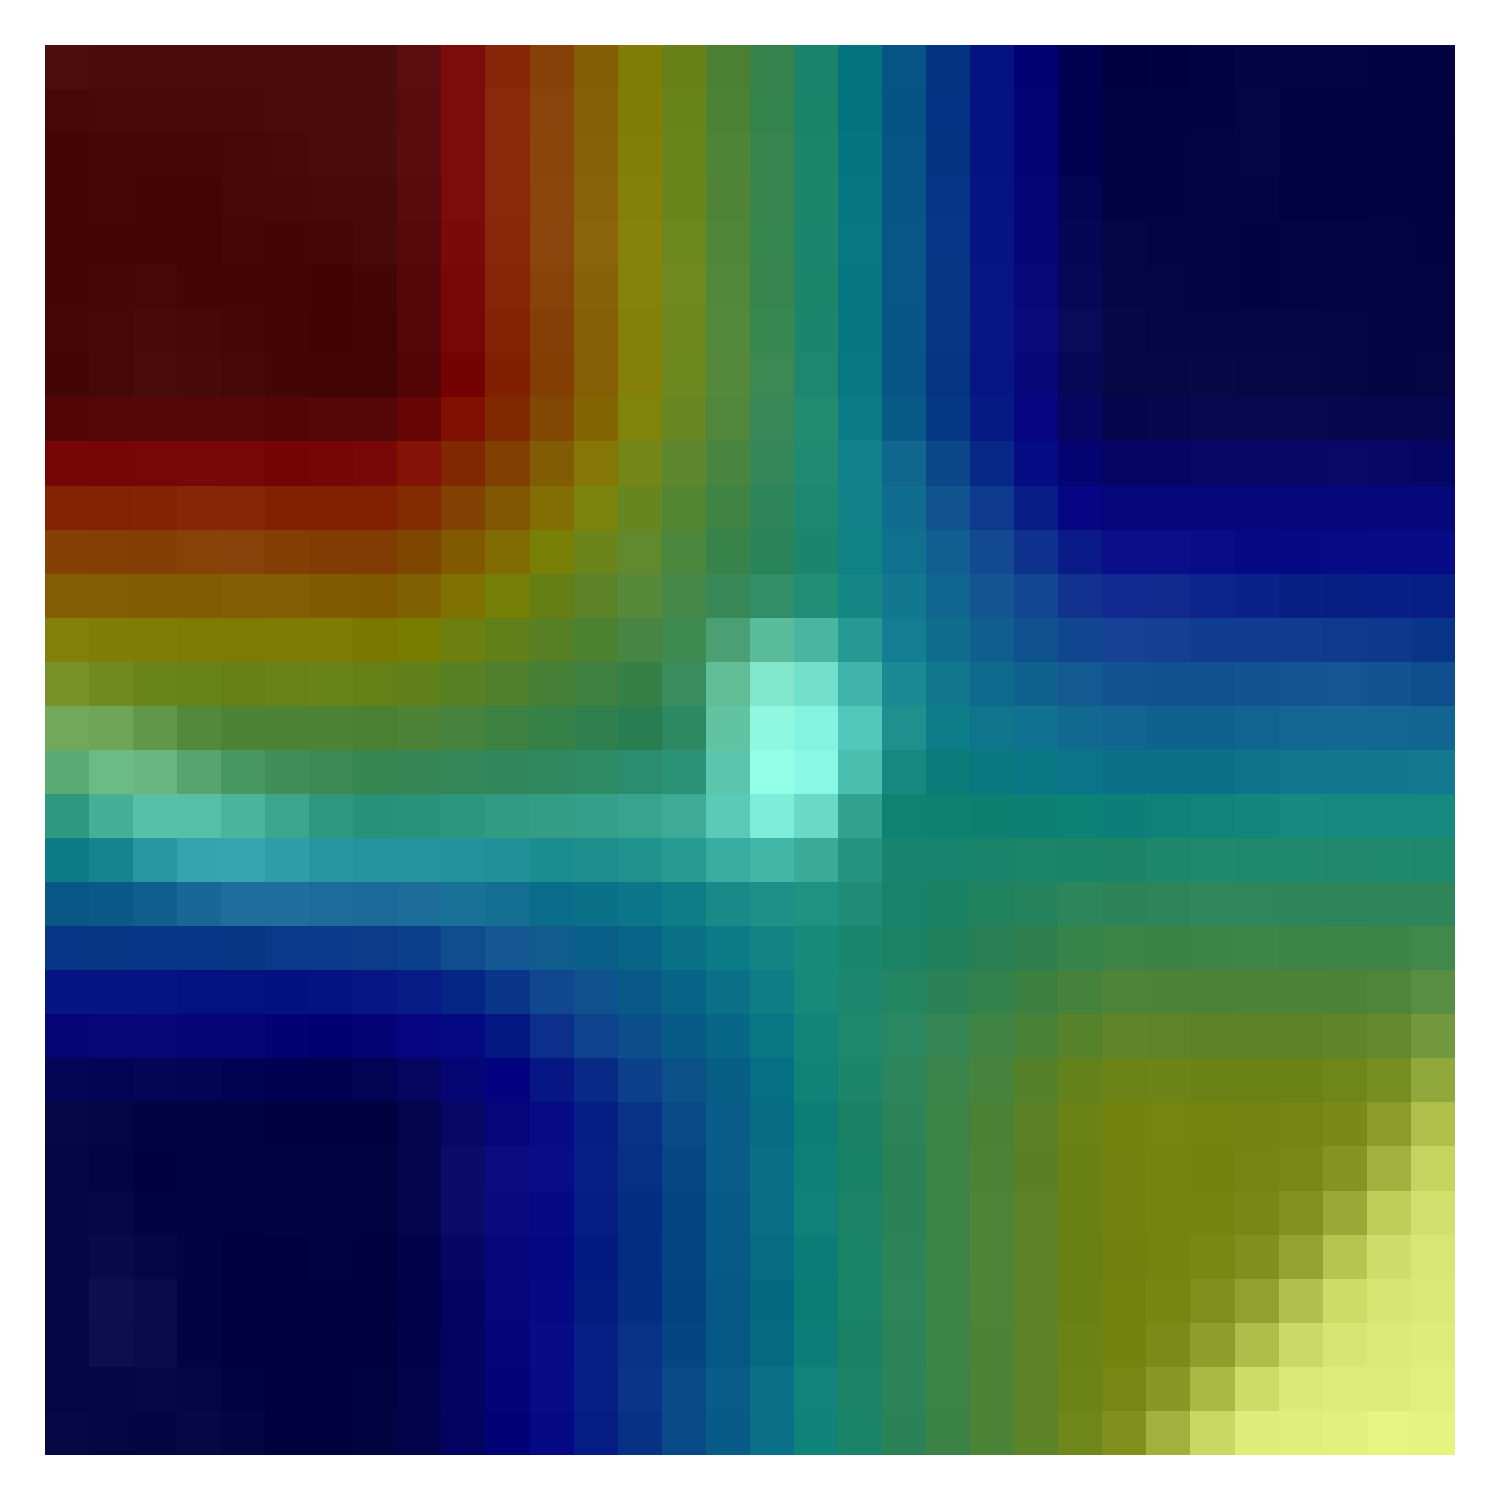
\includegraphics[width=\linewidth]{figures/heatmaps/ex1/sample_gradcam_non_fused.png}
        \caption*{Non-Fused 1}
    \end{subfigure}
    \begin{subfigure}[b]{0.18\textwidth}
        \centering
        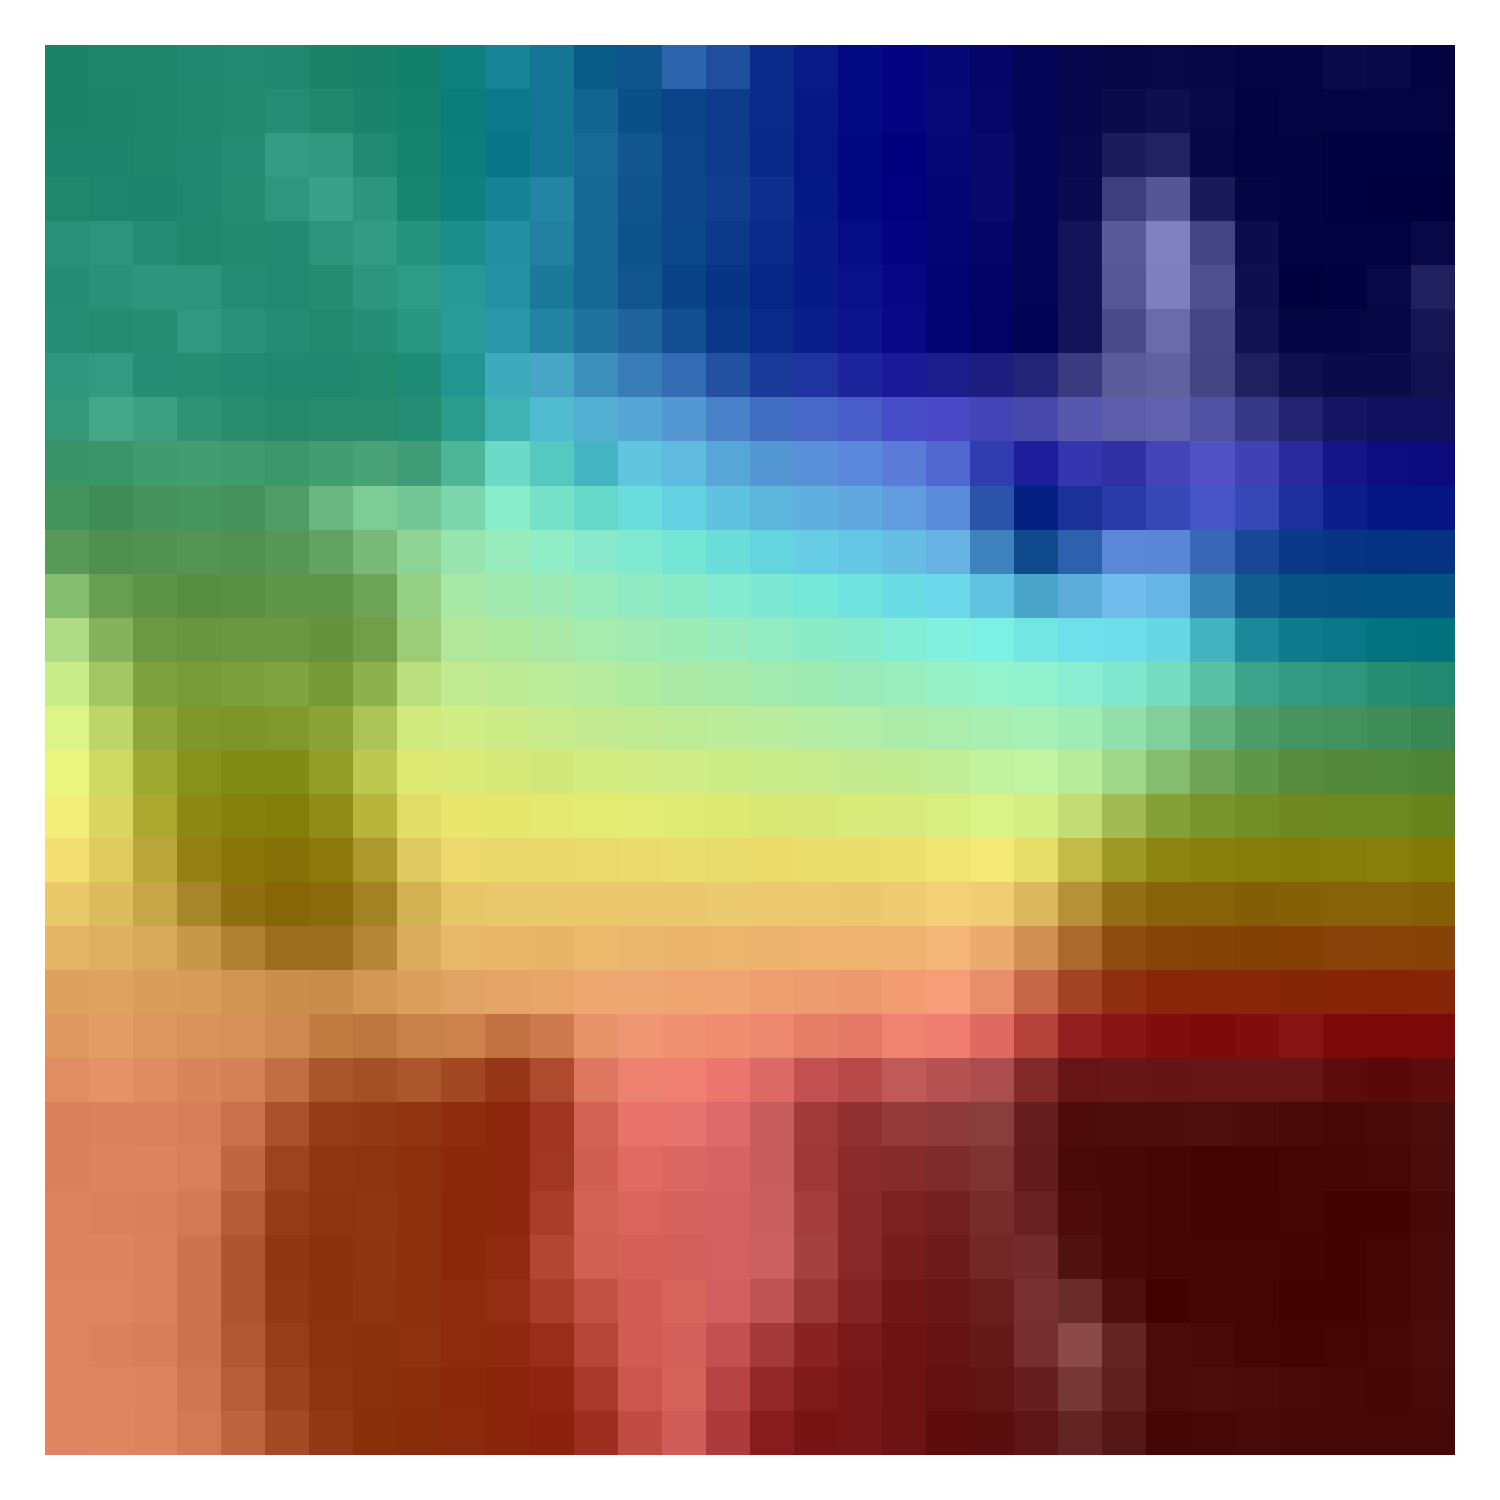
\includegraphics[width=\linewidth]{figures/heatmaps/ex2/sample_gradcam_non_fused.png}
        \caption*{Non-Fused 2}
    \end{subfigure}
    \begin{subfigure}[b]{0.18\textwidth}
        \centering
        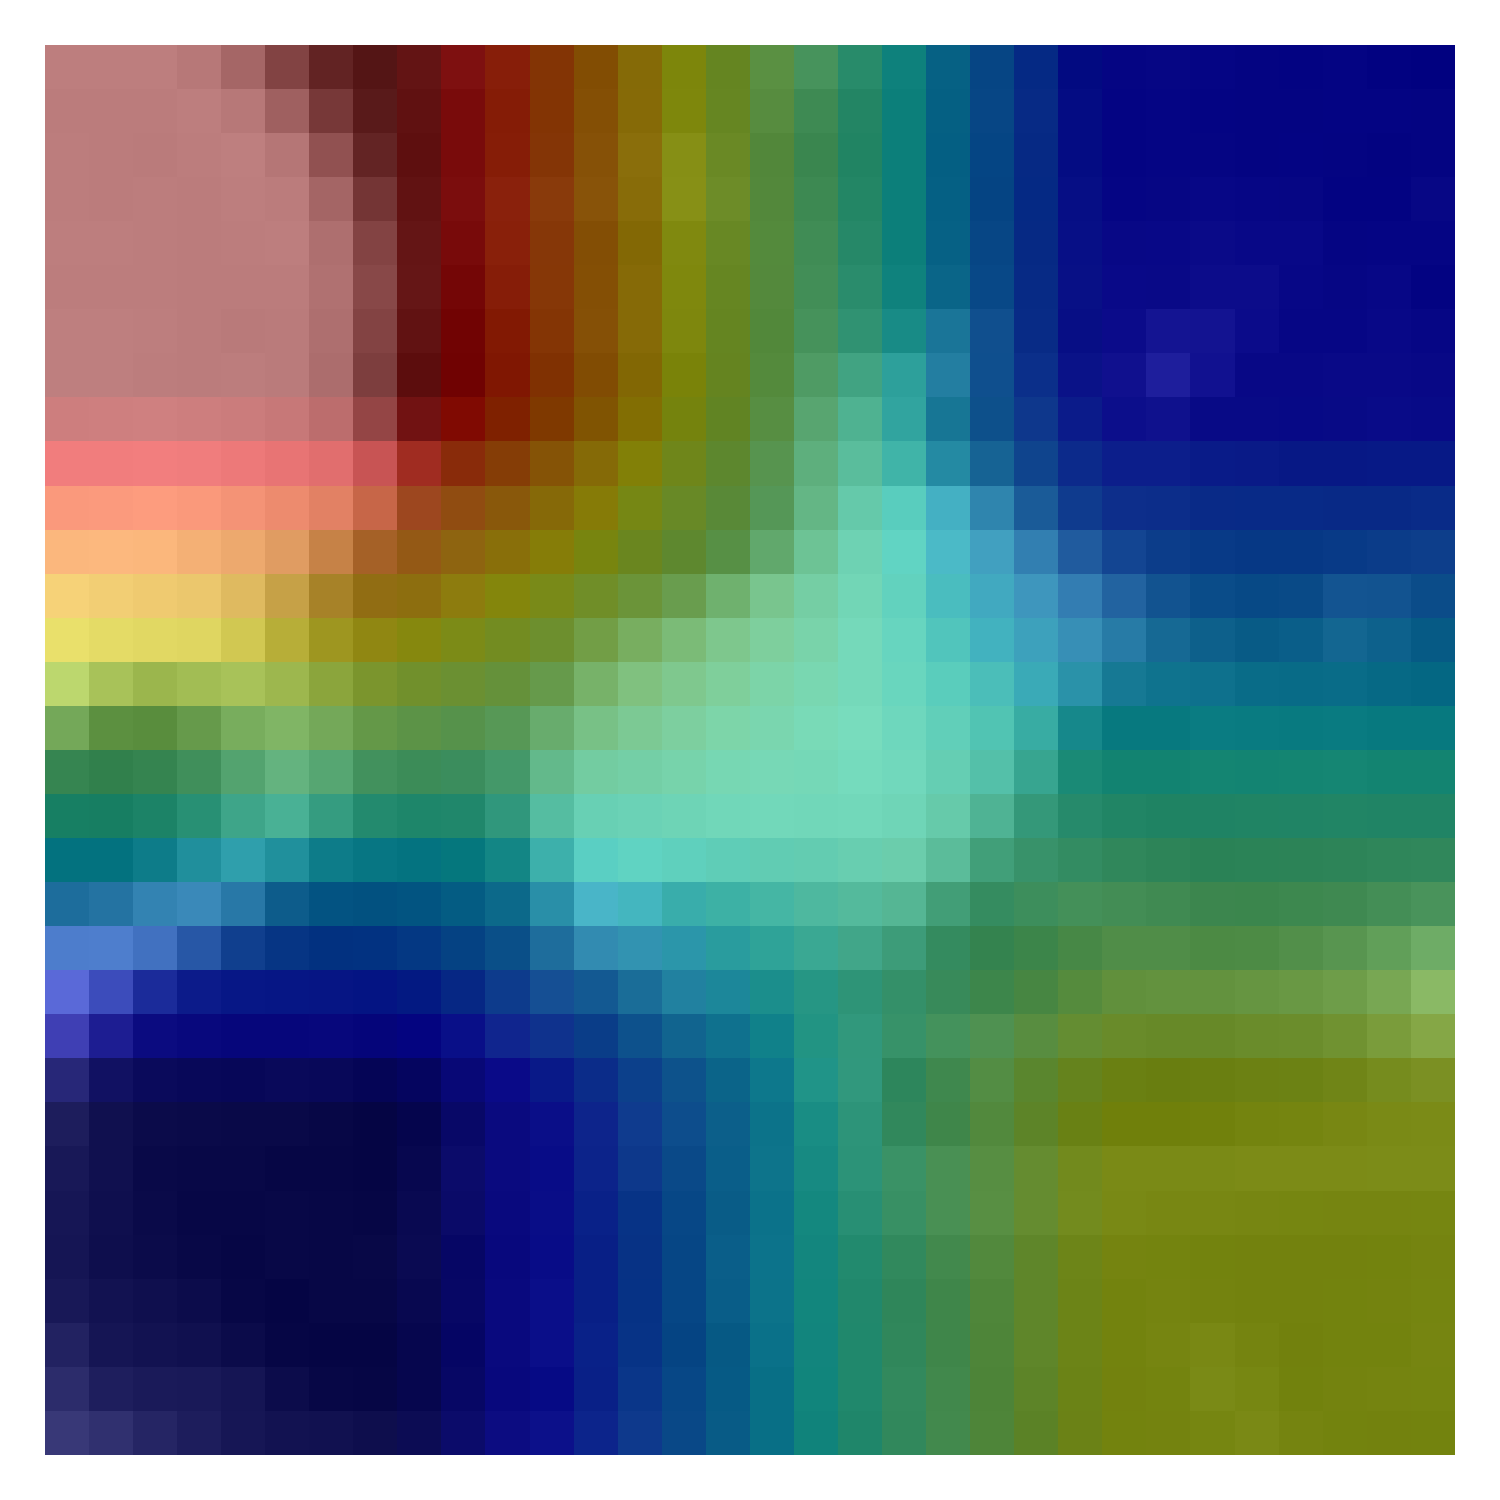
\includegraphics[width=\linewidth]{figures/heatmaps/ex3/sample_gradcam_non_fused.png}
        \caption*{Non-Fused 3}
    \end{subfigure}
    \begin{subfigure}[b]{0.18\textwidth}
        \centering
        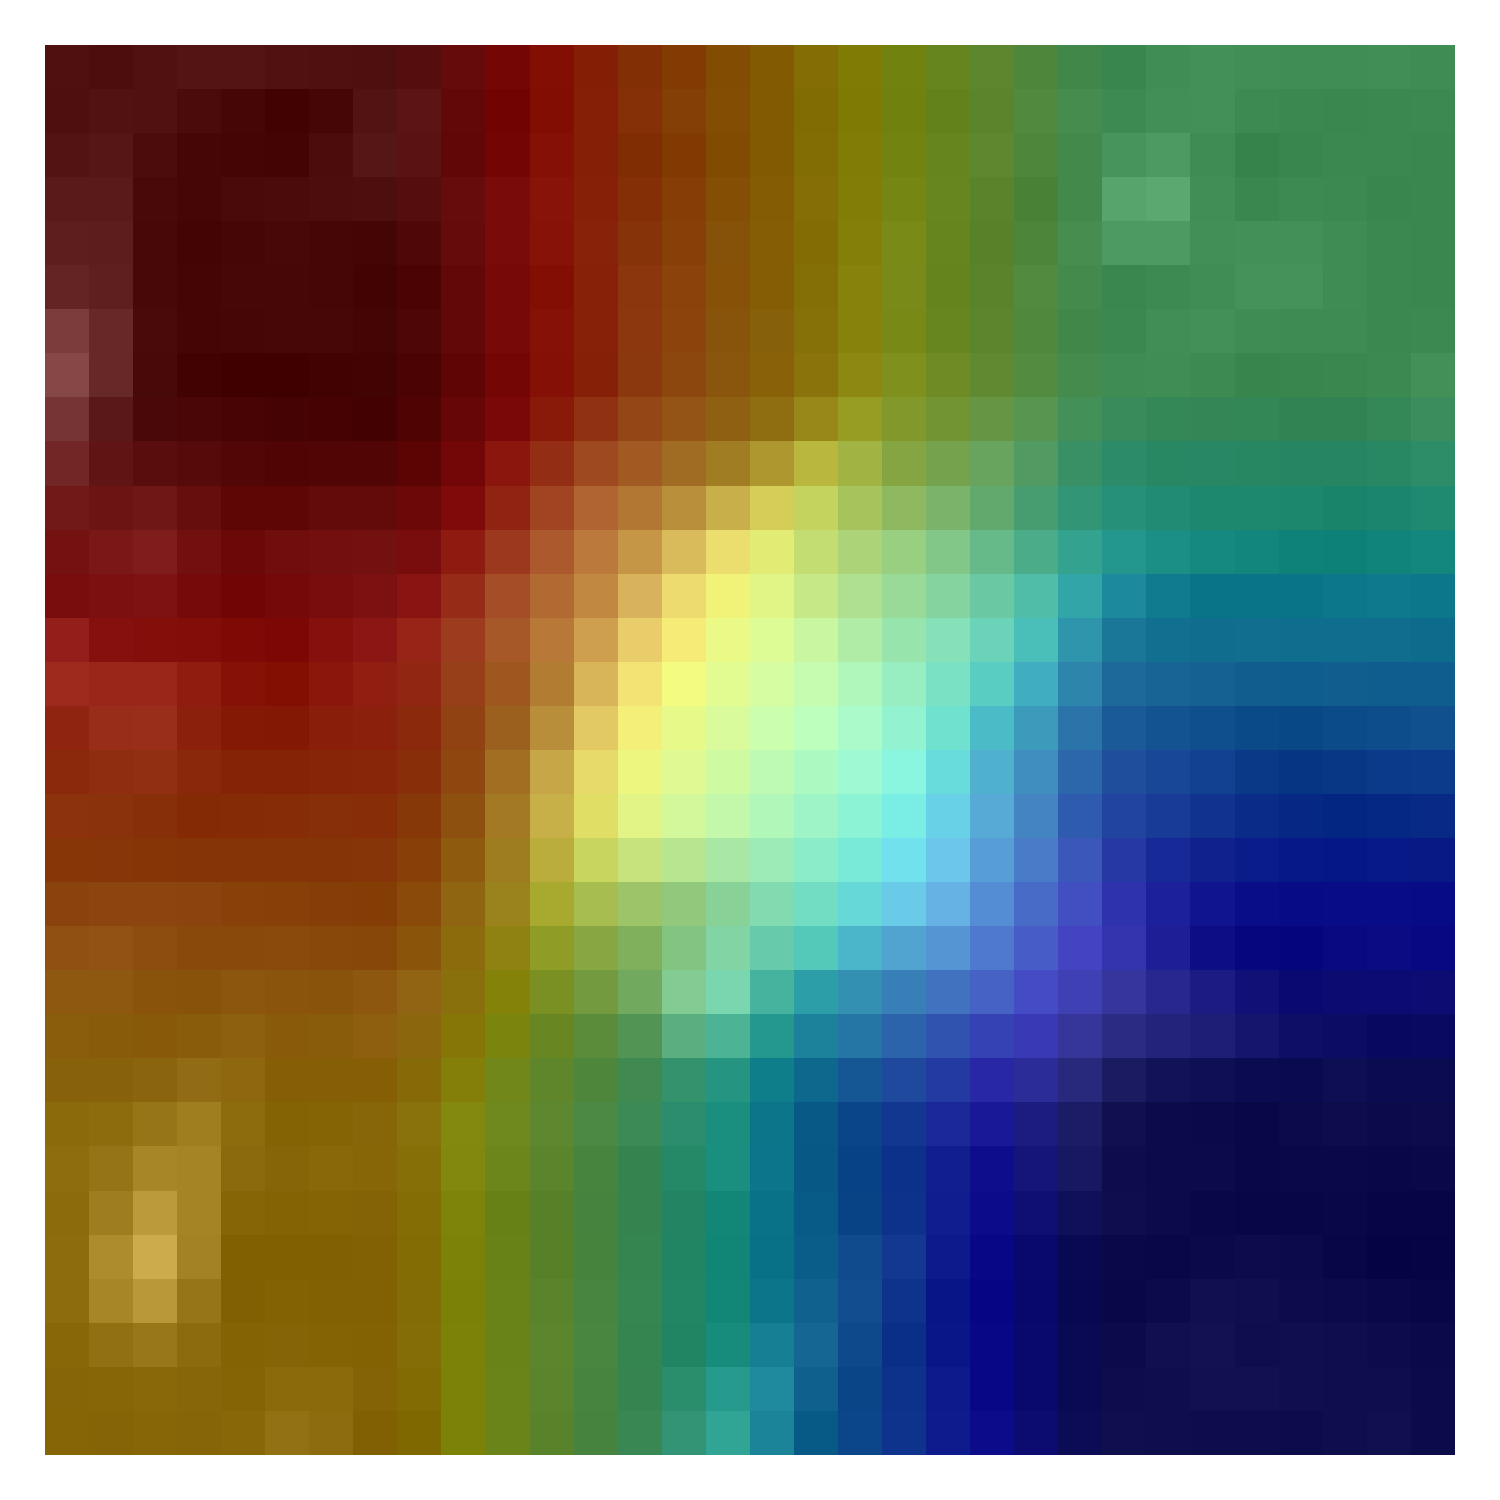
\includegraphics[width=\linewidth]{figures/heatmaps/ex4/sample_gradcam_non_fused.png}
        \caption*{Non-Fused 4}
    \end{subfigure}
    \begin{subfigure}[b]{0.18\textwidth}
        \centering
        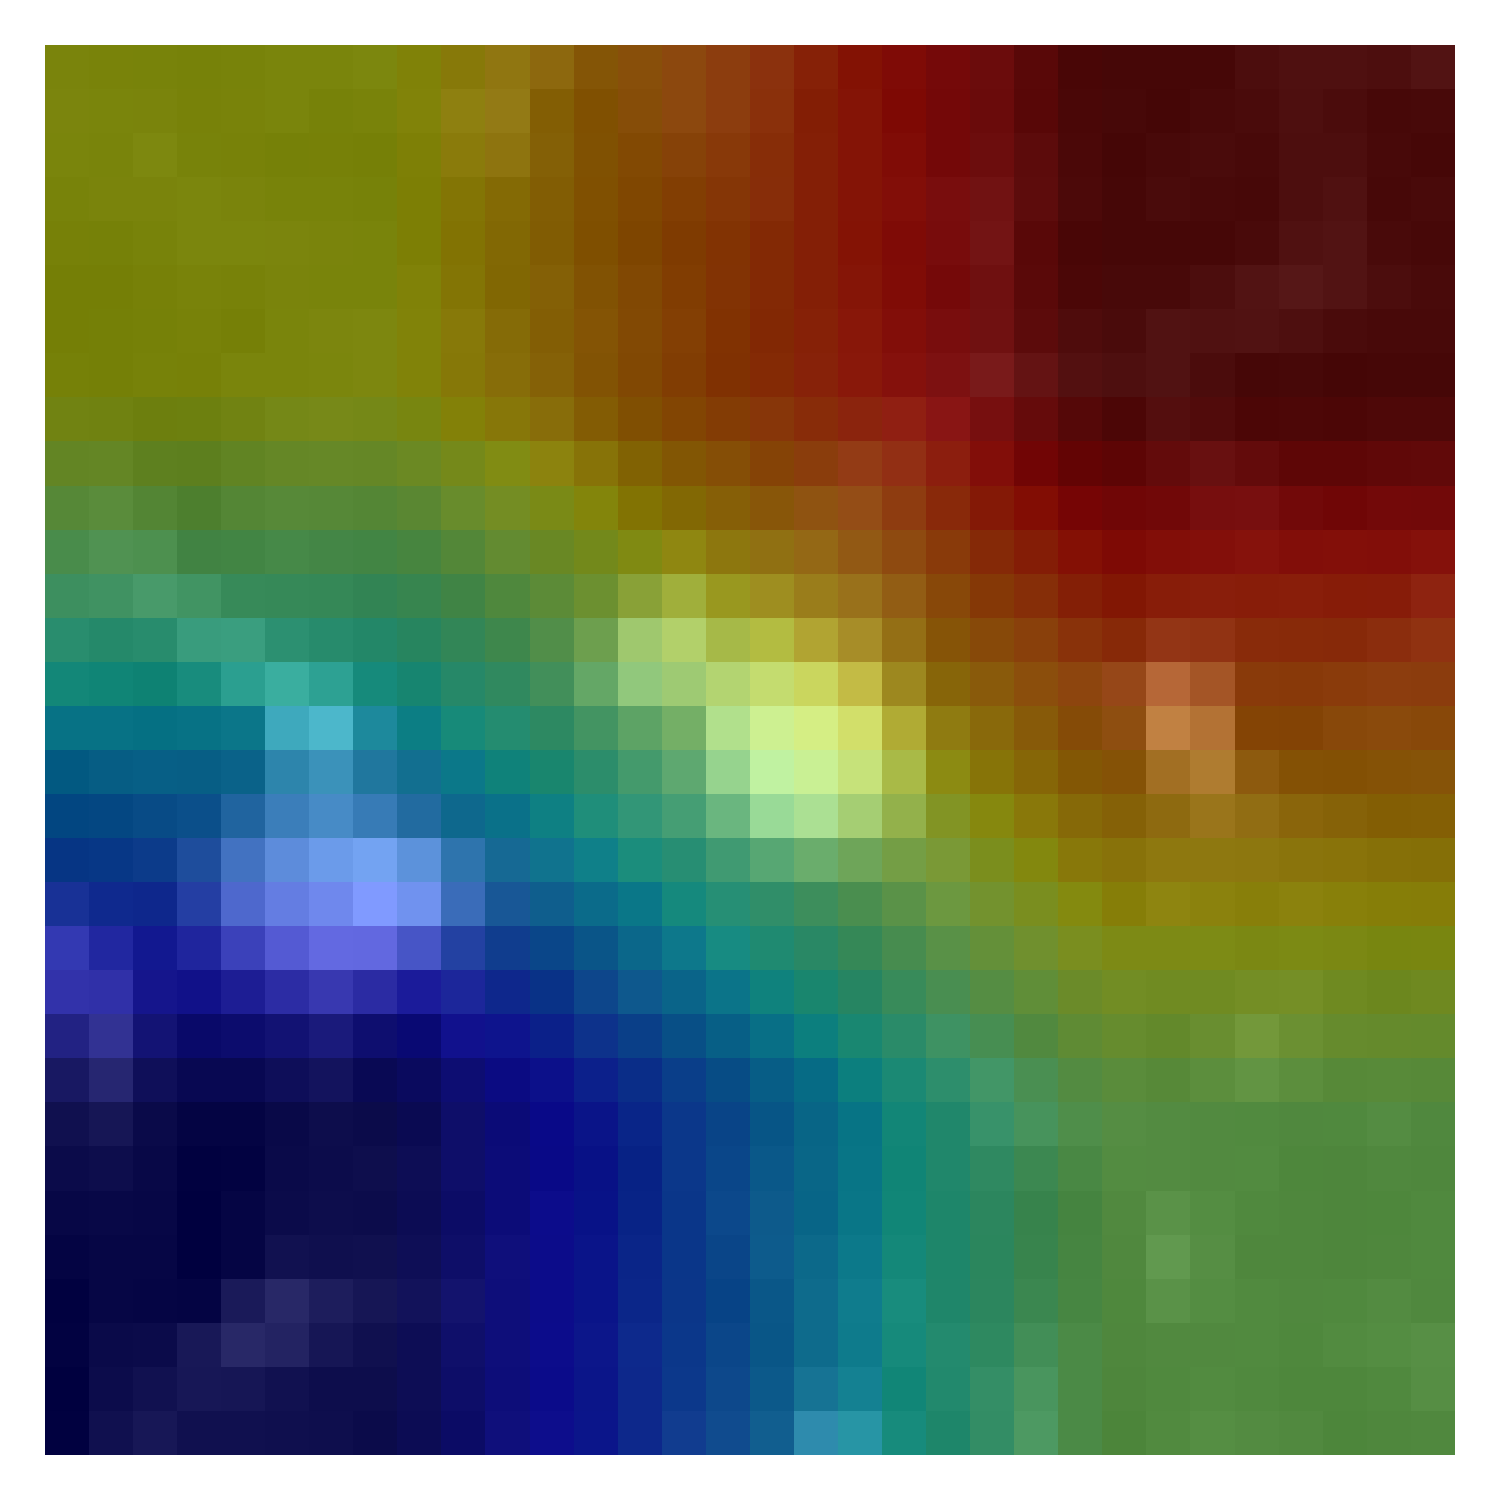
\includegraphics[width=\linewidth]{figures/heatmaps/ex5/sample_gradcam_non_fused.png}
        \caption*{Non-Fused 5}
    \end{subfigure}

    \caption[Grad-CAM Heatmap Comparison]{Comparison of Grad-CAM Heatmaps for five samples: Original images (top row), Fused model (middle row), and Non-Fused model (bottom row).}
    \label{fig:heatmap_grid}
\end{figure}


\subsection{SHAP}

\begin{figure}[htbp]
    \centering
    \begin{subfigure}[b]{0.45\textwidth}
        \centering
        \includegraphics[width=\linewidth]{figures/shap/true_positive/combined_shap_summary.png}
        \caption{True Positive}
    \end{subfigure}
    \begin{subfigure}[b]{0.45\textwidth}
        \centering
        \includegraphics[width=\linewidth]{figures/shap/false_positive/combined_shap_summary.png}
        \caption{False Positive}
    \end{subfigure}
    \vskip\baselineskip
    \begin{subfigure}[b]{0.45\textwidth}
        \centering
        \includegraphics[width=\linewidth]{figures/shap/false_negative/combined_shap_summary.png}
        \caption{False Negative}
    \end{subfigure}
    \begin{subfigure}[b]{0.45\textwidth}
        \centering
        \includegraphics[width=\linewidth]{figures/shap/true_negative/combined_shap_summary.png}
        \caption{True Negative}
    \end{subfigure}
    \caption[Local SHAP Analyses]{Local \ac{shap} Analyses for images representative of confusion matrix categories.}
    \label{fig:shap_analysis}
\end{figure}

Notably, \ac{shap} offers local, case-specific explanations, clarifying not only which features are significant on average but also how they specifically affect individual prediction outcomes within the confusion matrix.
The findings from the \ac{shap} analysis, illustrated in Figure~\ref{fig:shap_analysis}, offer valuable insights into the influence of specific radiomics features on the predictions made by the fused ResNet model across the four categories of the confusion matrix.

The results were derived by summing the \ac{shap} values for each feature. Higher positive \ac{shap} values indicate a greater influence on positive predictions, while negative values indicate influence on negative predictions.

Across all categories, the shape feature vector emerges as the primary contributor to the model's decisions. For both true positives and false negatives, the \ac{shap} values associated with Shape are significantly positive, suggesting that the presence of shape-related characteristics strongly reinforces the model's prediction of the positive class.

In the cases of false positives and true negatives, the \ac{shap} values for the Shape are strongly negative, indicating that when the shape feature influences the model towards the negative class, it does so with conviction. In contrast, the \ac{fof} and \ac{lbp} exhibit much smaller contributions across all categories: \ac{fof} has a minimal impact, whereas \ac{lbp} plays a slightly more significant role in negative-class predictions. 

This analysis confirms that integrating radiomics features with deep learning is most effective when shape features are included, as they significantly influence model predictions. The \ac{shap} analysis demonstrates that incorporating shape features enhances both interpretability and predictive power. In contrast, the contributions of \ac{fof} and \ac{lbp} are modest, suggesting that while multi-feature fusion offers complementary insights, the primary benefit comes from shape information. 
\chapter{Conclusions}\label{chap:conclusions}

\section{Research Questions}


This work set out to answer three principal research questions:

\begin{enumerate}
  \item \textbf{Does fusing information from shallow and deep feature extractors improve classification or generalization performance compared to using a deep extractor?}\\
From all the experiments performed, we were able to identify robust evidence that fusing shallow radiomics features with deep neural representations leads to consistent improvements in both classification and generalization performance when compared to conventional standalone deep learning models.

The established base models - the families of ResNet and EfficientNet, along with ConvNeXt-Tiny, demonstrate an already competitive performance on the LIDC-IDRI, defining a target to be surpassed by fused models. The fact that lighter architectures match or even outperform deeper counterparts, such as EfficientNet-B0 and ResNet-18, respectively, suggests that merely increasing network depth or complexity would result in diminishing returns for this specific domain.

For example, combining Shape, \ac{lbp}, and \ac{fof} features at empirically optimal points in ResNet-18 led to an improvement in \ac{auc} from 0.82 to 0.86, along with a notable increase in accuracy, precision, and sensitivity compared to the baseline, as shown in Table~\ref{tab:resnet18_fusion_metrics}.

Notably, most effective gains were observed when complementary radiomics features were fused, indicating the existence of synergy in combining diverse shallow descriptors with hierarchical deep features. In particular, with the 2D Shape descriptors, this synergy consistently contributed to the most significant performance boost; however, combinations of two or three features performed better than any individual feature when fused.

The benefits of fusion generalization are evident in the stability of performance improvements, which remain consistent across variations in model hyperparameters and fused blocks (Tables~\ref{tab:fof_hyperparam}--\ref{tab:2dshape_hyperparam}).
Most of the optimal fusion occurred at earlier ResNet blocks, suggesting that shallow features can be most effective when complementing deep representations before excessive abstraction. 

In summary, these results underscore that carefully designed fusion could lead to improvements in state-of-the-art shallow and deep-only approaches.

  
  \item \textbf{How does the fusion approach behave under varying dataset conditions, such as different sample sizes, bounding‐box definitions, and image representations?}\\
The ablation study conducted—detailed in Table~\ref{tab:resnet18_vs_fused}—investigated how the Fused model and its corresponding Baseline performed under various conditions. Across all scenarios, the fusion solution demonstrated superior performance, with the exception of sensitivity in the Central Scores case where it matches. However, the magnitude of its improvements was influenced by the complexity and representation of the subsets presented.

The results indicate that the auxiliary information derived from radiomics features is particularly valuable in challenging classification scenarios, where deep models alone may struggle to capture subtle and discriminative cues.

Importantly, fusion retained its advantage even as the nature of the input data changed. Suggesting that shallow features encode information orthogonal to that of deep network representations, and that their integration is beneficial across diverse imaging resolutions and multi-view data. 

Collectively, these findings indicate that the fusion approach is more robust and adaptable than the non-fused approach, capable of better generalizing across a range of clinical data conditions.
  
  \item \textbf{In what ways does information fusion contribute to the explainability of lung nodule malignancy predictions?}\\
Using Grad-CAM (Figure~\ref{fig:heatmap_grid}), we exhibited that the fused model generates \ac{cam} that exhibit more anatomically relevant attention, centralizing on nodule regions and boundaries. In contrast, the non-fused model tended to show a more diffuse or background-oriented focus. This suggests that the incorporation of shallow features assists in directing the model’s attention toward appropriate clinical structures, proposing more trustworthy and easier decisions for clinicians to interpret.

The \ac{shap} analyses (Figure~\ref{fig:shap_analysis}) offer additional insights by quantifying the influence of each radiomics feature vector on individual predictions. \ac{shap} revealed that the 2D Shape feature positively affects true positives and false negatives, while negatively impacting true negatives and false positives, always leaning towards the correct decision. The other tested features, \ac{fof} and \ac{lbp}, contribute in a complementary, but less pronounced manner.
This direct correlation between radiomics descriptors and model outputs facilitates interpretations that coincide with medical reasoning, thereby contributing to the improvement in transparency.

The improvements in interpretability are not simply coincidental, since they are a direct outcome of the fusion process. The rationale behind the model becomes more transparent and easier to audit by systematically integrating features that have clear clinical relevance.
\end{enumerate}

\section{Hypothesis}

Based on our research and previously analysed research questions, the fusion paradigm between complementary types of features yields higher predictive capability. This statement is supported by tangible improvements in \ac{auc}, accuracy, precision, and sensitivity across all tested architectures over each respective baseline.
The most significant gains were achieved when multiple handcrafted features were injected, after an optimal block, supporting the hypothesis of enhanced model performance.

The higher adaptability was also observed across different sets of data. Since in all data cases the fused model surpassed or matched the non-fused one, with the most significant disparities in more ambiguous or complex data subsets.
These exhibits indicate that the fusion approach could be better, more robust, and more adaptable, further validating its reliability for diverse clinical scenarios.
Information fusion is essential for enhancing advanced deep classifiers when they either reach a performance plateau or show decreased accuracy as their depth or complexity increases.

Additionally, we not only observed increments in quantitative metrics but also in interpretable relationships, as the fused model presented a less diffuse visualization. Additionally, the fused features present a leaning towards the right decision, mainly observed with the Shape descriptor.
These findings address the need for more reliable and understandable diagnostic systems.

The evidence collected from this study strongly supports our hypothesis that the fusion of shallow and deep features provides a superior paradigm for the detection and diagnosis of lung nodules.
Fusion methods deliver gains in predictive performance, generalizability, interpretability, and adaptability, which are crucial for lung cancer diagnostics and for supporting real-world practice.


\section{Main Contributions}

This dissertation makes significant strides in the realm of \ac{cad} for lung cancer, highlighting several pivotal advancements:

\begin{itemize}
    \item \textbf{Development of a Fusion-Based Diagnostic Framework:} This research introduces a novel deep learning model that synergistically combines handcrafted radiomics features - such as shape, \ac{lbp}, and the \ac{fof} - with deep features derived from ResNet architectures. The integration of these diverse feature sets led to marked improvements in the model's classification accuracy compared to traditional baseline models, thereby enhancing diagnostic precision.

    \item \textbf{Systematic Evaluation of Fusion Strategies:} Through rigorous experimentation that spanned multiple stages of feature fusion and architectural variations, this work successfully identified the most effective fusion points, particularly at earlier layers of the network. These insights maximized the beneficial interactions between shallow and deep features, thus optimizing overall model performance.

    \item \textbf{Enhanced Explainability in \ac{ai}-Driven Diagnostics:} By employing advanced interpretability techniques such as Grad-CAM and \ac{shap}, the decision-making process of the model was rendered more transparent. This enhancement not only validated the importance of shape features in the diagnostic process but also fostered greater trust and confidence in the \ac{ai} 's predictive outputs among clinicians.

    \item \textbf{Empirical Validation Across Diverse Data Conditions:} The robustness of the proposed fusion approach was thoroughly validated under a variety of dataset conditions, encompassing different image representations, sizes, and bounding box strategies. This comprehensive examination underscored the framework's versatility and broad applicability in real-world scenarios.

    \item \textbf{Contribution to \ac{sdg} 3:} This research aligns with and advances \ac{sdg} 3, focusing on health and well-being. Creating non-invasive, interpretable, and accessible diagnostic tools contributes significantly to the early detection of lung cancer and promotes equitable access to healthcare resources.
\end{itemize}

\section{Future Work}

Building upon the foundation established for fusion-based lung nodule characterization, numerous intriguing avenues for future research have been identified:

\begin{itemize}
    \item \textbf{Application to 3D and Temporal Data:} Further development could involve transitioning from current 2D and 2.5D image representations to fully adapting 3D \ac{ct} volumes and longitudinal patient scans. This change would facilitate improved nodule characterization by leveraging the spatial nuances and temporal dynamics of lung nodules.

    \item \textbf{Automated Feature Selection and Optimization:} The exploration of implementing attention mechanisms or strategies for feature selection holds the promise of dynamically adjusting the weighting of features. This could significantly enhance the performance and generalizability of the fusion models.

    \item \textbf{Hyperparameter Tuning of Feature Extractors:} A systematic approach to hyperparameter optimization for each handcrafted feature extractor would likely yield improvements in the quality and discriminative power of the fused features, leading to better diagnostic outcomes.

    \item \textbf{Multi-Label Classification:} Investigating methods for multi-label classification could enable the model to predict multiple attributes or characteristics of a nodule simultaneously, encompassing features such as malignancy, calcification, and spiculation, thereby providing a more comprehensive diagnostic overview.

    \item \textbf{Clinical Validation and Deployment:} Engaging in collaboration with medical professionals to validate the model within real-world clinical environments is critical. This step would include its integration into existing radiology workflows to facilitate practical application and acceptance by the medical community.

    \item \textbf{Benchmarking Against Multicenter Datasets:} Conducting evaluations of the model across diverse datasets collected from multiple hospitals or geographic regions would serve to test its generalizability and fairness, ensuring that it works effectively across varied populations and clinical settings.
\end{itemize}


\section*{Institutional Acknowledgements}

This work is co-financed by Component 5 - Capitalization and Business Innovation, integrated in the Resilience Dimension of the Recovery and Resilience Plan within the scope of the Recovery and Resilience Mechanism~(MRR) of the European Union~(EU), framed in the Next Generation EU, for the period 2021 - 2026, within project HfPT, with reference 41.

%%----------------------------------------
%% Final materials
%%----------------------------------------

%% Bibliography
\PrintBib

%% comment next 2 commands if numbered appendices are not used
%\appendix

\chapter{Best AUC and Stage for Fusion} \label{ap1:Lorem}

\begin{table}[htbp]
  \centering
  \caption[Best AUC and Stage for HOG Fusion]{Best AUC and respective Stage for HOG Feature Fusion with ResNet-18 Across Learning Rates and Batch Sizes}
  \label{tab:hog_hyperparam}
  \begin{tabular}{@{} c *{3}{cc} @{}}
    \toprule
    & \multicolumn{6}{c}{\textbf{Learning Rate}} \\
    \cmidrule(lr){2-7}
    \textbf{Batch Size}
      & \multicolumn{2}{c}{\(\mathbf{10^{-3}}\)}
      & \multicolumn{2}{c}{\(\mathbf{10^{-4}}\)}
      & \multicolumn{2}{c}{\(\mathbf{10^{-5}}\)} \\
    \cmidrule(lr){2-3} \cmidrule(lr){4-5} \cmidrule(lr){6-7}
    & \textbf{AUC} & \textbf{Stage}
      & \textbf{AUC} & \textbf{Stage}
      & \textbf{AUC} & \textbf{Stage} \\
    \midrule
    32  
      & $0.81\pm0.02$ & 1 
      & \textbf{$0.81\pm0.01$} & 4 
      & \textbf{$0.81\pm0.02$} & 1 \\
    64  
      & $0.81\pm0.01$ & 4 
      & $0.80\pm0.01$ & 3 
      & $0.80\pm0.02$ & 1 \\
    128 
      & \textbf{$0.82\pm0.01$} & 1 
      & \textbf{$0.81\pm0.01$} & 1 
      & $0.79\pm0.01$ & 1 \\
    \bottomrule
  \end{tabular}
\end{table}

\begin{table}[htbp]
  \centering
  \caption[Best AUC and Stage for Gabor Fusion]{Best AUC and respective Stage for Gabor Feature Fusion with ResNet-18 Across Learning Rates and Batch Sizes}
  \label{tab:gabor_hyperparam}
  \begin{tabular}{@{} c *{3}{cc} @{}}
    \toprule
    & \multicolumn{6}{c}{\textbf{Learning Rate}} \\
    \cmidrule(lr){2-7}
    \textbf{Batch Size}
      & \multicolumn{2}{c}{\(\mathbf{10^{-3}}\)}
      & \multicolumn{2}{c}{\(\mathbf{10^{-4}}\)}
      & \multicolumn{2}{c}{\(\mathbf{10^{-5}}\)} \\
    \cmidrule(lr){2-3} \cmidrule(lr){4-5} \cmidrule(lr){6-7}
    & \textbf{AUC} & \textbf{Stage}
      & \textbf{AUC} & \textbf{Stage}
      & \textbf{AUC} & \textbf{Stage} \\
    \midrule
    32  
      & $0.81\pm0.01$ & 4 
      & \textbf{$0.81\pm0.01$} & 3
      & $0.80\pm0.01$ & 2 \\
    64  
      & \textbf{$0.82\pm0.01$} & 1 
      & \textbf{$0.81\pm0.01$} & 2 
      & \textbf{$0.81\pm0.01$} & 2 \\
    128 
      & $0.82\pm0.02$ & 4 
      & \textbf{$0.81\pm0.01$} & 1 
      & $0.80\pm0.01$ & 2 \\
    \bottomrule
  \end{tabular}
\end{table}

\begin{table}[htbp]
  \centering
  \caption[Best AUC and Stage for Shape Fusion]{Best AUC and respective Stage for Shape Feature Fusion with ResNet-18 Across Learning Rates and Batch Sizes}
  \label{tab:2dshape_hyperparam}
  \begin{tabular}{@{} c *{3}{cc} @{}}
    \toprule
    & \multicolumn{6}{c}{\textbf{Learning Rate}} \\
    \cmidrule(lr){2-7}
    \textbf{Batch Size}
      & \multicolumn{2}{c}{\(\mathbf{10^{-3}}\)}
      & \multicolumn{2}{c}{\(\mathbf{10^{-4}}\)}
      & \multicolumn{2}{c}{\(\mathbf{10^{-5}}\)} \\
    \cmidrule(lr){2-3} \cmidrule(lr){4-5} \cmidrule(lr){6-7}
    & \textbf{AUC} & \textbf{Stage}
      & \textbf{AUC} & \textbf{Stage}
      & \textbf{AUC} & \textbf{Stage} \\
    \midrule
    32  
      & \textbf{$0.84\pm0.02$} & 1 
      & \textbf{$0.83\pm0.01$} & 2 
      & $0.81\pm0.01$ & 2 \\
    64  
      & $0.83\pm0.02$ & 1 
      & $0.82\pm0.01$ & 1 
      & $0.81\pm0.01$ & 2 \\
    128 
      & $0.82\pm0.01$ & 1 
      & $0.82\pm0.01$ & 2 
      & \textbf{$0.81\pm0.00$} & 2 \\
    \bottomrule
  \end{tabular}
\end{table}

\begin{table}[htbp]
  \centering
  \caption[Best AUC and Stage for Haralick Fusion]{Best AUC and respective Stage for Haralick Feature Fusion with ResNet-18 Across Learning Rates and Batch Sizes}
  \label{tab:haralick_hyperparam}
  \begin{tabular}{@{} c *{3}{cc} @{}}
    \toprule
    & \multicolumn{6}{c}{\textbf{Learning Rate}} \\
    \cmidrule(lr){2-7}
    \textbf{Batch Size}
      & \multicolumn{2}{c}{\(\mathbf{10^{-3}}\)}
      & \multicolumn{2}{c}{\(\mathbf{10^{-4}}\)}
      & \multicolumn{2}{c}{\(\mathbf{10^{-5}}\)} \\
    \cmidrule(lr){2-3} \cmidrule(lr){4-5} \cmidrule(lr){6-7}
    & \textbf{AUC} & \textbf{Stage}
      & \textbf{AUC} & \textbf{Stage}
      & \textbf{AUC} & \textbf{Stage} \\
    \midrule
    32  
      & \textbf{$0.82\pm0.02$} & 1 
      & $0.81\pm0.02$ & 2 
      & \textbf{$0.80\pm0.01$} & 2 \\
    64  
      & $0.81\pm0.02$ & 2 
      & $0.81\pm0.01$ & 2 
      & $0.78\pm0.01$ & 1 \\
    128 
      & $0.81\pm0.01$ & 3 
      & \textbf{$0.82\pm0.01$} & 2 
      & $0.79\pm0.01$ & 2 \\
    \bottomrule
  \end{tabular}
\end{table}


\end{document}
